% !TeX document-id = {04e6cd08-df8f-4c57-94b7-990f62575e72}
%%%%%%%%%%%%%%%%%%%%%%%%
%%%% Main document  %%%%
%%%%%%%%%%%%%%%%%%%%%%%%%%%%%%%%%%%%%%%%%%%%%%%%%%%%%%%%%%%%%%%%%%%%
%% LaTeX-Dokumentenvorlage für Dissertationen
%% des Lehrstuhls für Interaktive Echtzeitsysteme (IES)
%% des Karlsruher Instituts für Technologie (KIT)
%% inklusive einer umfassender Anleitung zur Verwendung
%% erstellt von Michael Grinberg
%% (http://ies.anthropomatik.kit.edu/mitarbeiter.php?person=grinberg)
%% für die Schriftenreihe "Karlsruher Schriften zur Anthropomatik" 
%% im Auftrag des KIT Scientific Publishing Verlags (KSP).
%%
%% Version 4.0
%% November 2019
%%
%% Die Vorlage basiert in ihren Grundzügen auf der Vorlage von Matthias Pospiech
%% http://www.matthiaspospiech.de/latex/vorlagen/allgemein/
%% Die Anpassung an die Erfordernisse des IES-Lehrstuhls sowie
%% an die Richtlinien des KSP Verlages wurde initiiert durch Philipp Woock
%% (http://ies.anthropomatik.kit.edu/mitarbeiter.php?person=woock)
%% und fortgesetzt durch Michael Grinberg.
%%%%%%%%%%%%%%%%%%%%%%%%%%%%%%%%%%%%%%%%%%%%%%%%%%%%%%%%%%%%%%%%%%
%%
%%%%%%%%%%%%%%%%%%%%%%%%%%%%%%%%%%%%%%%%%%%%%%%%%%%%%%%%%%%%%%%%%%
%%% "Magic comments" for some LaTeX editors ----------
%%% Disabled, since glossaries are not created due to a missing call directive
%%% Call order: 
%%% xelatex | biber | makeglossaries | xelatex | xelatex | xelatex
%%%
%% !TeX encoding = utf8
%% !TeX program = xelatex
%% !BIB program = biber
%% !TeX root = Diss.tex
%% !TeX spellcheck = de_DE
%% !TeX spellcheck = en_US
%%%%%%%%%%%%%%%%%%%%%%%%%%%%%%%%%%%%%%%%%%%%%%%%%%%%%%%%%%%%%%%%%
%%
%%%%%%%%%%%%%%%%%%%%%%%%%%%%%%%%%%%%%%%%%%%%%%
% Document header:                          %%
% - Definition of the document format,      %%
% - encoding and fonts to be used,          %%
% - LaTeX packages to be loaded,            %%
% - main language of the document contents, %%
% - search paths for images,                %%
% - definition of special macros            %%
%%%%%%%%%%%%%%%%%%%%%%%%%%%%%%%%%%%%%%%%%%%%%%
%%%%%%%%%%%%%%%%%%%%%%%%%%%%%%%%%%%%%%%%%%%%%%%%%%%%%%
%% "Magic comments" for the LaTeX editor -------------
% !TEX root = ../Diss.tex
%%%%%%%%%%%%%%%%%%%%%%%%%%%%%%%%%%%%%%%%%%%%%%%%%%%%%%

%% PW: Paket silence unterdrückt Warnungen. Schreibt die unterdrückten Sachen aber in eine .sil Datei
%% Silence braucht für save auch ein TeX \write :-(
% \usepackage[debrief, save]{silence}
%\RequirePackage[options]{silence} vor \documentclass{}
% PW: Ausschalten bekannter Warnungen.
\RequirePackage{silence}
%\WarningFilter{typearea}{Maybe no optimal type area settings}
%\WarningFilter{typearea}{Bad type area settings}
%\WarningFilter{Mathdots}{Redefining amsmath commands}
%\WarningFilter{latexfont}{Font shape}
\WarningFilter{pdfpages}{I will use a dummy}
%\WarningFilter{caption}{Unused}
\WarningFilter{hyperref}{Rerun to get /PageLabels}
\WarningFilter{scrwfile}{THIS IS AN ALPHA VERSION}
\WarningFilter{scrwfile}{THIS IS AN EXPERIMENTAL PACKAGE}
\WarningFilter*{ifplatform}{^^J \space\space\space shell escape is disabled}
\WarningFilter{todonotes}{The length marginparwidth is less than}
\WarningFilter{tracklang}{No `datatool' support for dialect `ngerman'}

%% For debug reasons: list all files
%\listfiles

%% Dokumentenklasse (Koma Script) -----------------------------------------
\documentclass[%
  % Sprachunterstützung:
  % (Dokumenthauptsprache ist die, die zuletzt genannt ist - sie wird 
  % für die Beschriftung von Abbildungen und Verzeichnissen verwendet)
%  ngerman,% Deutsch (neue Rechtschreibung)
%  english,% Englisch
  %draft,     % Entwurfsstadium
  final,      % fertiges Dokument
	% --- Paper Settings ---
	%% Für Dissertationen nimmt KIT Scientific Publishing sowohl A4 als auch A5.
	%% A4 wird einfach runterskaliert, muss aber entsprechend eine größere
	%% Schrift haben, was ggf. Nacharbei mit sich ziehen kann.
	%% Daher besser direkt im A5-Format
  %paper=a4,
  paper=a5,
	%% Hochformat/Querformat
  paper=portrait, % landscape
  pagesize=auto, % driver
  % --- Base Font Size ---
	%% Schriftgröße
  %fontsize=9pt,%  9pt ist dem KIT-Verlag bei A5 aktuell zu klein
  fontsize=10pt,%  bei A5 ist 10pt Mindest-Schriftgröße (Forderung des KSP-Verlages)
	%fontsize=14pt,%  % 11 bei A4.
	% --- Koma Script Version ---
  version=last %,
% ]{scrbook} % Mögliche Klassen scrartcl, scrreprt, scrbook
 ]{scrreprt} % 

%% Scrhack macht float@addtolists-Warnung weg und verbessert Kompatibilität zu anderen Paketen
%% Braucht anscheinend eines der begrenzt verfügbaren TeX-\writes :-(
\usepackage{scrhack}  %um Warnungen zu beheben

% Verwendung von ifthenelse
\usepackage{ifthen}

%%% Doc: ftp://tug.ctan.org/pub/tex-archive/macros/latex/contrib/xcolor/xcolor.pdf
% Farben. Weitere Einstellungen in der Datei ColorSettings.tex
% xcolor muss früher geladen werden, da ansonsten Optionen-Clash mit xelibertine?
% Incompatible: Do not load when using pstricks !
\usepackage[%
	table, % Load for using rowcolors command in tables
	%cmyk, % CMYK Farbraum für den Druck (wird später mit \selectcolormodel gesetzt)
	dvipsnames % for using the extended name set
]{xcolor}

% Encoding der Quellcode-Dateien (sonst funktionieren Umlaute in den Quellcodedateien nicht)
%--------------------------------
% Hier die Schriftart auswählen:
%--------------------------------
%\def\UseLibertine{true} %Problem bei Bibliografie: fett und kursiv statt nur kursiv
%\def\UseLibertinus{true}
%\def\UseSTIX{true}
%\def\UseXITS{true}
\def\UseLibertinusSTIXMix{true}
%\def\UseLibertinusFrutigerSTIXMix{true}
%--------------------------------
%
%
%%% Doc: ftp://tug.ctan.org/pub/tex-archive/macros/latex/required/amslatex/math/amsldoc.pdf
\usepackage{ifxetex}
%
%
\ifxetex %Nutzung von XeLaTeX anstatt nur LaTeX:
  \usepackage{xltxtra}
\else %falls doch LaTeX anstatt XeLaTeX verwendet wird soll:
  %\GenericError{}{This template should be compiled with xelatex! Please use xelatex instead of pdflatex as compiler}{}{}%
	\usepackage[utf8]{inputenc} %Die Dateien liegen in der UTF-8-Kodierung vor
	\usepackage[T1]{fontenc} %Der Text enthält Umlaute
	\usepackage{sanitize-umlaut} %behebt Probleme mit Umlauten im Stichwortverzeichnis
\fi
%
%--------------------------------
% Amsmath - Mathematik Basispaket
%--------------------------------
% fuer pst-pdf displaymath Modus vor pst-pdf benoetigt.
\usepackage[%
	 centertags, % (default) center tags vertically
	 %tbtags,    % 'Top-or-bottom tags': For a split equation, place equation numbers level
							 % with the last (resp. first) line, if numbers are on the right (resp. left).
	 sumlimits,  %(default) Place the subscripts and superscripts of summation
							 % symbols above and below
	 %nosumlimits, % Always place the subscripts and superscripts of summation-type
							 % symbols to the side, even in displayed equations.
	 intlimits,  % Like sumlimits, but for integral symbols.
	 %nointlimits, % (default) Opposite of intlimits.
	 namelimits, % (default) Like sumlimits, but for certain 'operator names' such as
							 % det, inf, lim, max, min, that traditionally have subscripts placed underneath
							 % when they occur in a displayed equation.
	 %nonamelimits, % Opposite of namelimits.
	 %leqno,     % Place equation numbers on the left.
	 %reqno,     % Place equation numbers on the right.
	 fleqn,     % Position equations at a fixed indent from the left margin
					% rather than centered in the text column.
]{amsmath} %
%
%\usepackage{amsfonts}
%\usepackage{amssymb} %bei Kompilierung mit LaTeX verursacht probleme mit tikz
\usepackage[fixamsmath,disallowspaces]{mathtools}
\usepackage{fixmath}
% eqnarray nicht zusammen mit amsmath benutzen, siehe l2tabu.pdf für
% Hintergruende.
%
%----------------------------------
%
\makeatletter
\ifxetex %Nutzung von XeLaTeX anstatt nur LaTeX:
	\usepackage{unicode-math}
	%--------------------------------------------------
	%  Libertine Fonts
	%--------------------------------------------------
	\ifdefined\UseLibertine
		\setmainfont[
								%Scale = 0.95,
								UprightFont = *_R_G,
								ItalicFont = *_RI_G,
								BoldFont = *_RB_G,
								BoldItalicFont = *_RBI_G,
								SmallCapsFeatures={Letters=SmallCaps},
								Path=./fonts/,
								Extension = .ttf
								]{LinLibertine}
		\setsansfont[
								%Scale = 0.85,
								UprightFont = *-regular,
								ItalicFont = *-italic,
								BoldFont = *-bold,
								%BoldItalicFont = *-bolditalic,
								SmallCapsFeatures={Letters=SmallCaps},
								Path=./fonts/,
								Extension = .otf
								]{libertinussans}
		\setmonofont[
								%Scale = 0.95,
								FakeStretch = 0.8,
								UprightFont = *-regular,
								%ItalicFont = *-italic,
								%BoldFont = *-bold,
								% AutoFakeBold = 1.5,
								Path=./fonts/,
								Extension = .otf
								]{libertinusmono}
		\setmathfont[
								%Scale = 0.95,
								Path=./fonts/,
								Extension = .otf
								]{libertinusmath-regular}
	\fi
	%--------------------------------------------------
	%  Libertinus Fonts
	%--------------------------------------------------
	\ifdefined\UseLibertinus
		\setmainfont[
								%Scale = 0.95,
								UprightFont = *-regular,
								ItalicFont = *-italic,
								BoldFont = *-bold,
								BoldItalicFont = *-bolditalic,
								SmallCapsFeatures={Letters=SmallCaps},
								Path=./fonts/,
								Extension = .otf
								]{libertinusserif}
		\setsansfont[
								%Scale = 0.85,
								UprightFont = *-regular,
								ItalicFont = *-italic,
								BoldFont = *-bold,
								%BoldItalicFont = *-bolditalic,
								SmallCapsFeatures={Letters=SmallCaps},
								Path=./fonts/,
								Extension = .otf
								]{libertinussans}
		\setmonofont[
								Scale = 0.8,
								FakeStretch = 0.8,
								UprightFont = *-regular,
								%ItalicFont = *-italic,
								%BoldFont = *-bold,
								% AutoFakeBold = 1.5,
								Path=./fonts/,
								Extension = .otf
								]{libertinusmono}
		\setmathfont[
								%Scale = 0.95,
								Path=./fonts/,
								Extension = .otf
								]{libertinusmath-regular}
	\fi
	%--------------------------------------------------
	%  STIX Fonts; use STIX-Regular as SANS font
	%--------------------------------------------------
	\ifdefined\UseSTIX
		\setmainfont[
								UprightFont = *-Regular,
								ItalicFont = *-Italic,
								BoldFont = *-Bold,
								BoldItalicFont = *-BoldItalic,
								SmallCapsFeatures={Letters=SmallCaps},
								Extension = .otf
								]{STIX2Text}
		\setsansfont[
								Path=./fonts/,
								Extension = .otf
								]{STIX2Text-Regular}
		\setmathfont[
								Path=./fonts/,
								Extension = .otf
								]{STIX2Math}
	\fi
	%--------------------------------------------------
	%  XITS Fonts; use xits-regular as SANS font
	%--------------------------------------------------
	\ifdefined\UseXITS
		\setmainfont[
								UprightFont = *-regular,
								ItalicFont = *-italic,
								BoldFont = *-bold,
								BoldItalicFont = *-bolditalic,
								SmallCapsFeatures={Letters=SmallCaps},
								Path=./fonts/,
								Extension = .otf
								]{xits}
		\setsansfont[
								Path=./fonts/,
								Extension = .otf
								]{xits-regular}
		\setmathfont[
								Path=./fonts/,
								Extension = .otf
								]{xits-math}
	\fi
	%--------------------------------------------------
	%  Libertinus as the main font, STIX as math font
	%--------------------------------------------------
	\ifdefined\UseLibertinusSTIXMix
		\setmainfont[
								%Scale = 0.95,
								UprightFont = *-regular,
								ItalicFont = *-italic,
								BoldFont = *-bold,
								BoldItalicFont = *-bolditalic,
								SmallCapsFeatures={Letters=SmallCaps},
								Path=./fonts/,
								Extension = .otf
								]{libertinusserif}
		\setsansfont[
								%Scale = 0.85,
								UprightFont = *-regular,
								ItalicFont = *-italic,
								BoldFont = *-bold,
								%BoldItalicFont = *-bolditalic,
								SmallCapsFeatures={Letters=SmallCaps},
								Path=./fonts/,
								Extension = .otf
								]{libertinussans}
		\setmonofont[
								Scale = 0.8,
								FakeStretch = 0.8,
								UprightFont = *-regular,
								Path=./fonts/,
								Extension = .otf
								]{libertinusmono}
		\setmathfont[
								%Scale = 0.85,
								Path=./fonts/,
								Extension = .otf
								]{STIX2Math}
	\fi
	\ifdefined\UseLibertinusFrutigerSTIXMix
		\setmainfont[
								%Scale = 0.95,
								UprightFont = *-regular,
								ItalicFont = *-italic,
								BoldFont = *-bold,
								BoldItalicFont = *-bolditalic,
								SmallCapsFeatures={Letters=SmallCaps},
								Path=./fonts/,
								Extension = .otf
								]{libertinusserif}
		\setsansfont[
								%Scale = 0.90,
								UprightFont = *-Roman,
								ItalicFont = *-Italic,
								BoldFont = *-Bold,
								BoldItalicFont = *-BoldItalic,
								SmallCapsFeatures={Letters=SmallCaps},
								%Path=./fonts/,
								Extension = .ttf
								]{FrutigerLTCom}
		\setmonofont[
								Scale = 0.875,
								FakeStretch = 0.85,
								UprightFont = *-regular,
								Path=./fonts/,
								Extension = .otf
								]{libertinusmono}
		\setmathfont[
								%Scale = 0.85,
								Path=./fonts/,
								Extension = .otf
								]{STIX2Math}
	\fi
\else %falls doch LaTeX anstatt XeLaTeX verwendet wird soll:
	\ifdefined\UseLibertine
		\usepackage[ttscale=.85]{libertine}
		\usepackage{libertinust1math}
	\fi
	\ifdefined\UseLibertinus
		\usepackage{libertinus}
		\usepackage{libertinust1math}
	\fi
	\ifdefined\UseSTIX
		\usepackage{stix}
	\fi
	\ifdefined\UseXITS
		\usepackage{xits}
	\fi
	\ifdefined\UseLibertinusSTIXMix
		\usepackage{libertinus}
		\usepackage[notext]{stix}
	\fi
	\ifdefined\UseLibertinusFrutigerSTIXMix
		\usepackage{libertinus}
		\usepackage[notext]{stix}
		\usepackage{frutiger}
	\fi
	%% Alternative:
	%\usepackage{mathptmx}
	%\usepackage[scaled=.92]{helvet}
	%\usepackage{courier}
	%
\fi
%}
\makeatother

%%% Wichtige Befehle für weitere Präambel-Dateien
\input{preambel/preambel-commands.tex}

%%%%%%%%%%%%%%%%%%%%%%%%     WICHTIG !     %%%%%%%%%%%%%%%%%%%%%%%%%%%
%%%%%%%%%%%%  HIER EINSTELLEN, OB ENGLISCH ODER DEUTSCH USW.  %%%%%%%%
%%%%%%%%%%%%         SOWIE WAS UND WIE ANGEZEIGT WIRD         %%%%%%%%
%%%%%%%%%%%%%%%%%%%%%%%%%%%%%%%%%%%%%%%%%%%%%%%%%%%%%%%%%%%%%%%%%%%%%%
%%%%%%%%%%%%%%%%%%%%%%%%%%%%%%%%%%%%%%%%%%%%%%
%%%          Schalter zur                  %%%
%%%  -  Umstellung der Sprache             %%%
%%%  -  Umstellung der Farben              %%%
%%%  -  Ein- und Ausblenden der Textteile  %%%
%%%%%%%%%%%%%%%%%%%%%%%%%%%%%%%%%%%%%%%%%%%%%%

%%%%%%%%%%%%%%%%%%%%%%%%%%%%%%%%%%%%%%%%%%%%%%%%%%%%%%%%%%%%%%%%%%%%%%
%%  Booleans, mit deren Hilfe wichtige Festlegungen gemacht werden. %%
%%              Hier true oder false auswählen!!!                   %%
%%%%%%%%%%%%%%%%%%%%%%%%%%%%%%%%%%%%%%%%%%%%%%%%%%%%%%%%%%%%%%%%%%%%%%

% Hauptsprache der Arbeit: Englisch oder Deutsch
\setUserDefinedBoolean{englishAsMainLanguage}{false}
% Die Seiten mit dem Wort "Muster" bedrucken
\setUserDefinedBoolean{printMuster}{false}
% Sollen Links farbig dargestellt werden (oder schwarz für den Druck)?
\setUserDefinedBoolean{coloredlinks}{true}
% Sollen Listings farbig dargestellt werden (oder schwarz für den Druck)?
\setUserDefinedBoolean{coloredlistings}{true}
% Sollen alle Farben in den CMYK-Farbraum konvertiert werden (für den Druck)?
\setUserDefinedBoolean{useCMYKcolors}{false}

%%%%%%%%%%%%%%%%%%%%%%%%%%%%%%%%%%%%%%%%%%%%%%%%%%%%%%%%%%%%%%%%%%%%%%
%%%%     Macros for hiding individual chapters, remarks, TODOs    %%%%
%%%%   Set to "false" in order to hide corresponding text parts   %%%%
%%%%%%%%%%%%%%%%%%%%%%%%%%%%%%%%%%%%%%%%%%%%%%%%%%%%%%%%%%%%%%%%%%%%%%
% Schalter zur Ein- und Ausblendung des Deckblattes:
\setUserDefinedBoolean{showCoverPage}{true}
%
% Schalter zur Ein- und Ausblendung der Anleitungskapiteln:
\setUserDefinedBoolean{showExamples}{true}
%
% Schalter zur Ein- und Ausblendung 
% der einzelnen Frontmatter-Kapiteln:
\setUserDefinedBoolean{showGermanCV}{true}
\setUserDefinedBoolean{showEnglishCV}{true}
\setUserDefinedBoolean{showAbstractEN}{true}
\setUserDefinedBoolean{showAbstractDE}{true}
\setUserDefinedBoolean{showAcknowledgments}{true}
\setUserDefinedBoolean{showTableOfContents}{true}
\setUserDefinedBoolean{showNotation}{true}
%
% Definiere und setze Schalter zur Ein- und Ausblendung
% der einzelnen Kapiteln:
\setUserDefinedBoolean{showIntro}{false}
\setUserDefinedBoolean{showRelatedWork}{false}
\setUserDefinedBoolean{showConcept}{false}
\setUserDefinedBoolean{showSystem}{false}
\setUserDefinedBoolean{showEvaluation}{false}
\setUserDefinedBoolean{showConclusion}{false}
\setUserDefinedBoolean{showOutlook}{false}
%
% Schalter zur Ein- und Ausblendung 
% der einzelnen Backmatter-Kapiteln:
\setUserDefinedBoolean{showBackmatter}{true}
\setUserDefinedBoolean{showBibliography}{true}
\setUserDefinedBoolean{showOwnPublications}{true}
\setUserDefinedBoolean{showOwnPatents}{true}
\setUserDefinedBoolean{showSupervisedTheses}{true}
\setUserDefinedBoolean{showListOfFigures}{true}
\setUserDefinedBoolean{showListOfTables}{true}
\setUserDefinedBoolean{showListOfListings}{true}
\setUserDefinedBoolean{showListOfAcronyms}{true}
\setUserDefinedBoolean{showListOfSymbols}{true}
\setUserDefinedBoolean{showNomenclature}{true}
\setUserDefinedBoolean{showGlossary}{true}
\setUserDefinedBoolean{showIndex}{true}
\setUserDefinedBoolean{showAppendix}{true}

% Sollen TODO-Notizen samt einer Übersicht am Ende angezeigt werden?
\setUserDefinedBoolean{showTODOs}{true}
% Sollen Randnotizen angezeigt werden?
\setUserDefinedBoolean{showMarginNotes}{true}
% Sollen die Satzspiegel-Ränder angezeigt werden?
\setUserDefinedBoolean{showFrame}{false}
% Soll ein Gitter angezeigt werden? (nur falls showFrame aktiviert!)
\setUserDefinedBoolean{showGrid}{false}

%%%%%%%%%%%%%%%%%%%%%%%%     WICHTIG  !    %%%%%%%%%%%%%%%%%%%%%%%%%%%
%%%%%%%%%%%%      HIER ANGABEN ZUM AUTOR, TITEL, ETC     %%%%%%%%%%%%%
%%%%%%%%%%%%%%%%%%%%%%%%%%%%%%%%%%%%%%%%%%%%%%%%%%%%%%%%%%%%%%%%%%%%%%
% ******  Angaben zur Arbeit ******


% Titel der Arbeit (u.a. für PDF-Lesezeichen und Dokumenteigenschaften)
\newcommand{\ThesisTitle}{IES-LaTeX-Vorlage - Hier den kompletten Titel der Arbeit angeben}
% Und nochmal für die Anzeige auf der Titelseite, ggf. mit "schön" gesetzten manuellen Zeilenumbrüchen)
\newcommand{\ThesisTitleDivided}{IES-LaTeX-Vorlage\\Hier den manuell\\umbrochenen Titel der Arbeit\\für die Titelseite angeben}

% Typ der Arbeit angeben
\newcommand{\TypeOfThesis}{%
Dissertation%
%Seminararbeit%
%Masterarbeit%
%Bachelorarbeit%
%Diplomarbeit%
%Studienarbeit%
%Technischer Bericht%
%PhD thesis%
%Master thesis%
%Bachelor thesis%
%Diploma thesis%
%Term paper%
%Technical report%
}

% Aktueller akad. Titel
% Eine Deaktivierung der Anzeige des Titels auf der Titelseite kann durch das
% Setzen des Schalters "showCurrentAutorTitle" auf "false" bewirkt werden
% (s. Datei AlleSchalter.tex)
\newcommand{\AuthorTitle}{Dipl.-Ing.~}
%\newcommand{\AuthorTitle}{M.Sc.~}

\newcommand{\AuthorFirstname}{Max}
\newcommand{\AuthorSurname}{Mustermann}

\newcommand{\AuthorName}{\AuthorFirstname \  \AuthorSurname}
\newcommand{\AuthorFull}{\AuthorTitle \  \AuthorFirstname \  \AuthorSurname}

\newcommand{\PlaceOfBirth}{Musterstadt}

%% Fakultät:
\newcommand{\Department}{KIT-Fakultät für Informatik}
%\newcommand{\Department}{Fakultät für Elektrotechnik und Informationstechnik}
%% Hochschule (Genitiv)
\newcommand{\UniversityGenitiv}{des Karlsruher Instituts für Technologie (KIT)}

%% Bei Diplomarbeiten (in der Dissertationsvorlage nicht verwendet):
%\newcommand{\Institut}{Institut für Anthropomatik}
%\newcommand{\Lehrstuhl}{Lehrstuhl für Interaktive Echtzeitsysteme}
%\newcommand{\Lehrstuhlinhaber}{Prof.~Dr.-Ing.~habil.~Jürgen~Beyerer}

\newcommand{\MainAdvisor}{Prof.~Dr.-Ing.~habil.~Jürgen~Beyerer}
\newcommand{\CoAdvisor}{Zweitgutachter}

%% Umschaltung zwischen "vorgelegt" (false) und "genehmigt" (true):
\setUserDefinedBoolean{statusApproved}{false}

%% beim Vorlegen der Dissertation beide Titel stehen lassen, da zu diesem Zeitpunkt noch nicht entschieden
\newcommand{\DocDegree}{Doktors der Ingenieurwissenschaften /\\ Doktors der Naturwissenschaften}
%% nach der Genehmigung den vegebenen Titel wählen:
%\newcommand{\DocDegree}{Doktors der Ingenieurwissenschaften}
%\newcommand{\DocDegree}{Doktors der Naturwissenschaften}

% Tag der mündlichen Prüfung:
\newcommand{\ExamDate}{12.12.2017}

%% Bei Diplomarbeiten (in der Dissertationsvorlage nicht verwendet):
%\newcommand{\Submissiondate}{\today} %entsprechend ändern
%\newcommand{\Signplace}{Karlsruhe}


%%% Einstellungen zu Seitenlayout, Abständen etc.
%Tiefe des Inhaltsverzeichnisses setzen:
% bei Report: 3 geht bis subsection
\newcommand{\mytocdepth}{2}
%Tiefe des Inhaltsverzeichnisses in PDF-Lesezeichen setzen (evtl. höher als die des toc)
%\newcommand{\mybookmarkdepth}{\mytocdepth}
\newcommand{\mybookmarkdepth}{3}
%
% Hier Breite von marginnotes setzen
\newlength{\mymarginparwidth}
%\setlength{\mymarginparwidth}{0.15\paperwidth}
\setlength{\mymarginparwidth}{10mm}
%\setlength{\mymarginparwidth}{0pt}
% Abstand zwischen Seitennotizen und Text setzen
\newlength{\mymarginparsep}
%\setlength{\mymarginparsep}{}
\setlength{\mymarginparsep}{3mm}
%\setlength{\mymarginparsep}{5mm}
%\setlength{\mymarginparsep}{0pt}




%%% Absatzangaben von Komaskript:
%%%\setparsizes{<Einzug>}{<Abstand>}{<Endzeilenleerraum>}
%%%\setparsizes{<parindent>}{<parskip>}{<parfillskip>}
%%\setparsizes{\myparindent}{\myparskip}{0pt plus\dimexpr\textwidth-10ex}
%\setparsizes{0pt}{6.6pt}{0pt plus\dimexpr\textwidth-10ex}




% Abstand zwischen den Paragraphen
\newlength{\myparskip}
%\setlength{\myparskip}{0.5\baselineskip plus 0.5\baselineskip} % das wäre wohl default
%\setlength{\myparskip}{0.5\baselineskip} %ohne Pluswerte (= keine Dehnung) und Minuswerte (= keine Stauchung)
%\setlength{\myparskip}{0.6\baselineskip} %ohne Pluswerte (= keine Dehnung) und Minuswerte (= keine Stauchung)
%\setlength{\myparskip}{0.6\baselineskip plus 1pt minus 1pt} %mit Pluswerten (= Dehnung) und Minuswerten (= Stauchung)
%\setlength{\myparskip}{0.6\baselineskip plus 0pt minus 0pt} %mit Pluswerten (= Dehnung) und Minuswerten (= Stauchung)
\setlength{\myparskip}{6.6pt} %ohne Pluswerte (= Dehnung) und Minuswerte (= Stauchung)

\newlength{\mysmallskip} % default: 3.0pt plus 1.0pt minus 1.0pt
\setlength{\mysmallskip}{3pt} %ohne Pluswerte (= Dehnung) und Minuswerte (= Stauchung)

\newlength{\mymedskip} % default 6.0pt plus 2.0pt minus 2.0pt
%\setlength{\mymedskip}{6pt plus 1pt minus 1pt} %mit Pluswerten (= Dehnung) und Minuswerten (= Stauchung)
\setlength{\mymedskip}{6pt} %ohne Pluswerte (= Dehnung) und Minuswerte (= Stauchung)

\newlength{\mybigskip} % default 12.0pt plus 4.0pt minus 4.0pt
%\setlength{\mybigskip}{12pt plus 2pt minus 2pt} %mit Pluswerten (= Dehnung) und Minuswerten (= Stauchung)
\setlength{\mybigskip}{12pt} %ohne Pluswerte (= Dehnung) und Minuswerte (= Stauchung)

%%% Vertikaler Abstand zwischen zwei Gleitobjekten
\newlength{\myfloatsep}
%\setlength{\myfloatsep}{\baselineskip} % (default 12pt plus 2pt minus 2pt)
%\setlength{\myfloatsep}{\baselineskip}
\setlength{\myfloatsep}{12pt}

%%% Vertikaler Abstand zwischen der Top- oder Bottom-Bereich und Text-Bereich
\newlength{\mytextfloatsep}
%\setlength{\mytextfloatsep}{\baselineskip} % (default 20pt plus 2pt minus 4pt)
%\setlength{\mytextfloatsep}{\myfloatsep}
%\setlength{\mytextfloatsep}{1.5\baselineskip}
\setlength{\mytextfloatsep}{12pt}

%% Abstand zwischen Inline-Gleitobjekten, die mit "here" platziert worden sind,
%% und dem darüber und darunter angeordneten Fließtext fest
%% Beispiel: \intextsep5mm plus3mm minus2mm
%\setlength{\intextsep}{0.5\baselineskip} % Platz ober- und unterhalb des Bildes
\newlength{\myintextsep}
%\setlength{\myintextsep}{2\baselineskip} % (default 12pt plus 2pt minus 2pt) 
\setlength{\myintextsep}{15pt} % KSP, real ca. 7 mm vor und nach Listings
%\setlength{\myintextsep}{10pt}
%\setlength{\myintextsep}{12pt} %ohne Pluswerte (= Dehnung) und Minuswerte (= Stauchung)
%\setlength{\myintextsep}{12pt plus 1pt minus 1pt} %mit Pluswerten (= Dehnung) und Minuswerten (= Stauchung)
%\setlength{\myintextsep}{0pt} %kein Zusatzabstand!


\newlength{\mychapterbeforeskip}
\newlength{\mychapterafterskip}
\newlength{\mysectionbeforeskip}
\newlength{\mysectionafterskip}
\newlength{\mysubsectionbeforeskip}
\newlength{\mysubsectionafterskip}
\newlength{\mysubsubsectionbeforeskip}
\newlength{\mysubsubsectionafterskip}
\newlength{\myparagraphbeforeskip}
\newlength{\myparagraphafterskip}

\setlength{\mychapterbeforeskip}{8\myparskip}
\setlength{\mychapterafterskip}{2.5\myparskip}
%
\setlength{\mysectionbeforeskip}{2\myparskip}
\setlength{\mysectionafterskip}{1.5\myparskip}
%
\setlength{\mysubsectionbeforeskip}{1.5\myparskip}
\setlength{\mysubsectionafterskip}{1\myparskip}
%
\setlength{\mysubsubsectionbeforeskip}{1.5\myparskip}
\setlength{\mysubsubsectionafterskip}{1\myparskip}
%
\setlength{\myparagraphbeforeskip}{1.5\myparskip}
\setlength{\myparagraphafterskip}{1\myparskip}


\newlength{\mylistingframesep}
\setlength{\mylistingframesep}{1ex}

\newlength{\mylistingframerule}
\setlength{\mylistingframerule}{0.4pt}


%%Abstand zwischen der Abbilung und der Überschrift:
%%funktioniert aus irgendeinem Grund nicht!
\newlength{\myaboveskip}
%\setlength{\myaboveskip}{10pt}
\setlength{\myaboveskip}{0pt}

%%Abstand nach der Überschrift einer Abbilung:
%%funktioniert aus irgendeinem Grund nicht!
\newlength{\mybelowskip}
%\setlength{\mybelowskip}{10pt}
\setlength{\mybelowskip}{0pt}


%Abstand zwischen der Subfigure-Überschrift und der Überschrift:
\newlength{\mysubcaptionskip}
\setlength{\mysubcaptionskip}{6pt}

%Abstand zwischen der Float-Umgebung und der Unter-/Überschrift
\newlength{\mycaptionskip}
\setlength{\mycaptionskip}{10pt}


%Abstand zwischen der Abbilung/Tabelle und der Überschrift:
\newlength{\myfigureskip}
\setlength{\myfigureskip}{\mycaptionskip}
%Abstand zwischen der Abbilung und der Überschrift:
%funktioniert aus irgendeinem Grund nicht!
\newlength{\myfigureaboveskip}
\setlength{\myfigureaboveskip}{\myaboveskip}
%Abstand nach der Überschrift einer Abbilung:
\newlength{\myfigurebelowskip}
\setlength{\myfigurebelowskip}{\mybelowskip}
%Abstand zwischen der Abbilung und der Überschrift:
\newlength{\myfigurecaptionskip}
\setlength{\myfigurecaptionskip}{\mycaptionskip}



%Abstand zwischen der Abbilung/Tabelle und der Überschrift:
\newlength{\mytableskip}
\setlength{\mytableskip}{\mycaptionskip}
%Abstand zwischen der Tabelle und der Überschrift:
%funktioniert aus irgendeinem Grund nicht!
\newlength{\mytableaboveskip}
\setlength{\mytableaboveskip}{\myaboveskip}
%Abstand nach der Überschrift einer Tabelle:
\newlength{\mytablebelowskip}
\setlength{\mytablebelowskip}{\mybelowskip}
%Abstand zwischen der Tabelle und der Überschrift:
\newlength{\mytablecaptionskip}
\setlength{\mytablecaptionskip}{\mycaptionskip}


%% Abstand zwischen der Listing und der Überschrift:
\newlength{\mylistingskip}
\setlength{\mylistingskip}{\mycaptionskip}
%% Abstand zwischen dem Text und der Listing über der Listing (d.h. ggf. über der Überschrift)
\newlength{\mylistingaboveskip}
%\setlength{\mylistingaboveskip}{\myaboveskip}
%\setlength{\mylistingaboveskip}{0.5\mytextfloatsep}
%\setlength{\mylistingaboveskip}{0pt}
\setlength{\mylistingaboveskip}{\myintextsep}
%% Abstand nach der Listing (d.h. ggf. unter der Unterschrift):
\newlength{\mylistingbelowskip}
%\setlength{\mylistingbelowskip}{\mybelowskip}
%\setlength{\mylistingbelowskip}{\mytextfloatsep}
%\setlength{\mylistingbelowskip}{0pt}
\setlength{\mylistingbelowskip}{\myintextsep}
%\setlength{\mylistingbelowskip}{\myintextsep}
%\setlength{\mylistingbelowskip}{2\parskip}
%%% Abstand zwischen der Listing und der Überschrift:
%\newlength{\mylistingcaptionskip}
%\setlength{\mylistingcaptionskip}{\mycaptionskip}
%%% Abstand vor der Überschrift einer Listing:
%\newlength{\mylistingcaptionaboveskip}
%\setlength{\mylistingcaptionaboveskip}{\myparskip}
%%% Abstand nach der Überschrift einer Listing:
%\newlength{\mylistingcaptionbelowskip}
%\setlength{\mylistingcaptionbelowskip}{\myparskip}



%Abstand zwischen zwei Subfloats (muss manuell hinzugefügt werden)
\newlength{\mysubfloatvskip}
\setlength{\mysubfloatvskip}{10pt} % (default 12pt plus 2pt minus 2pt)


%Abstand oberhalb von Subfigures:
\newlength{\mysubfigaboveskip}
%% Problem: Fügt auch einen (unnötigen) Abstand vor der ersten Reihe von Subfigures ein,
%% so dass der Abstand zwischen dem vorherigen Absatz und der Abbildung unnötig vergrößert wird.
%% Dasselbe gilt auch am Anfang einer Seite, auch wenn die Doku sagt, dass dort der Abstand unterdrückt werden sollte 
%% Muss daher auf Null gesetzt werden
%\setlength{\mysubfigaboveskip}{\mysubfloatvskip} %funktioniert nicht
\setlength{\mysubfigaboveskip}{0pt}
%Abstand nach der Subfigure-Unterschrift
\newlength{\mysubfigbelowskip}
%% Problem: Fügt auch einen (unnötigen) Abstand nach der letzten Reihe von Subfigures ein,
%% so dass der Abstand zwischen den Subfigure-Unterschriften der letzten Subfigure-Reihe
%% und der Gesamt-Unterschrift der Abbildung zu groß wird!
%% Muss daher auf Null gesetzt werden
%\setlength{\mysubfigbelowskip}{\mysubfloatvskip} %funktioniert nicht
\setlength{\mysubfigbelowskip}{0pt}
%Abstand zwischen der Abbilung/Tabelle und der Überschrift:
\newlength{\mysubfigcaptionskip}
\setlength{\mysubfigcaptionskip}{\mysubcaptionskip}




%% Weitere Angaben:
%% Forderung des KSP-Verlages:
%usepackage[a5paper,headheight=1.5\baselineskip,top=25mm,lines=31,heightrounded=true,bindingoffset=15mm,textwidth=106mm]{geometry}
%\usepackage[a4paper,headheight=1.5\baselineskip,top=25mm,lines=46,heightrounded=true,bindingoffset=15mm,textwidth=160mm]{geometry}
% footskip: Abstand zwischen Textunterkante und Seitenzahl
% KIT-Verlag: mindestens 10mm bzw. 3 Zeilen
% Koma-Standard 3.5\baselineskip
% IES-Vorlage: 2\baselineskip
% Abstand zwischen Textkörper und Unterkante Fußzeile (Seitenzahlen)
\newlength{\myfootskip}
\setlength{\myfootskip}{11mm}
% Abstand zwischen den Fußnoten und dem Text
\newlength{\myfootnoteskip}
\setlength{\myfootnoteskip}{1.5\baselineskip}
% Abstand zwischen Textkörper und Linie in der Kopfzeile
\newlength{\myheadsep}
%\setlength{\myheadsep}{5mm}
\setlength{\myheadsep}{7mm} %Da eine kleinere Schriftgröße verwendet wird

\newlength{\myheadheight}
\setlength{\myheadheight}{1.5\baselineskip}

\newlength{\mytop}
\setlength{\mytop}{25mm}

\newlength{\mybindingoffset}
\setlength{\mybindingoffset}{8mm}

\newlength{\myinner}
\setlength{\myinner}{15mm}

\newlength{\myouter}
\setlength{\myouter}{15mm}

\newlength{\mytextwidth}
\setlength{\mytextwidth}{106mm}

%vertical float alignment for the only-float pages:
%on float-only pages the figures/tables shall be aligned at the top of the page instead of being centered
\newboolean{SetFloatsVerticallyCentered}
\setboolean{SetFloatsVerticallyCentered}{false}

%%% Definition der Farben etc.
\input{preambel/ColorSettings.tex}

%%% Einstellungen für KOMA-Script
%%% Hier werden die KOMAoptions gesetzt wie z.B. Ränder, Kopfzeilen, einseitig/zweiseitig, Absatzabstände, Inhaltsverzeichnis usw.
%%% Alle Optionen sind im scrguide.pdf erklärt, die ihr in Eurem LaTeX-Distributionsverzeichnis bei den Docs findet!
%%% === Textbody ==============================================================
\KOMAoptions{%
		%% Wird nicht verwendet, da typearea benutzt wird
   %DIV=14,% (Size of Text Body, higher values = greater textbody)  %DIV 14 für A5, DIV 12 für A4
%   DIV=11,% Alt (MG: Mein Hack um größere Margin-Fläche zu errechen??)
    DIV=15,%
    %DIV=calc, % (also areaset/classic/current/default/last) 
   % -> after setting of spacing necessary!   
   %BCOR=10mm% (Bindekorrektur) % 8 gibt einen Rand innen von 1,5 cm bei DIV16. Laut Frau Mehl entspricht 7 1,6 cm und sollte 1,8 bis 2,0 cm sein --> Jetzt 10.
   %BCOR=5mm% (Bindekorrektur)
   %BCOR=15mm
	BCOR=\mybindingoffset
}%
%\areaset[BCOR]{Breite}{Höhe}
%A4 hat 210mm x 297mm
%\areaset[15mm]{172mm}{267mm}
%\areaset[15mm]{100mm}{200mm}
%%% === Headings ==============================================================
\KOMAoptions{%
   %%%% headings
	% headings=small,  % Small Font Size, thin spacing above and below
   headings=normal, % Medium Font Size, medium spacing above and below
   %headings=big, % Big Font Size, large spacing above and below
   %
   %headings=noappendixprefix, % chapter in appendix as in body text
	%headings=nochapterprefix,  % no prefix at chapters
   % headings=appendixprefix,   % inverse of 'noappendixprefix'
   % headings=chapterprefix,    % inverse of 'nochapterprefix'
   % headings=openany,   % Chapters start at any side
   % headings=openleft,  % Chapters start at left side
   headings=openright, % Chapters start at right side      
   %%% Add/Dont/Auto Dot behind section numbers 
   %%% (see DUDEN as reference)
   % numbers=autoenddot
   % numbers=enddot
   numbers=noenddot
   % secnumdepth=3 % depth of sections numbering (???)
}%
%\setcounter{secnumdepth}{3} % Überschriften nur bis subsection-ebene nummerieren (subsubsections nicht mehr nummerieren)
\setcounter{secnumdepth}{4} % auch subsubsections nummerieren
%%% === Page Layout ===========================================================
\KOMAoptions{% (most options are for package typearea)
   twoside=true, % two side layout (alternating margins, standard in books)
   % twoside=false, % single side layout 
   % twoside=semi,  % two side layout (non alternating margins!)
   %
   twocolumn=false, % (true)
   %
   headinclude=true,%
   footinclude=true,%
   mpinclude=false,%      
   %
   % Die Option headlines setzt die Anzahl der Kopfzeilen.
   % Normalerweise arbeitet das typearea-Paket mit 1,25 Kopfzeilen
   %headlines=1.25,%
   headlines=1,
   %headlines=2.1,%
   % headheight=2em,%
   %% Die Option footlines setzt die Anzahl der Fußzeilen.
   %% Normalerweise arbeitet das typearea-Paket mit 1,25 Fußzeilen
   %footlines=1.25,%
   footlines=1,
   %footlines=1.6,%
   % footheight=2em,%
   headsepline=true,% %bedingt headinclude
   footsepline=false,% %bedingt footinclude
   %% wenn Head und Foot in Seitenspiegel inkludiert werden sollen:
   %headinclude=true,%
   %footinclude=true,%  %ändert die komisch tiefen Seitenzahlen
	%Vakatseiten werden mit dem Style gesetzt
   cleardoublepage=empty %plain, headings
}%
%%% === Paragraph Separation ==================================================
\KOMAoptions{%
	 %%% The first two require the TikZ workaround
	 %parskip=relative, % change indentation according to fontsize (recommended)
   parskip=absolute, % do not change indentation according to fontsize
   %%% The following doesn't need the TikZ Workaround
   % parskip=false    % indentation of 1em
   % parskip=true   % parksip of 1 line - with free space in last line of 1em
   % parskip=full-  % parksip of 1 line - no adjustment
   % parskip=full+  % parksip of 1 line - with free space in last line of 1/4
   % parskip=full*  % parksip of 1 line - with free space in last line of 1/3    %% TeX Grouping Capacity Fehler wenn TikZ-Bilder kommen. Seltsam.
   %parskip=half   % parksip of 1/2 line - with free space in last line of 1em
   parskip=half-  % parksip of 1/2 line - no adjustment
   % parskip=half+  % parksip of 1/2 line - with free space in last line of 1/3
   % parskip=half*  % parksip of 1/2 line - with free space in last line of 1em
}%
%%% === Option for float captions==============================================
\KOMAoptions{%
   %% This is in particular important for correct vertical spacing of longtable captions
   captions=tableheading
}
%%% === Table of Contents =====================================================
%Inhaltesverzeichnis mit größerer Tiefe: bei Report: 3 geht bis subsection
\setcounter{tocdepth}{\mytocdepth} % Depth of TOC Display
\KOMAoptions{%
   %%% Setting of 'Style' and 'Content' of TOC
   % toc=left, %
   toc=indented,%
   %
   toc=bib,
   % toc=nobib,
   % toc=bibnumbered,
   %
	 %toc=index,%
   %toc=noindex,
	 %
   toc=chapterentrydotfill, % Bei den Kapiteleinträgen sollen Text und Seitenzahl ebenfalls
	                       % durch eine punktierte Linie miteinander verbunden werden
	 %toc=sectionentrywithdots, bei Abschnittseinträgen der Klasse scrartcl
   % funktioniert nicht! Warum?
	 %
   % toc=listof,
   toc=nolistof
   % toc=listofnumbered,
   %   
}%  
%%% === Lists of figures, tables etc. =========================================
\KOMAoptions{%
   %%% Setting of 'Style' and 'Content' of Lists 
   %%% (figures, tables etc)
	% --- General List Style ---
   listof=left, % tabular styles
   %listof=indented, % hierarchical style
   % --- chapter highlighting ---
   % listof=chapterentry, % ??? Chapter starts are marked in figure/table
   % listof=chaptergapline, % New chapter starts are marked by a gap 
      		  			   	 % of a single line
	%listof=chaptergapsmall, % New chapter starts are marked by a gap 
   	    					   % of a smallsingle line
   % listof=nochaptergap, % No Gap between chapters
   %
   % listof=leveldown, % lists are moved one level down ???
   % --- Appearance of Lists in TOC
   % listof=notoc, % Lists are not part of the TOC
   listof=totoc % add Lists to TOC without number
   % listof=totocnumbered, % add Lists to TOC with number
}%  
%%% === Bibliography ==========================================================
%% Setting of 'Style' and 'Content' of Bibliography
\KOMAoptions{%
   %bibliography=oldstyle,% "Klassischer" Stil des Literaturverzeichnisses: jeder Eintrag abgesetzt, hängend
   bibliography=openstyle,% "Moderner" Stil: keine vertikale Absetzung, dafür horizontaler Zusatzeinzug
   % bibliography=nottotoc, % Bibliography is not part of the TOC
   % bibliography=totocnumbered, % add Bibliography to TOC with number
   bibliography=totoc % add Bibliography to TOC without number
}%
%%% === Index =================================================================
%% Setting of 'Style' and 'Content' of Index in TOC
\KOMAoptions{%
   %index=nottotoc, % index is not part of the TOC
   index=totoc, % add index to TOC without number
   %
   chapterentrydots=true % Verbindung der Kapiteleinträge im Inhaltverzeichnis mit der Seitenzahl durch Punkte
   % funktioniert nicht! Warum?
	 %
}%
%%% === Titlepage =============================================================
\KOMAoptions{%
   titlepage=true %
   %titlepage=false %
}%
%%% === Miscellaneous =========================================================
\KOMAoptions{% 	
   footnotes=multiple% nomultiple
   %open=any,%
   %open=left,%
   %open=right,%
   %chapterprefix=false,%
   %appendixprefix=false,%
   %chapteratlists=10pt,% entry
}%

%% Präambel Teil II
%% Einbindung sämtlicher Pakete
% ------------------------------------------------------------------------
% LaTeX - Preambel  ******************************************************
% ------------------------------------------------------------------------
% von: Matthias Pospiech
% ========================================================================

% Strukturierung dieser Praeambel:
%    1.  Pakete die vor anderen geladen werden müssen
%        (calc, babel, xcolor, graphicx, amsmath, pst-pdf, ragged2e, ...)
%    2.  Schriften
%    3.  Mathematik (mathtools, fixmath, onlyamsmath, braket,
%        cancel, empheq, exscale, icomma, ...)
%    4.  Tabellen (booktabs, multirow, dcolumn, tabularx, ltxtable, supertabular)
%    5.  Text
%        5.1 Auszeichnungen (ulem, soul, url)
%        5.2 Fussnoten (footmisc)
%        5.3 Verweise (varioref)
%        5.4 Listen (enumitem, paralist, declist)
%    6.  Zitieren (csquotes, jurabib, natbib)
%    7.  PDF (microtype, hyperref, backref, hypcap, pdfpages
%    8.  Graphiken (float, flafter, placeins, subfig, wrapfig,
%        floatflt, picins, psfrag, sidecap, pict2e, curve2e)
%    9.  Sonstiges (makeidx, isodate, numprint, nomencl, acronym)
%    10. Verbatim (upquote, verbatim, fancyvrb, listings, examplep)
%    11. Wissenschaft (units)
%    12. Fancy Stuff
%    13. Layout
%       13.1.  Diverse Pakete und Einstellungen (multicol, ellipsis)
%       13.2.  Zeilenabstand (setspace)
%       13.3.  Seitenlayout (typearea, geometry)
%       13.4.  Farben
%       13.5.  Aussehen der URLS
%       13.6.  Kopf und Fusszeilen (scrpage2)
%       13.7.  Fussnoten
%       13.8.  Schriften (Sections )
%       13.9.  UeberSchriften (Chapter und Sections) (titlesec, indentfirst)
%       13.10. Captions (Schrift, Aussehen)
%              (caption, subfig, capt-of, mcaption, tocloft, multitoc, minitoc)
%    14.  Auszufuehrende Befehle


% ~~~~~~~~~~~~~~~~~~~~~~~~~~~~~~~~~~~~~~~~~~~~~~~~~~~~~~~~~~~~~~~~~~~~~~~~
% Einige Pakete muessen unbedingt vor allen anderen geladen werden
% ~~~~~~~~~~~~~~~~~~~~~~~~~~~~~~~~~~~~~~~~~~~~~~~~~~~~~~~~~~~~~~~~~~~~~~~~
%\input{preambel/preambel-commands}

%There are two packages that may be used for preventing "no room for a new \write" error,
% which occurs if too many external (intermediate) files need to be written simultaneously
%(table of contents, glossary, list of figures, abbreviations, acronyms, todos, etc.)
%the morewrites package caused a problem after an update in March 2017
%alternatively use scrwfile
%% PW: Macht in Zukunft "room for a new \write"
%% braucht l3kernel
%\usepackage{morewrites}
\usepackage{scrwfile}

%% PW: Tip von H Oberdiek: Volle Ausgabe der Fehlermeldungen
\errorcontextlines=\maxdimen


%% PW: Tip von H. Oberdiek:
%% Zählerwert und \thepage auf jeder Seite protokollieren lassen
\usepackage{atbegshi}
\AtBeginShipout{\typeout{* Page \the\value{page} (\thepage)}}

%
%
%%% Doc: www.cs.brown.edu/system/software/latex/doc/calc.pdf
% Calculation with LaTeX
\usepackage{calc}


%% PW: Befehle mit mehr als einem optionalen Argument. 
\usepackage{xargs}


%%% Doc: ftp://tug.ctan.org/pub/tex-archive/macros/latex/required/babel/babel.pdf
% Language setting.
% Main document language is listed at last
\ifthenelse{\boolean{englishAsMainLanguage}}%
{\usepackage[ngerman,english]{babel}}%
{\usepackage[english,ngerman]{babel}}

% The \babelhyphenation macro has been introduced
% only in the babel v.3.9 released in March 2013.
% For the sake of compatibility with older TeX distribution:
\providecommand{\babelhyphenation}[2][english]{%
\begin{hyphenrules}{#1}
\hyphenation{#2}
\end{hyphenrules}
}

%for allowing hyphenation of words that contain a dash
%using shortcuts \-/, \=/, \--, \==, \---, and \===
\usepackage[shortcuts]{extdash}

%Adding ngerman's language shorthands to english
%see https://tex.stackexchange.com/questions/49359/babels-hyphenation-friendly-hyphen-in-multiple-languages/49366
\useshorthands{"}
\addto\extrasenglish{\languageshorthands{ngerman}}

%Zur besseren Silbentrennung
%s. http://de.wikibooks.org/wiki/LaTeX-W%C3%B6rterbuch:_Silbentrennung
\usepackage[ngerman=ngerman-x-latest]{hyphsubst}

%% Paket zur Abfrage der aktuellen Sprache
\usepackage{iflang}

%%% Doc: ftp://tug.ctan.org/pub/tex-archive/macros/latex/contrib/oberdiek/ifpdf.sty
% command for testing for pdf-creation
\usepackage{ifpdf} %\ifpdf \else \fi
\ifpdf
	%% um Warnungen vom Typ "PDF inclusion: found PDF version 1.6, but at most version 1.5 allowed" zu unterdrücken
	\pdfoptionpdfminorversion=6
	%% Zur Vermeidung von Transparenzen Beschränkung auf PDF 1.3!
	\pdfminorversion=3
	%\pdfminorversion=5
\fi


%%% Doc: ftp://tug.ctan.org/pub/tex-archive/macros/latex/required/graphics/grfguide.pdf
% Bilder
\usepackage[%
	%final,
	%draft, % do not include images (faster)
	%pdftex, %für asymptote  %% sorgt für PDF mode expected, but DVI mode detected!!!!! Keinen Treiber auswählen bei graphicx, sonst geht pstool nicht mehr!!!!!
]{graphicx}
% Nachfolgendes ausgelegert in eine Extra-Datei
% Achtung: Es gibt keine Warnung, falls Pfade an mehreren Stellen gesetzt werden!
%\graphicspath{\MyImagePathes}
%\DeclareGraphicsExtensions{\MyImageExtensions}

%%% Doc: ftp://tug.ctan.org/pub/tex-archive/macros/latex/contrib/oberdiek/epstopdf.pdf
%% If an eps image is detected, epstopdf is automatically called to convert it to pdf format.
%% Requires: graphicx loaded

\usepackage{ifplatform}

%%%PW: Tip von H. Oberdiek
\usepackage{ltxcmds}%[2010/04/26]
\makeatletter
\let\HashChar\ltx@hashchar
\makeatother

%%%PW: Tip von H. Oberdiek
%\begingroup
  %\catcode`\#=12 %
%\edef\x{\endgroup
  %\noexpand\newcommand*{\noexpand\HashChar}{#}%
%}\x

\ifxetex
	%bei Verwendung von XeLaTeX nicht verwenden, da nicht kompatibel
\else
	\usepackage{epstopdf}

\epstopdfDeclareGraphicsRule{.eps}{pdf}{.pdf}{%
  ps2pdf %
  -dEPSCrop %
	-dAutoRotatePages\HashChar /None %
  -dPDFSETTINGS\HashChar /prepress %
  -dCompatibilityLevel\HashChar 1.3 %
	-dEmbedAllFonts\HashChar true %
	-dSubsetFonts\HashChar true
  #1 \OutputFile
}

%%%%%%%%%%%%%%%%%%%%%%%%%%%%%%%%%%%%%%%%%%%%%%%%%%%%%%%%%%%%%%%%%%%%%%%%%%%%%%%%%%%%%%%%%%%%%%%%%%%%%%
\fi

%MG: vorverschoben, da bereits in marginnote verwendet
%% Doc: ftp://tug.ctan.org/pub/tex-archive/macros/latex/contrib/ms/ragged2e.pdf
% Besserer Flatternsatz (Linksbuendig, statt Blocksatz)
\usepackage{ragged2e}


%% Doc: ftp://tug.ctan.org/pub/tex-archive/graphics/pstricks/README
%% Im Beispiel auf der Homepage vor auto-pst-pdf
% load before graphicx
 %\usepackage{pstricks}  %%Funktioniert nicht zusammen mit pstool, weil pstool nur Unterstützung für psfrag bietet.
 %\usepackage{pst-plot, pst-node, pst-coil, pst-eps}


%%% Doc: http://www.ctan.org/tex-archive/macros/latex/contrib/pst-pdf/pst-pdf-DE.pdf
% Used to automatically integrate eps graphics in an pdf document using pdflatex.
% Requires ps4pdf macro !!!
% Download macro from http://www.ctan.org/tex-archive/macros/latex/contrib/pst-pdf/scripts/

%\usepackage[%
%   %active,       % Aktiviert den Extraktionsmodus (DVI-Ausgabe). Die explizite Angabe ist
%                  % normalerweise unnötig (Standard im LATEX-Modus).
%   %inactive,     % Das Paket wird deaktiviert, Zuätzlich werden die Pakete pstricks und
%                  % graphicx geladen
%   nopstricks,    % Das Paket pstricks wird nicht geladen.
%   %draft,        % Im pdfLATEX-Modus werden aus der Containerdatei eingefügte Grafiken nur
%                  % als Rahmen dargestellt.
%   %final,        % Im pdfLATEX-Modus werden aus der Containerdatei eingefügte Grafiken
%                  % vollständig dargestellt (Standard).
%   %tightpage,    % Die Abmessung Grafiken in der Containerdatei entsprechen denen der
%                  % zugehörigen TEX-Boxen (Standard).
%   %notightpage,  % die Grafiken in der Containerdatei nehmen
%                  % mindestens die Größe des gesamten Blattes einnehmen.
%   %displaymath,  % Es werden zusätzlich die mathematischen Umgebungen displaymath,
%                  % eqnarray und $$ extrahiert und im pdf-Modus als Grafik eingefügt.
%]{pst-pdf}

%% Geht zusammen mit pstricks, aber nicht zusammen mit pstool. Also entweder auto-pst-pdf oder pstool.
%\usepackage[
%	on,
%%	crop=off,
%	crop=on,
%%	cleanup={log,aux,dvi,ps,pdf},
%]{auto-pst-pdf}
%%
% Notwendiger Bugfix für natbib Paket bei Benutzung von pst-pdf (Version <= v1.1o)
\IfPackageLoaded{pst-pdf}{
   \providecommand\makeindex{}
   \providecommand\makeglossary{}
}{}


% This package implements a workaround for the LaTeX bug that marginpars
% sometimes appear on the wrong margin.
%% PW: Hilft auch nicht
\usepackage{mparhack}
% in some case this causes an error in the index together with package pdfpages
% the reason is unkown. Therefore I recommend to use the margins of marginnote

%% Doc: ftp://tug.ctan.org/pub/tex-archive/macros/latex/contrib/marginnote/marginnote.pdf
% Summary description: marginnote allows margin note, where \marginpar fails
\usepackage{marginnote}
\IfPackageLoaded{marginnote}{%
\renewcommand*{\raggedleftmarginnote}{\RaggedRight}
\renewcommand*{\raggedrightmarginnote}{\RaggedRight}
%\renewcommand*{\marginfont}{\color{gray}\sffamily\scshape}% serifenlos, mit Kapitälchen
\renewcommand*{\marginfont}{\color{gray}}% ohne Kapitälchen
}


%% Doc: (inside relsize.sty )
%% ftp://tug.ctan.org/pub/tex-archive/macros/latex/contrib/misc/relsize.sty
%  Set the font size relative to the current font size
\usepackage{relsize}

%% MG: Vorverschoben, da bereits in marginnote verwendet
%% Doc: ftp://tug.ctan.org/pub/tex-archive/macros/latex/contrib/ms/ragged2e.pdf
%% Besserer Flatternsatz (Linksbuendig, statt Blocksatz)
%\usepackage{ragged2e}

%%PW: Markus Kohms gridset zum registerhaltigen Satz. (Zeilen der Vorderseite matchen die Zeilen der Rückseite wenn man es gegen das Licht hält)
%% Man muss händisch an die Absätze \vskipnextgrid setzen und für jedes \vskipnextgrid braucht man (mehr od. weniger) einen extra-Durchlauf von pdfLaTeX :-(
%\usepackage{gridset}

% ~~~~~~~~~~~~~~~~~~~~~~~~~~~~~~~~~~~~~~~~~~~~~~~~~~~~~~~~~~~~~~~~~~~~~~~~
% Tables (Tabular)
% ~~~~~~~~~~~~~~~~~~~~~~~~~~~~~~~~~~~~~~~~~~~~~~~~~~~~~~~~~~~~~~~~~~~~~~~~

% Basispaket fuer alle Tabellenfunktionen
% -> wird automatisch durch andere Pakete geladen
% \usepackage{array}
%
% bessere Abstaende innerhalb der Tabelle (Layout))
% -------------------------------------------------
%%% Doc: ftp://tug.ctan.org/pub/tex-archive/macros/latex/contrib/booktabs/booktabs.pdf
\usepackage{booktabs}
%
% Farbige Tabellen
% ----------------
% Das Paket colortbl wird inzwischen automatisch durch xcolor geladen
%
% Erweiterte Funktionen innerhalb von Tabellen
% --------------------------------------------
%%% Doc: ftp://tug.ctan.org/pub/tex-archive/macros/latex/contrib/multirow/multirow.sty
\usepackage{multirow} % Mehrfachspalten
%
%%% Doc: Documentation inside dtx Package
\usepackage{dcolumn}  % Ausrichtung an Komma oder Punkt

\usepackage{tabulary}

%%% Neue Tabellen-Umgebungen:
% ---------------------------
% Spalten automatischer Breite:
%%% Doc: Documentation inside dtx Package
% \usepackage{tabularx}
% -> nach hyperref Laden
% -> wird von ltxtable geladen
% \LoadPackageLater{tabularx}


% Tabellen ueber mehere Seiten
% ----------------------------
%%% Doc: ftp://tug.ctan.org/pub/tex-archive/macros/latex/contrib/carlisle/ltxtable.pdf
% \usepackage{ltxtable} % Longtable + tabularx
                        % (multi-page tables) + (auto-sized columns in a fixed width table)
% -> nach hyperref laden
\LoadPackageLater{ltxtable}

%%% Doc: ftp://tug.ctan.org/pub/tex-archive/macros/latex/contrib/supertabular/supertabular.pdf
%\usepackage{supertabular}



% ~~~~~~~~~~~~~~~~~~~~~~~~~~~~~~~~~~~~~~~~~~~~~~~~~~~~~~~~~~~~~~~~~~~~~~~~
% text related packages
% ~~~~~~~~~~~~~~~~~~~~~~~~~~~~~~~~~~~~~~~~~~~~~~~~~~~~~~~~~~~~~~~~~~~~~~~~

%%% Textverzierungen/Auszeichnungen ======================================
%
%%% Doc: ftp://tug.ctan.org/pub/tex-archive/macros/latex/contrib/misc/ulem.sty
\usepackage[normalem]{ulem}      % Zum Unterstreichen
%%% Doc: ftp://tug.ctan.org/pub/tex-archive/macros/latex/contrib/soul/soul.pdf
\usepackage{soul}		            % Unterstreichen, Sperren
%%% Doc: ftp://tug.ctan.org/pub/tex-archive/macros/latex/contrib/misc/url.sty
\usepackage[hyphens]{url} % Setzen von URLs. In Verbindung mit hyperref sind diese auch aktive Links.

%%PW:  Textpos Erlaubt absolute Positionierung. Für Titelseite.
%%%%Beispiel:
%%%%\begin{textblock}{8}(10.8,0.2)
%%%%\includegraphics[width=8cm]{bild}
%%%%\end{textblock}
%%%%Dazu muss \usepackage[absolute]{textpos} eingebunden werden.
%%%%Die erste Zahl gibt die Breite des Textblocks an (wird für Bilder NICHT!!! ignoriert, legt die Bildbreite fest), die
%%%%zweite den Abstand zum linken und die dritte den Abstand zum oberen Seitenrand.
\usepackage[%
absolute,%
%showboxes,%   %Hilft gewaltig beim Verständnis!
%overlay,%
verbose,
]{textpos}  %% Definiert \begin{textblock}{hsize}(hpos,vpos)
\setlength{\TPHorizModule}{10mm}
\setlength{\TPVertModule}{\TPHorizModule}
\textblockorigin{0mm}{0mm} % start everything near the top-left corner

%\usepackage{eso-pic}  %% absolute Bildpositionierung


%%% Fussnoten/Endnoten ===================================================
%
%%% Doc: ftp://tug.ctan.org/pub/tex-archive/macros/latex/contrib/footmisc/footmisc.pdf
%
\usepackage[%
   bottom,      % Footnotes appear always on bottom. This is necessary
                % especially when floats are used
   stable,      % Make footnotes stable in section titles
   perpage,     % Reset on each page
   %para,       % Place footnotes side by side of in one paragraph.
   %side,       % Place footnotes in the margin
   ragged,      % Use RaggedRight
   %norule,     % suppress rule above footnotes
   multiple    % rearrange multiple footnotes intelligent in the text.
   %symbol,     % use symbols instead of numbers
]{footmisc}

\renewcommand*{\multfootsep}{,\nobreakspace}

%%Das passiert weiter unten nochmal, daher hier auskommentiert
%\deffootnote%
%   [1em]% width of marker
%   {1.5em}% indentation (general)
%   {1em}% indentation (par)
%   {\textsubscript{\thefootnotemark}}%


%% Einruecken der Fussnote einstellen
%\setlength\footnotemargin{10pt}

%--- footnote counter documentweit durchlaufend ------------------------------
%\usepackage{chngcntr}
%\counterwithout{footnote}{chapter}
%-----------------------------------------------------------------------------

%%% Doc: ftp://tug.ctan.org/pub/tex-archive/macros/latex/contrib/misc/endnotes.sty
%\usepackage{endnotes}
% From the Documentation:
% To turn all the footnotes in your documents into endnotes, say
%
%     \let\footnote=\endnote
%
%  in your preamble, and then add something like
%
%     \newpage
%     \begingroup
%     \parindent 0pt
%     \parskip 2ex
%     \def\enotesize{\normalsize}
%     \theendnotes
%     \endgroup
%
% as the last thing in your document.  (But \theendnotes all
% by itself will work.)

%%% Verweise =============================================================
%
%%% Doc: Documentation inside dtx File
\ifthenelse{\boolean{englishAsMainLanguage}}{%
		\usepackage[english]{varioref} % Intelligente Querverweise
}{%
		\usepackage[ngerman]{varioref} % Intelligente Querverweise
}

%%% Listen ===============================================================
%
%
%%% Doc: ftp://tug.ctan.org/pub/tex-archive/macros/latex/contrib/paralist/paralist.pdf
% \usepackage{paralist}
%
%%% Doc: ftp://tug.ctan.org/pub/tex-archive/macros/latex/contrib/enumitem/enumitem.pdf
% Better than 'paralist' and 'enumerate' because it uses a keyvalue interface !
% Do not load together with enumerate.
\IfPackageNotLoaded{enumerate}{
	\usepackage{enumitem}
}
%Verbesserter Abstand: später in MyPacakges.tex


%%% Doc: ftp://tug.ctan.org/pub/tex-archive/macros/latex/contrib/ncctools/doc/desclist.pdf
% Improved description environment
%\usepackage{declist}


\usepackage{blindtext}   %PW: Lorem ipsum deutsch.

% ~~~~~~~~~~~~~~~~~~~~~~~~~~~~~~~~~~~~~~~~~~~~~~~~~~~~~~~~~~~~~~~~~~~~~~~~
% Pakete zum Zitieren
% ~~~~~~~~~~~~~~~~~~~~~~~~~~~~~~~~~~~~~~~~~~~~~~~~~~~~~~~~~~~~~~~~~~~~~~~~

% Quotes =================================================================
%% Doc: ftp://tug.ctan.org/pub/tex-archive/macros/latex/contrib/csquotes/csquotes.pdf
% Advanced features for clever quotations
\usepackage[%
   %autostyle=true,% the style of all quotation marks will be adapted
                     %%% to the document language as chosen by 'babel' or polyglossia. Option babel is deprecated
   babel,            % the style of all quotation marks will be adapted
                     % to the document language as chosen by 'babel'
   german=quotes,		% Styles of quotes in each language
   english=american, %british,
   french=guillemets
]{csquotes}   %% csquotes und pstool zusammen macht Probleme.
%\defineshorthand{"`}{\openautoquote}
%\defineshorthand{"'}{\closeautoquote}
%

%\defineshorthand{"`}{\guillemotright}
%\defineshorthand{"'}{\guillemotleft}
%%%Nicht unbedingt notwendig, aber klappt
%\defineshorthand{"´}{\guilsinglright}
%\defineshorthand{"*}{\guilsinglleft}


%% Listings Paket ------------------------------------------------------
%%% Doc: ftp://tug.ctan.org/pub/tex-archive/macros/latex/contrib/listings/listings-1.3.pdf
 % for code listings
\ifxetex %Nutzung von XeLaTeX anstatt nur LaTeX
	\usepackage{listings} %ok bei XeLaTeX; bei LaTeX Probleme mit Umlauten bei UTF8-kodierten Dateien
\else
	\usepackage{listingsutf8} %Workaround, um UTF8-kodierte Listing-Dateien mit \lstinputlisting
	% einbinden zu können (kein Workaround für \lstinline, Environment lstlisting und
	% Environments, die durch \lstnewenvironment definiert sind.
	%Workaround für korrekte Interpretation der Umlaute auch bei lstlisting-Umgebung:
	\lstset{literate=%
		{ä}{{\"a}}1 {ë}{{\"e}}1 {ï}{{\"i}}1 {ö}{{\"o}}1 {ü}{{\"u}}1
		{Ä}{{\"A}}1 {Ë}{{\"E}}1 {Ï}{{\"I}}1 {Ö}{{\"O}}1 {Ü}{{\"U}}1
		{á}{{\'a}}1 {é}{{\'e}}1 {í}{{\'i}}1 {ó}{{\'o}}1 {ú}{{\'u}}1
		{Á}{{\'A}}1 {É}{{\'E}}1 {Í}{{\'I}}1 {Ó}{{\'O}}1 {Ú}{{\'U}}1
		{à}{{\`a}}1 {è}{{\`e}}1 {ì}{{\`i}}1 {ò}{{\`o}}1 {ù}{{\`u}}1
		{À}{{\`A}}1 {È}{{\'E}}1 {Ì}{{\`I}}1 {Ò}{{\`O}}1 {Ù}{{\`U}}1
		{â}{{\^a}}1 {ê}{{\^e}}1 {î}{{\^i}}1 {ô}{{\^o}}1 {û}{{\^u}}1
		{Â}{{\^A}}1 {Ê}{{\^E}}1 {Î}{{\^I}}1 {Ô}{{\^O}}1 {Û}{{\^U}}1
		{œ}{{\oe}}1 {Œ}{{\OE}}1 {æ}{{\ae}}1 {Æ}{{\AE}}1 {ß}{{\ss}}1
		{ű}{{\H{u}}}1 {Ű}{{\H{U}}}1 {ő}{{\H{o}}}1 {Ő}{{\H{O}}}1
		{ç}{{\c c}}1 {Ç}{{\c C}}1
		{ã}{{\~a}}1 {å}{{\r a}}1 {Å}{{\r A}}1
		{ø}{{\o}}1 {€}{{\EUR}}1 {£}{{\pounds}}1
		{~}{{\textasciitilde}}1
	}

\fi


\lstloadlanguages{% Check Dokumentation for further languages ...
         %[Visual]Basic
         %Pascal
         C,
         [Visual]C++,
         [ISO]C++,
         %XML,
         %HTML,
 }


\lstdefinestyle{nonumbers}{%
				numbers=none,%
				frame=none,
				xleftmargin=0pt,  % keine Einrückung
				xrightmargin=0pt,  
}

\lstdefinestyle{numbers}{%
				numbers=left,			          % Ort der Zeilennummern (falls gewünscht, 
				frame=none,
				xleftmargin=2\marginparsep,  % Einrückung, damit die Zeilennummern innerhalb des Textrahmens stehen!}
				xrightmargin=0pt,  
				numberstyle=\tiny,          % Stil der Zeilennummern
}

\lstdefinestyle{nonumbersframed}{%
			numbers=none,%
			frame = single,             % Rahmen um Listings zeichnen
			framesep=\mylistingframesep,
			framerule=\mylistingframerule,
			xleftmargin=\dimexpr\mylistingframesep+\mylistingframerule,
			xrightmargin=\dimexpr\mylistingframesep+\mylistingframerule,
}


\lstdefinestyle{numbersframed}{%
			numbers=left,			          % Ort der Zeilennummern (falls gewünscht, 
			frame = single,             % Rahmen um Listings zeichnen
			framesep=\mylistingframesep,
			framerule=\mylistingframerule,
			xleftmargin=\dimexpr\mylistingframesep+\mylistingframerule+2\marginparsep,
			xrightmargin=\dimexpr\mylistingframesep+\mylistingframerule,
			numberstyle=\tiny,          % Stil der Zeilennummern	
}

\lstdefinestyle{nonumbersgraybackgrd}{%
			numbers=none,%
			frame = none,             % keinen Rahmen um Listings zeichnen
			backgroundcolor = \color{lightgray},
			xleftmargin=0pt,
			xrightmargin=0pt,
}

\lstdefinestyle{numbersgraybackgrd}{%
			numbers=left,			          % Ort der Zeilennummern (falls gewünscht, 
			frame = single,             % Rahmen um Listings zeichnen
			backgroundcolor = \color{lightgray},
			xleftmargin=0pt,
			xrightmargin=0pt,
			numberstyle=\tiny,          % Stil der Zeilennummern	
}


%%%%%%%%%%%%%%%%%%%%%%%%%%%%%%%%%%%%%%%%%%%%%%%%%%%%%%%%%%%%%
%% User-Defined styles for different programming languages %%
%%%%%%%%%%%%%%%%%%%%%%%%%%%%%%%%%%%%%%%%%%%%%%%%%%%%%%%%%%%%%
\lstdefinestyle{latex}{
				style=nonumbersframed,
				language=[LaTeX]TeX,
				morekeywords={%
					Acf,%
					acf,%
					acgen,%
					acdat,%
					acacc,%
					acplgen,%
					acpldat,%
					acplacc,%
					acrshort,%
					acrlong,%
					acrfull,%
					gls,%
					glsgen,%
					glsdat,%
					glsacc,%
					glsplgen,%
					glspldat,%
					glsplacc,%
					resizebox,%
					citefield,%
					cref,%
					href,%
					url,%
					includegraphics,%
					toprule,%
					midrule,%
					bottomrule,%
					tikzsetnextfilename,%
					enquote,%
					myglossaryentry,%
					newglossaryentry,%
					newacronym,%
					caption,%
					newline,%
					mbox,%
					longnewglossaryentry,%
					LTXtable,%
					subfloat,%
					lstset,%
					lstinline,%
					foreignlanguage,%
					selectlanguage,%
					textInGerman,%
					textInEnglish,%
					setUserDefinedBoolean,%
					myNotationTableEntryMath,%
					myNotationTableEntryText,%
				}%
}

\lstdefinestyle{java}{
				style=numbers,%
				%stile=nonumbers,
				%style=numbersframed,
				%style=nonumbersframed,
        language=Java,%
}

\lstdefinestyle{C++}{
				style=numbers,%
				%stile=nonumbers,%
				%style=numbersframed,%
				%style=nonumbersframed,%
        language=[Visual]C++,%
}


%%%%%%%%%%%%%%%%%%%%%%%%%%%%%%%%%%
%% Global settings for listings %%
%%%%%%%%%%%%%%%%%%%%%%%%%%%%%%%%%%
\lstset{%
				basicstyle=\ttfamily,%
				%style=numbers,
				%stile=nonumbers,
				%style=numbersframed,
				%style=nonumbersframed,
				style=latex,
				%style=java,
				%style=C++,
				%stepnumber=1,               % Abstand zwischen den Zeilennummern
				%numbersep=5pt,              % Abstand der Nummern zum Text
				tabsize=2,                  % Groesse von Tabs
				extendedchars=true,         %
				breaklines=true,            % Zeilen werden Umgebrochen
				keywordstyle=\color{keywordcolor},
%				keywordstyle=[1]\textbf,    % Stil der Keywords
%				keywordstyle=[2]\textbf,    %
%				keywordstyle=[3]\textbf,    %
%				keywordstyle=[4]\textbf,    %
				stringstyle=\color{stringcolor}, % Farbe der String
				showspaces=false,           % Leerzeichen anzeigen ?
				showtabs=false,             % Tabs anzeigen ?
				showstringspaces=false,      % Leerzeichen in Strings anzeigen ?
				commentstyle=\color{commentcolor},
				directivestyle=\color{keywordcolor},
				aboveskip=\mytextfloatsep,
				abovecaptionskip=\mycaptionskip,
				belowcaptionskip=\mytextfloatsep,
				captionpos=b, %Überschrift unterhalb (ggf. weitere Einstellung in captionsetup beachten!)
}



%%%%%%%%%%%%%%%%%%%%%%%%%%%%%%%%%%%%%%%%%%%%%%%%%%%%%%%%%%%%%%%%%%%%%%%%%%%%%%%
%% User-Defined environments for listings in different programming languages %%
%%%%%%%%%%%%%%%%%%%%%%%%%%%%%%%%%%%%%%%%%%%%%%%%%%%%%%%%%%%%%%%%%%%%%%%%%%%%%%%
\lstnewenvironment{latex}[1][]{%
	\lstset{style=latex,#1}%
}{}

\lstnewenvironment{java}[1][]{%
  \lstset{style=java,#1}%
}{}

\lstnewenvironment{C++}[1][]{%
  \lstset{style=C++,#1}%
}{}




%% PW
% Weitere Algorithmenumgebungen: http://en.wikibooks.org/wiki/LaTeX/Algorithms_and_Pseudocode
 
%%% Doc: ftp://tug.ctan.org/pub/tex-archive/macros/latex/contrib/examplep/eurotex_2005_examplep.pdf
% LaTeX Code und Ergebnis nebeneinander darstellen
%\usepackage{examplep}



%% Für rotierte Tabellen
\usepackage[figuresright]{rotating}


% ~~~~~~~~~~~~~~~~~~~~~~~~~~~~~~~~~~~~~~~~~~~~~~~~~~~~~~~~~~~~~~~~~~~~~~~~
% figures and placement
% ~~~~~~~~~~~~~~~~~~~~~~~~~~~~~~~~~~~~~~~~~~~~~~~~~~~~~~~~~~~~~~~~~~~~~~~~

%% Bilder und Graphiken ==================================================


%%% Doc: No Documentation
%\usepackage{latexrelease}     % wird wohl vom flafter gebraucht
%\usepackage{flafter}          % Floats immer erst nach der Referenz setzen  %% Erzeugt aber eine Warnung

% Defines a \FloatBarrier command, beyond which floats may not
% pass; useful, for example, to ensure all floats for a section
% appear before the next \section command.
\usepackage[
	section		% "\section" command will be redefined with "\FloatBarrier"
]{placeins}
%
%%% Doc: ftp://tug.ctan.org/pub/tex-archive/macros/latex/contrib/subfig/subfig.pdf
% Incompatible: loads package capt-of. Loading of 'capt-of' afterwards will fail therefor
\usepackage{subfig} % Layout wird weiter unten festgelegt !

%%% Bilder von Text Umfliessen lassen : (empfehle wrapfig)
%
%%% Doc: ftp://tug.ctan.org/pub/tex-archive/macros/latex/contrib/wrapfig/wrapfig.sty
\usepackage{wrapfig}	        % defines wrapfigure and wrapfloat
\setlength{\wrapoverhang}{\marginparwidth} % aeerlapp des Bildes ...
\addtolength{\wrapoverhang}{\marginparsep} % ... in den margin

%%% Doc: Documentation inside dtx Package
%\usepackage{floatflt}   	  % LaTeX2e Paket von 1996
                             % [rflt] - Standard float auf der rechten Seite

%%% Doc: ftp://tug.ctan.org/pub/tex-archive/macros/latex209/contrib/picins/picins.doc
%\usepackage{picins}          % LaTeX 2.09 Paket von 1992. aber Layout kombatibel


%% Make float placement easier
%minimum fraction of floatpage that should have floats (default: 0.5)
\renewcommand{\floatpagefraction}{.5} % vorher: .75 / .5
%% minimum fraction of page for text (default: 0.2)
\renewcommand{\textfraction}{0}       % vorher: .1 / .2
%% maximum fraction of page for floats at top (default: 0.7)
\renewcommand{\topfraction}{1}        % vorher: .8 / .7
%% maximum fraction of page for floats at bottom (default: 0.3)
\renewcommand{\bottomfraction}{1}     % vorher: .5 / .3
%% maximum number of floats at top of page (default: 2)
\setcounter{topnumber}{3}              % vorher: 2
%% maximum number of floats at bottom of page (default: 1)
\setcounter{bottomnumber}{3}           % vorher: 1
%% maximum number of floats on a page (default: 3)
\setcounter{totalnumber}{5}            % vorher: 3

% Abstand zwischen zwei Absätzen
\setlength{\parskip}{\myparskip}

%% Abstand zwischen Gleitobjekten und dem darüber und darunter angeordneten Fließtext fest
\setlength{\intextsep}{\myintextsep}
\setlength{\floatsep}{\myfloatsep}
\setlength{\textfloatsep}{\mytextfloatsep}
%\setlength{\columnsep}{1em} % Abstand zum Text


\makeatletter
% Positionierung von Gleitumgebungen defaultmäßig auf htbp statt tbp setzen.
\renewcommand{\fps@figure}{H}
\renewcommand{\fps@table}{H}

%% set vertical float alignment for the only-float pages:
\ifthenelse{\boolean{SetFloatsVerticallyCentered}}%
{% to get the float to be centered on a floats-only page:
\setlength{\@fptop}{0pt plus 1fil}
\setlength{\@fpbot}{0pt plus 1fil}
}%
{% to get the figure/table be aligned at the top instead:
\setlength{\@fptop}{0pt}
\setlength{\@fpsep}{\myfloatsep}
\setlength{\@fpbot}{0pt plus 1fil}
}
\makeatother

%%% Doc: ftp://tug.ctan.org/pub/tex-archive/macros/latex/contrib/psfrag/pfgguide.pdf
% \usepackage{psfrag}	% Ersetzen von Zeichen in eps Bildern  % 1998
 				%Usage: \psfrag{tag}[posn][psposn][scale][rot]{LATEX text}
% \usepackage{psfragx}	% Extension for psfrag, not a replacement. Weiß aber nicht, ob's das bringt. Ersetzen von Zeichen in eps Bildern  %%PW Ist aber alt: Dez 2004
%\ifpdf
%\usepackage[%
%cleanup={}%
%%crop=pdfcrop,%  %%PW: Wenn falsch gecroppt wird, es aber den Fehler "Cannot call ghostscript (mgs)" gibt, liegt das daran, dass die mgs.exe die Umgebungsvariable MIKTEX_GS_LIB abfragt, statt der üblichen GS_LIB. Das kommt daher, dass Miktex-Ghostscript benutzt wird, das ein wenig anders ist. Abhilfe schafft die Umgebungsvariable so zu setzen:
%%process,% Wenn man die psfrag-Sachen etc. immer durchgenudelt haben will
%%%PW:  set MIKTEX_GS_LIB=c:\Programme\MiKTeX28\ghostscript\base;c:\Programme\MiKTeX28\fonts\
%%%PW  Pfade natürlich anpassen
%%mode=errorstop%nonstop%batch%
%,mode=nonstop%
%%latex-options=
%]%
%{pstool}  %von Zebb Prime, eigentlich ein pst-pdf Ersatz

%% pstool hat aber noch tolle Unterstützung für Matlab-Figures
%\fi




%%PW: TikZ
%% Braucht anscheinend eines der begrenzt verfügbaren TeX-\writes
%\usepackage{tikz}
%\usepackage{tikz-3dplot}

%%PW: Damit KOMAscript: parskip = absolute und relative keine TeX grouping errors provozieren.
%\makeatletter
%\def\pgfutil@selectfont{\KOMAoptions{parskip=absolute}\selectfont}
%\makeatother


\usepackage{overpic}

%% Diagramme mit LaTeX ===================================================
%

%%% Doc: ftp://tug.ctan.org/pub/tex-archive/macros/latex/contrib/pict2e/pict2e.pdf
% Neuimplementation der Picture Umgebung.
%
% The new package extends the existing LaTeX picture environment, using
% the familiar technique (cf. the graphics and color packages) of driver
% files.  The package documentation (pict2e.dtx) has a fair number of
% examples of use, showing where things are improved by comparison with
% the LaTeX picture environment.
% \usepackage{pict2e}

%%% Doc: ftp://tug.ctan.org/pub/tex-archive/macros/latex/contrib/curve2e/curve2e.pdf
% Extensions for package pict2e.
%\usepackage{curve2e}
%


% ~~~~~~~~~~~~~~~~~~~~~~~~~~~~~~~~~~~~~~~~~~~~~~~~~~~~~~~~~~~~~~~~~~~~~~~~
% misc packages
% ~~~~~~~~~~~~~~~~~~~~~~~~~~~~~~~~~~~~~~~~~~~~~~~~~~~~~~~~~~~~~~~~~~~~~~~~


\IfDraft{
  \usepackage{showidx}    % Indizierte Begriffe am Rand (Korrekturlesen)
}
% Erweitertes Paket zur Generierung von Stichwortverzeichnissen
\usepackage{imakeidx}
%\usepackage[options=-s preambel/IndexStyle.tex]{imakeidx} % use this if you want to use makeindex for sorting
%\usepackage[program=truexindy, options={--language german-din --codepage utf8 --module indexStyle}]{imakeidx} % use xindy for sorting
%\usepackage[truexindy, options={--language german-din --codepage utf8 --module indexStyle}]{imakeidx} % use xindy for sorting
%\usepackage[xindy]{imakeidx}
\indexsetup{level=\chapter*,toclevel=chapter*}

%% PW: nameref: Vielleicht hilfts was gegen die falschen Index-Hyperlinks
%% Nein, tut es nicht.
%%\usepackage{nameref}

%%% Doc: ftp://tug.ctan.org/pub/tex-archive/macros/latex/contrib/isodate/README
%%% Incompatible: draftcopy
% Tune the output format of dates.
%\usepackage{isodate}

%%% Doc: ftp://tug.ctan.org/pub/tex-archive/macros/latex/contrib/numprint/numprint.pdf
% Modify printing of numbers
%\usepackage{numprint}

%%MG: nach hyperref verschoben
%%% Doc: ftp://tug.ctan.org/pub/tex-archive/macros/latex/contrib/nomencl/nomencl.pdf
%% Braucht anscheinend eines der begrenzt verfügbaren TeX-\writes
%\usepackage[%
%	german,
%	english
%]{nomencl}%[2005/09/22]

%%MG: nach hyperref verschoben
%\usepackage[
%%	footnote,	% Full names appear in the footnote
%%	smaller,		% Print acronym in smaller fontsize
%	printonlyused %
%]{acronym}

% ~~~~~~~~~~~~~~~~~~~~~~~~~~~~~~~~~~~~~~~~~~~~~~~~~~~~~~~~~~~~~~~~~~~~~~~~
% verbatim packages
% ~~~~~~~~~~~~~~~~~~~~~~~~~~~~~~~~~~~~~~~~~~~~~~~~~~~~~~~~~~~~~~~~~~~~~~~~

%%% Doc: ftp://tug.ctan.org/pub/tex-archive/macros/latex/contrib/upquote/upquote.sty
%\usepackage{upquote} % Setzt "richtige" Quotes in verbatim-Umgebung

%%% Doc: No Documentation
% \usepackage{verbatim} %Reimplemntation of the original verbatim

%%% Doc: http://www.cs.brown.edu/system/software/latex/doc/fancyvrb.pdf
\usepackage{fancyvrb} % Superior Verbatim Class, allows usage of \verb in footnotes


% ~~~~~~~~~~~~~~~~~~~~~~~~~~~~~~~~~~~~~~~~~~~~~~~~~~~~~~~~~~~~~~~~~~~~~~~~
% science packages
% ~~~~~~~~~~~~~~~~~~~~~~~~~~~~~~~~~~~~~~~~~~~~~~~~~~~~~~~~~~~~~~~~~~~~~~~~

\usepackage{units}


% ~~~~~~~~~~~~~~~~~~~~~~~~~~~~~~~~~~~~~~~~~~~~~~~~~~~~~~~~~~~~~~~~~~~~~~~~
% fancy packages
% ~~~~~~~~~~~~~~~~~~~~~~~~~~~~~~~~~~~~~~~~~~~~~~~~~~~~~~~~~~~~~~~~~~~~~~~~

%%% Doc: No documentation - documented in 'The LaTeX Companion'
% \usepackage{fancybox}   % for shadowbox, ovalbox

%%% Doc: ftp://tug.ctan.org/pub/tex-archive/macros/latex/contrib/misc/framed.sty
% \usepackage{framed}
% \renewcommand\FrameCommand{\fcolorbox{black}{shadecolor}}



%% PW: War so von M. Pospiech
\makeatletter
\IfPackageLoaded{framed}{%
   \IfPackageLoaded{marginnote}{%
      \begingroup
         \g@addto@macro\framed{%
            \let\marginnoteleftadjust\FrameSep
            \let\marginnoterightadjust\FrameSep
         }
       \endgroup 
  }
}
\makeatother



%%% Doc: No documentation - documented in 'The LaTeX Companion'
% \usepackage{boxedminipage}

%%% Doc: ftp://tug.ctan.org/pub/tex-archive/macros/latex/contrib/lettrine/doc/lettrine.pdf
% Dropping capitals
% \usepackage{lettrine}

%% PW: 3D- und Film-Unterstützung für PDF
%\usepackage[%
%3D,%
%%draft,%
%%final,%
%]{movie15}


% ~~~~~~~~~~~~~~~~~~~~~~~~~~~~~~~~~~~~~~~~~~~~~~~~~~~~~~~~~~~~~~~~~~~~~~~~
% layout packages
% ~~~~~~~~~~~~~~~~~~~~~~~~~~~~~~~~~~~~~~~~~~~~~~~~~~~~~~~~~~~~~~~~~~~~~~~~

%%% Diverse Pakete und Einstellungen =====================================

%%% Doc: Documentation inside dtx file
% Mehere Text-Spalten
\usepackage{multicol}

%\nonfrenchspacing     % liefert extra Platz hinter Satzenden.
                       % Fuer deutschen Text standardmaessig ausgeschaltet!


\usepackage{ellipsis}  % >>Intelligente<< \dots

%% Zeilenabstand =========================================================
%
%%% Doc: ftp://tug.ctan.org/pub/tex-archive/macros/latex/contrib/setspace/setspace.sty
\usepackage{setspace}
\setstretch{1.1}    % Aus der Datei Header.tex
%\onehalfspacing		% 1,5-facher Abstand
%\doublespacing		% 2-facher Abstand

\IfPackageLoaded{typearea}{% Wenn typearea geladen ist
	% hereafter load 'typearea' again
	\recalctypearea
}

%% Seitenlayout ==========================================================
%
% Layout laden um im Dokument den Befehl \layout nutzen zu koennen
%%% Doc: no documentation
%\usepackage[verbose]{layout}
%

% Layout mit 'geometry'
%%% Doc: ftp://tug.ctan.org/pub/tex-archive/macros/latex/contrib/geometry/manual.pdf
\usepackage{geometry}
%% Angaben in der KIT-Vorlage:
%\usepackage[a5paper,headheight=1.5\baselineskip,top=25mm,lines=31,heightrounded=true,bindingoffset=15mm,textwidth=106mm]{geometry}
%\usepackage[a4paper,headheight=1.5\baselineskip,top=25mm,lines=46,heightrounded=true,bindingoffset=15mm,textwidth=160mm]{geometry}

\IfPackageLoaded{geometry}{%
\geometry{%
%%% Paper Groesse
   a5paper, % Andere a0paper, a1paper, a2paper, a3paper, , a5paper, a6paper,
            % b0paper, b1paper, b2paper, b3paper, b4paper, b5paper, b6paper
            % letterpaper, executivepaper, legalpaper
   %screen,  % a special paper size with (W,H) = (225mm,180mm)
   %paperwidth=,
   %paperheight=,
   %papersize=, %{ width , height }
   %landscape,  % Querformat
   portrait,    % Hochformat
%%% Koerper Groesse
   %hscale=0.7,      % ratio of width of total body to \paperwidth
                  % hscale=0.8 is equivalent to width=0.8\paperwidth. (0.7 by default)
   %vscale=0.8,      % ratio of height of total body to \paperheight
                  % vscale=0.9 is equivalent to height=0.9\paperheight.
   %scale=,       % ratio of total body to the paper. scale={ h-scale , v-scale }
   %totalwidth=,    % width of total body % (Generally, width >= textwidth)
   %totalheight=,   % height of total body, excluding header and footer by default
   %total=,        % total={ width , height }
   %textwidth=,    % modifies \textwidth, the width of body
	 %textwidth=106mm, %KIT-Vorlage
	 %textwidth=\mytextwidth,
   %textheight=,   % modifies \textheight, the height of body
   %body=,        % { width , height } sets both \textwidth and \textheight of the body of page.
   %lines=,       % enables users to specify \textheight by the number of lines. 
   %lines=35,     % KIT-Vorlage für A5
   %lines=50,     % KIT-Vorlage für A4
   %includehead,  % includes the head of the page, \headheight and \headsep, into total body.
   %includefoot,  % includes the foot of the page, \footskip, into body.
   %includeheadfoot, % sets both includehead and includefoot to true
   %includemp,    % includes the margin notes, \marginparwidth and \marginparsep, into body
   %includeall,   % sets both includeheadfoot and includemp to true.
   %ignorehead,   % disregards the head of the page, headheight and headsep in determining vertical layout
   %ignorefoot,   % disregards the foot of page, footskip, in determining vertical layout
   %ignoreheadfoot, % sets both ignorehead and ignorefoot to true.
   %ignoremp,     % disregards the marginal notes in determining the horizontal margins
   %ignoreall,     % sets both ignoreheadfoot and ignoremp to true
   %heightrounded, % This option rounds \textheight to n-times (n: an integer) of \baselineskip
   %hdivide=,     % { left margin , width , right margin }
                  % Note that you should not specify all of the three parameters
   %vdivide=,     % { top margin , height , bottom margin }
   %divide=,      % ={A,B,C} %  is interpreted as hdivide={A,B,C} and vdivide={A,B,C}.
%%% Margin
   %left=,        % left margin (for oneside) or inner margin (for twoside) of total body
                  % alias: lmargin, inner
   inner=\myinner,  % 18mm
   %inner=2cm,     %
   %right=,       % right or outer margin of total body
                  % alias: rmargin outer
   outer=\myouter, % 15mm
	 %outer=4cm,     %
   %top=27mm,       % top margin of the page.
   %top=3cm,       % top margin of the page.
   top=\mytop,
                  % Alias : tmargin
	 %bottom=29mm,    % bottom margin of the page
   %bottom=4cm,    % bottom margin of the page
                  % Alias : bmargin
   %hmargin=,     % left and right margin. hmargin={ left margin , right margin }
   %vmargin=,     % top and bottom margin. vmargin={ top margin , bottom margin }
   %margin=,      % margin={A,B} is equivalent to hmargin={A,B} and vmargin={A,B}
   %hmarginratio, % horizontal margin ratio of left (inner) to right (outer).
   %vmarginratio, % vertical margin ratio of top to bottom.
   %marginratio,  % marginratio={ horizontal ratio , vertical ratio }
   %hcentering,   % sets auto-centering horizontally and is equivalent to hmarginratio=1:1
   %vcentering,   % sets auto-centering vertically and is equivalent to vmarginratio=1:1
   %centering,    % sets auto-centering and is equivalent to marginratio=1:1
   twoside,       % switches on twoside mode with left and right margins swapped on verso pages.
   %asymmetric,   % implements a twosided layout in which margins are not swapped on alternate pages
                  % and in which the marginal notes stay always on the same side.
   %bindingoffset=5mm,  % removes a specified space for binding
   bindingoffset=\mybindingoffset,
%%% Dimensionen
   %headheight=,  % Alias:  head
   headheight=\myheadheight,
   %headsep=,     % separation between header and text
   headsep=\myheadsep,
   %footskip=,    % distance separation between baseline of last line of text and baseline of footer
   footskip=\myfootskip,
                  % Alias: foot
   %nohead,       % eliminates spaces for the head of the page
                  % equivalent to both \headheight=0pt and \headsep=0pt.
   %nofoot,       % eliminates spaces for the foot of the page
                  % equivalent to \footskip=0pt.
   %noheadfoot,   % equivalent to nohead and nofoot.
   %footnotesep=, % changes the dimension \skip\footins,.
                  % separation between the bottom of text body and the top of footnote text
   marginparwidth=\mymarginparwidth, % width of the marginal notes
   %marginparwidth=0.15\paperwidth,%80pt, % width of the marginal notes
                  % Alias: marginpar
   %marginparsep=,% separation between body and marginal notes.
   marginparsep=\mymarginparsep,
   %nomarginpar,  % shrinks spaces for marginal notes to 0pt
   %columnsep=,   % the separation between two columns in twocolumn mode.
   %hoffset=,
   %voffset=,
   %offset=,      % horizontal and vertical offset.
                  % offset={ hoffset , voffset }
   %twocolumn,    % twocolumn=false denotes onecolumn
   %twoside,
   %textwidth=400pt,   % sets \textwidth directly
   %textheight=700pt,  % sets \textheight directly
   %reversemp,    % makes the marginal notes appear in the left (inner) margin
                  % Alias: reversemarginpar
}
} % Endif

% - Anzeigen des Layouts -
%%Rahmen um Elemente anzeigen
\ifthenelse{\boolean{showFrame}}{%
	\ifthenelse{\boolean{showGrid}}{%
		\usepackage[colorgrid,texcoord,gridunit=mm]{showframe}
	}{
		\IfElsePackageLoaded{geometry}{%
			\geometry{showframe}
		}{%
			\usepackage{showframe}
		}
	}
}


% Farben ================================================================
%
% Farbendefinition ausgelagert in die Datei ColorSettings.tex%% Aussehen der URLS======================================================

%fuer URL (nur wenn url geladen ist)
\IfDefined{urlstyle}{
  % URLs in gleicher Schrift wie der Fließtext statt in Schreibmaschinenschrift (default)
	\urlstyle{same} %tt %sf %rm
}

%% Kopf und Fusszeilen====================================================
%%% Doc: ftp://tug.ctan.org/pub/tex-archive/macros/latex/contrib/koma-script/scrguide.pdf

%\usepackage[%
   %% headtopline,
   %% plainheadtopline,
   %% headsepline,
   %% plainheadsepline,
   %% footsepline,
   %% plainfootsepline,
   %% footbotline,
   %% plainfootbotline,
   %% ilines,
   %% clines,
   %% olines,
	 %%headinclude,          % deprectated
	 %% headexclude,
	 %% footinclude,         % Hilft gegen die zu tief hängenden Seitenzahlen!  % deprectated
	 %% footexclude,
   %automark,              % automatische Aktualisierung der Kolumnentitel
   %% autooneside,         % ignore optional argument in automark at oneside
   %komastyle,             % Stil von Koma Script
   %% standardstyle,       % Stil der Standardklassen
   %% markuppercase,       % Grossbuchstaben erzwingen
   %% markusedcase,        % vordefinierten Stil beibehalten
   %nouppercase,           % Grossbuchstaben verhindern
%]{scrpage2}

\usepackage[%
	automark,%          % automatische Aktualisierung der Kolumnentitel
	headsepline=0.4pt,%  % Horizontale linie zwischen Body und Header, 0.4 pt dick und (defaultmäßig) so lang wie der Text
	%footsepline,%       % Horizontale linie zwischen Body und Footer
	%plainheadsepline,% % Horizontale linie zwischen Body und Header auf leeren Seiten
	%plainfootsepline,% % Horizontale linie zwischen Body und Footer auf leeren Seiten
	markcase=noupper,%  % Grossbuchstaben verhindern
	autooneside=false%
]{scrlayer-scrpage}


\IfElseChapterDefined{%  %werden erst durch scrpage2 definiert
   \pagestyle{scrheadings} % Seite mit Headern
}{
   \pagestyle{scrplain} % Seiten ohne Header
}
%\pagestyle{empty} % Seiten ohne Header
%
% loescht voreingestellte Stile
\clearscrheadings
\clearscrplain

% Angezeigte Abschnitte im Header
\IfElseChapterDefined{%Beim Buch und Report (Kapitel als Gliederungsebene vorhanden):
	 % Zunächst dafür sorgen, dass beidseitig Kapitelname (Chapter) angezeigt wird
	 \ohead{\headmark} % Oben außen: Setzt Kapitel und Section automatisch
   \automark[chapter]{chapter} %[rechts]{links}
   % sofern eine Section vorhanden, rechts ihren Namen anzeigen, ansonsten Kapitelnamen stehen lassen
   \automark*[section]{} %[rechts]{links leer = nichts ändern}
   %% Rechts Section, links Subsection. Falls keine Subsection vorhnanden, leer lassen
   %%\automark[section]{chapter} %[rechts]{links}
	 % Unten aussen: Seitenzahl
   \ofoot[\pagemark]{\pagemark}
}{%Beim Article (Höchste Gliederungsebene ist Section):
   % Zunächst dafür sorgen, dass beidseitig Kapitelname (Chapter) angezeigt wird
   \automark[section]{section} %[rechts]{links}
   % sofern eine Subection vorhanden, rechts ihren Namen anzeigen, ansonsten Section stehen lassen
   \automark*[subsection]{section} %[rechts]{links leer = nichts ändern}
   %% Rechts Section, links Subsection. Falls keine Subsection vorhnanden, leer lassen
   %%\automark[subsection]{section} %[rechts]{links}
	 % Setzt Seitenzahlen auf Kapitelstartseiten in die Mitte (cfoot) 
   \cfoot[\pagemark]{\pagemark} % war cfoot =  Mitte unten: Seitenzahlen bei plain
}
%
% Linien (moegliche Kombination mit Breiten)
\IfChapterDefined{
   %\setheadtopline{}     % modifiziert die Parameter fuer die Linie ueber dem
   							  %	 Seitenkopf
   %\setheadsepline{.4pt}[\color{black}] % Breite wird als Option des Pakets scrlayer-scrpage gesetzt
   \addtokomafont{headsepline}{\color{black}}
                         % modifiziert die Parameter fuer die Linie zwischen
                         % Kopf und Textkörper
   %\setfootsepline{}    % modifiziert die Parameter fuer die Linie zwischen
   							 % Text und Fuß
   %\setfootbotline{}    % modifiziert die Parameter fuer die Linie unter dem
   							 % Seitenfuss
}


%%%Die Einstellungen hier überprüfen!
% Groesse des Headers

% Breite von Kopf und Fusszeile einstellen
% \setheadwidth[Verschiebung]{Breite}
% \setfootwidth[Verschiebung]{Breite}
% mögliche Werte
% paper - die Breite des Papiers
% page - die Breite der Seite
% text - die Breite des Textbereichs
% textwithmarginpar - die Breite des Textbereichs inklusive dem Seitenrand
% head - die aktuelle Breite des Seitenkopfes
% foot - die aktuelle Breite des Seitenfusses
\setheadwidth[0pt]{text}
\setfootwidth[0pt]{text}

%%% PW: Typearea nach scrpage2 laden (scrguide.pdf), sonst werden Kopf-und Fußzeile nicht zur Satzspiegelberechnung einbezogen?!
% Layout mit 'typearea'
%%% Doc: ftp://tug.ctan.org/pub/tex-archive/macros/latex/contrib/koma-script/scrguide.pdf
\IfPackageLoaded{typearea}{% Wenn typearea geladen ist
   \IfPackageNotLoaded{geometry}{% aber nicht geometry
      \typearea[current]{last}
      %%show border lines of the margins etc
      %\usepackage{showframe}
   }
}
% BCOR
%    current  % Satzspiegelberechnung mit dem aktuell gültigen BCOR-Wert erneut
%             % durchführen.
% DIV
%    calc     % Satzspiegelberechnung einschließlich Ermittlung eines guten
%             % DIV-Wertes erneut durchführen.
%    classic  % Satzspiegelberechnung nach dem
%             % mittelalterlichen Buchseitenkanon
%             % (Kreisberechnung) erneut durchführen.
%    current  % Satzspiegelberechnung mit dem aktuell gültigen DIV-Wert erneut
%             % durchführen.
%    default  % Satzspiegelberechnung mit dem Standardwert für das aktuelle
%             % Seitenformat und die aktuelle Schriftgröße erneut durchführen.
%             % Falls kein Standardwert existiert calc anwenden.
%    last     % Satzspiegelberechnung mit demselben DIV -Argument, das beim
%             % letzten Aufruf angegeben wurde, erneut durchführen

% darf erst nach allen KOMAoptions und recalctypearea und areaset usw. stehen. --> Direkt vor begin document:
% Abstand zwischen Textunterkante und Seitenzahl kleiner.
% Forderung des KSP-Verlages: mindestens 10mm bzw. 3 Zeilen
\setlength{\footskip}{\myfootskip}

%% Großzügigere Abstände zwischen den Wörtern, dafür weniger Worttrennungen:
%% Abstandsvergrößerung innerhalb einer Zeile bei unschönem Zeilenumbruch groß genug setzen
\setlength{\emergencystretch}{2em}


%% Fussnoten =============================================================
\deffootnote%
%   [0.8em]% width of marker
   {0.8em}% indentation (general)
   {0.8em}% indentation (par)
   {\makebox[0.8em][l]{\textsuperscript{\thefootnotemark}}}%
%

%% Forderung des KSP-Verlages: Abstand Text <-> Fussnote auf mindestens 1,5 der normalen Leerzeile setzen
\setlength{\skip\footins}{\myfootnoteskip} % Abstand Text <-> Fussnote


\setlength{\dimen\footins}{10\baselineskip} % Beschraenkt den Platz von Fussnoten auf 10 Zeilen

\interfootnotelinepenalty=10000 % Verhindert das Fortsetzen von
                                % Fussnoten auf der gegenüberligenden Seite
%%%% Hurenkinder und Schusterjungen vermeiden
% Schusterjungen (einzelne Zeile unten auf der Seite) unterdrücken:
\clubpenalty=10000 % Alter Wert: 9000
% Hurenkinder (einzelne Zeile oben auf der Seite) unterdrücken
\widowpenalty=10000 % Alter Wert: 9000
% Trennung zwischen Text und Formel
\displaywidowpenalty=9000 % Alter Wert: 9000
% Silbentrennung zwischen zwei Seiten verhindern:
\brokenpenalty=10000
%% Schriften (Sections )==================================================



% -- Koma Schriften --

%% Forderung des KSP-Verlages: Anfang der Überschriften auslinieren
\renewcommand*{\chapterformat}{\makebox[12mm][l]{\thechapter\autodot}}
\renewcommand*{\sectionformat}{\makebox[12mm][l]{\thesection\autodot}}
\renewcommand*{\subsectionformat}{\makebox[12mm][l]{\thesubsection\autodot}}
\renewcommand*{\subsubsectionformat}{\makebox[12mm][l]{\thesubsubsection\autodot}}

%% Forderung des KSP-Verlages: Alle Überschriften fett!
%% Forderung des KSP-Verlagesg: Überschriften nicht in Blocksatz, sondern in Flattersatz
%% Forderung des KSP-Verlages: keine Worttrennung in Überschriften, daher \raggedright statt \RaggedRight
%\newcommand\SectionFontStyle{\bfseries \sffamily \RaggedRight}
%\newcommand\SectionFontStyle{\bfseries \rmfamily \RaggedRight}
\newcommand\SectionFontStyle{\raggedright \bfseries \rmfamily}

% Alle Überschriften fett, serifenlos und in Flattersatz ohne Silbentrennung
\setkomafont{sectioning}{\SectionFontStyle}

\IfPartDefined{
	\setkomafont{part}{\SectionFontStyle}
	\addtokomafont{part}{\huge}
	%% Eintrag für die Parts im Inhaltsverzeichnis:
	%\setkomafont{partentry}{\bfseries\large\raggedright}
	%\addtokomafont{partentrydots}{\bfseries}
}

\IfChapterDefined{%
	\setkomafont{chapter}{\LARGE\SectionFontStyle}    % Chapter
	%\setkomafont{chapter}{\huge\SectionFontStyle}    % Chapter
	%Zeilenabstand in mehrzeiligen Überschriften nicht entsprechend
	%dem setstretch-Angabe für den normalen Text vergrößern!
	\addtokomafont{chapter}{\linespread{1}\selectfont}
	%\addtokomafont{chapter}{\singlespacing\selectfont}
	% Kapitel-Einträge im Inhaltsverzeichnis:
	%\setkomafont{chapterentry}{\usekomafont{sectioning}\bfseries}
	\setkomafont{chapterentry}{\bfseries\raggedright} %Eintrag im Inhaltsverzeichnis
	\addtokomafont{chapterentrydots}{\bfseries} % Pünktchen zwischen dem Eintrag und Seitenzahl
}

\setkomafont{section}{\usekomafont{sectioning}}
%Zeilenabstand in mehrzeiligen Überschriften nicht entsprechend
%dem setstretch-Angabe für den normalen Text vergrößern!
\addtokomafont{section}{\Large\linespread{1}\selectfont}
%\setkomafont{sectionentry}{\usekomafont{sectioning}}
\setkomafont{subsection}{\usekomafont{sectioning}}
\addtokomafont{subsection}{\large\linespread{1}\selectfont}
\setkomafont{subsubsection}{\usekomafont{sectioning}}
%\setkomafont{subsubsection}{\bfseries}
\setkomafont{paragraph}{\usekomafont{sectioning}}
%\setkomafont{paragraph}{\bfseries \itshape}
\addtokomafont{paragraph}{\bfseries \itshape}
%\setkomafont{subparagraph}{\usekomafont{sectioning}}
\addtokomafont{subparagraph}{\itshape}

\setkomafont{descriptionlabel}{\itshape}


%% Forderung des KSP-Verlages: Kopfzeilen kleiner als der Fließtext
%\setkomafont{pageheadfoot}{\normalfont\normalcolor\small\sffamily}%warum eingentlich sans?
\setkomafont{pageheadfoot}{\normalfont\normalcolor\footnotesize}
%% Forderung des KSP-Verlages: Kopfzeilen in der gleichen Größe wie der Fließtext, nicht fett
\setkomafont{pagenumber}{\normalfont\normalcolor\normalsize}


%% UeberSchriften (Chapter und Sections) =================================

\addtokomafont{sectioning}{\color{sectioncolor}} % Farbe der Ueberschriften
\IfChapterDefined{%
	\addtokomafont{chapter}{\color{sectioncolor}} % Farbe der Ueberschriften
}
%% Forderung des KSP-Verlages: keine Worttrennung in Überschriften, daher \raggedright statt \RaggedRight
\renewcommand*{\raggedsection}{\raggedright} % Titelzeile linksbuendig, haengend
%% indirekte Auswirkung auch auf \raggedchapter

%%% Adjust space above and below chapter titles, section titles etc.

\RedeclareSectionCommand[%
%%beforeskip=-10pt plus -2pt minus -1pt,%
%%afterskip=1sp plus -1sp minus 1sp%
beforeskip=\mychapterbeforeskip,%
afterskip=\mychapterafterskip%
]{chapter}

\RedeclareSectionCommand[%
%beforeskip=-10pt plus -2pt minus -1pt,%
%afterskip=1sp plus -1sp minus 1sp%
beforeskip=\mysectionbeforeskip,%
afterskip=\mysectionafterskip%
]{section}

\RedeclareSectionCommand[%
%beforeskip=-10pt plus -2pt minus -1pt,%
%afterskip=1sp plus -1sp minus 1sp%
beforeskip=\mysubsectionbeforeskip,%
afterskip=\mysubsectionafterskip%
]{subsection}

\RedeclareSectionCommand[%
%beforeskip=-10pt plus -2pt minus -1pt,%
%afterskip=1sp plus -1sp minus 1sp%
beforeskip=\mysubsubsectionbeforeskip,%
afterskip=\mysubsubsectionafterskip%
]{subsubsection}

\RedeclareSectionCommand[%
%beforeskip=-10pt plus -2pt minus -1pt,%
%afterskip=1sp plus -1sp minus 1sp%
beforeskip=\myparagraphbeforeskip,%
afterskip=\myparagraphafterskip%
]{paragraph}

% -- Ueberschriften komlett Umdefinieren --
%%% Doc: ftp://tug.ctan.org/pub/tex-archive/macros/latex/contrib/titlesec/titlesec.pdf
% Wird gebraucht um die Chapter-Überschrift schön zu machen
% Inkompatibel mit biblatex und Koma-Skript
%\usepackage{titlesec}
%%PW aus http://texblog.net/latex-archive/layout/fancy-chapter-tikz/
%\usepackage[explicit]{titlesec}
%% paragraphs sehen aus wie subsubsubsections
%\titleformat{\paragraph}[hang]{\bf}{\thetitle\quad}{0pt}{}						
%\titlespacing{\paragraph}{0pt}{1em}{0.5em} 
%
%% subparagraphs sehen aus wie vorher paragraphs
%\titleformat{\subparagraph}[runin]{\bf}{}{0.5em}{}
%\titlespacing{\subparagraph}{0pt}{1em}{1em}

% -- Section Aussehen veraendern --
% --------------------------------
%% -> Section mit Unterstrich
% \titleformat{\section}
%   [hang]%[frame]display
%   {\usekomafont{sectioning}\Large}
%  {\thesection}
%   {6pt}
%   {}
%   [\titlerule \vspace{0.5\baselineskip}]
% --------------------------------

% -- Chapter Aussehen veraendern --
% --------------------------------
%--> Box mit (Kapitel + Nummer ) +  Name
% \titleformat{\chapter}[display]     % {command}[shape]
%   {\usekomafont{chapter}\filcenter} % format
%   {                                 % label
%   {\fcolorbox{black}{shadecolor}{
%   {\huge\chaptertitlename\mbox{\hspace{1mm}}\thechapter}
%   }}}
%   {1pc}                             % sep (from chapternumber)
%   {\vspace{1pc}}                    % {before}[after] (before chaptertitle and after)
% --------------------------------
%--> Kapitel + Nummer + Trennlinie + Name + Trennlinie
%\titleformat{\chapter}[display]	% {command}[shape]
%  {\usekomafont{chapter}\Large \color{black}}	% format
%  {   										% label
%  \LARGE\MakeUppercase{\chaptertitlename} \Huge \thechapter \filright%
%  }%}
%  {1pt}										% sep (from chapternumber)
%  {\titlerule \vspace{0.9pc} \filright \color{sectioncolor}}   % {before}[after] (before chaptertitle and after)
%  [\color{black} \vspace{0.9pc} \filright {\titlerule}]


%%% Doc: No documentation
% Indent first paragraph after section header
% \usepackage{indentfirst}


%for images at the title page
\usepackage{wallpaper}
%\setlength{\wpYoffset}{0cm} %negative Werte verschieben nach unten
%\addtolength{\wpXoffset}{0.0cm}







%% Captions (Schrift, Aussehen) ==========================================

% % Folgende Befehle werden durch das Paket caption und subfig ersetzt !
% \setcapindent{1em} % Einrueckung der Beschriftung
% \setkomafont{caption}{\color{black}\small\sffamily\RaggedRight}  % Schrift fuer Caption
% \setkomafont{captionlabel}{\color{black}\small}   % Schrift fuer 'Abbildung' usw.

%%% Doc: ftp://tug.ctan.org/pub/tex-archive/macros/latex/contrib/caption/caption.pdf
\usepackage{caption}
%\usepackage[aboveskip=\myaboveskip,belowskip=\mybelowskip]{caption}
% Caption fuer nicht fliessende Umgebungen
%%% Doc: ftp://tug.ctan.org/pub/tex-archive/macros/latex/contrib/misc/capt-of.sty
\IfPackageNotLoaded{caption}{
	\usepackage{capt-of} % only load when caption is not loaded. Otherwise compiling will fail.
	%Usage: \captionof{table}[short Titel]{long Titel}
}
%

%Funktioniert auch nicht...
%\setlength{\abovecaptionskip}{\mycaptionskip}
%\setlength{\belowcaptionskip}{\mycaptionskip}
%\setlength{\subfigtopskip}{0pt}
%\setlength{\subfigbottomskip}{pt}

% Aussehen der Captions
\captionsetup[figure]{
   margin = 0pt,
   aboveskip = \myaboveskip,
   belowskip = \mybelowskip,
   captionskip = \mycaptionskip,
   %skip = \mycaptionskip,
   font = {footnotesize,rm},
   labelfont = {footnotesize,bf},
   %format = plain, % oder 'hang'
   format = hang, %zweite und weitere Zeilen einrücken (an die erste ausrichten)
   indention = 0em,  % Einruecken der Beschriftung
   labelsep = colon, %period, space, quad, newline
   %justification = RaggedRight, % Falettersatz
   %justification = centering, % zentriert
   justification = justified, % Blocksatz
   singlelinecheck = true, % false (true=bei einer Zeile immer zentrieren)
   position = bottom %top
}
\captionsetup[table]{
   margin = 0pt,
   aboveskip = \myaboveskip,
   belowskip = \mybelowskip,
   captionskip = \mycaptionskip,
   %skip = \mycaptionskip,
   font = {footnotesize,rm},
   labelfont = {footnotesize,bf},
   %format = plain, % oder 'hang'
   format = hang, %zweite und weitere Zeilen einrücken (an die erste ausrichten)
   indention = 0em,  % Einruecken der Beschriftung
   labelsep = colon, %period, space, quad, newline
   %justification = RaggedRight, % Falettersatz
   %justification = centering, % zentriert
   justification = justified, % Blocksatz
   singlelinecheck = true, % false (true=bei einer Zeile immer zentrieren)
   position = top %bottom (wird durch die Einstellung \floatsetup[table]{style=plain,capposition=TOP} überrufen!!!)
}
\captionsetup[lstlisting]{
   margin = 0pt,
   aboveskip = \myaboveskip,
   belowskip = \mybelowskip,
   captionskip = \mycaptionskip,
   skip = \mycaptionskip,
   font = {footnotesize,rm},
   labelfont = {footnotesize,bf},
   %format = plain, % oder 'hang'
   format = hang, %zweite und weitere Zeilen einrücken (an die erste ausrichten)
   indention = 0em,  % Einruecken der Beschriftung
   labelsep = colon, %period, space, quad, newline
   %justification = RaggedRight, % Falettersatz
   %justification = centering, % zentriert
   justification = justified, % Blocksatz
   singlelinecheck = true, % false (true=bei einer Zeile immer zentrieren)
   position = bottom %top (ggf. weitere Einstellung in lstset beachten!)
}
%%% Bugfix Workaround
\DeclareCaptionOption{parskip}[]{}
\DeclareCaptionOption{parindent}[]{}

% Aussehen der Captions fuer subfigures (subfig-Paket)
\IfPackageLoaded{subfig}{
 \captionsetup[subfloat]{%
   %margin = 10pt,
   margin = 5pt,
   %margin = 0pt,
   aboveskip = \myaboveskip,
   belowskip = \mybelowskip,
   farskip = 0pt, %Glue placed opposite the sub-float caption (default: 10pt)
   nearskip = 0pt, %Glue placed opposite the caption from the sub-float (default: 0pt)
   captionskip = \mysubcaptionskip, %Glue placed between the sub-float and the caption (default: 4pt)
   %skip = \mycaptionskip,
   %topadjust=0pt, %Extra glue added to 'captionskip' when above the sub-float (default: 0pt)
   font = {footnotesize,rm},
   labelfont = {footnotesize,bf},
   %format = plain, % oder 'hang'
   format = hang, %zweite und weitere Zeilen einrücken (an die erste ausrichten)
   indention = 0em,  % Einruecken der Beschriftung
   labelsep = space, %period, space, quad, newline
   %justification = RaggedRight, % Flattersatz, mit Silbentrennung
   justification = raggedright, % Flattersatz ohne Silbentrennung
   %justification = centering, % zentriert
   %justification = justified, % Blocksatz
   singlelinecheck = true, % false (true=bei einer Zeile immer zentrieren)
   position = bottom, %top
   labelformat = parens % simple, empty % Wie die Bezeichnung gesetzt wird
 }
}

% \numberwithin{figure}{chapter} %Befehl zum Kapitelweise Nummerieren der Bilder, setzt `amsmath' vorraus
% \numberwithin{table}{chapter}  %Befehl zum Kapitelweise Nummerieren der Tabellen, setzt `amsmath' vorraus

%for better aligning images and captions
% has to be loaded after call of \captionsetup
\usepackage{floatrow}
\floatsetup[table]{style=plain,capposition=TOP}

%% Inhaltsverzeichnis (Schrift, Aussehen) sowie weitere Verzeichnisse ====


%\usepackage[tocgraduated]{tocstyle}
%\usetocstyle{allwithdot}

% Aussehen der Inhalts-, Abbildung, Tabellenverzeichnisse: tocloft
\usepackage[subfigure,titles]{tocloft}

%% Abstand zwischen Text und Seitenzahlen im Inhaltsverzeichnis vergrößern:
\cftsetrmarg{4.07em}% original häufig  2.55em
%\cftsetpnumwidth{1.7em}% default is 1.55em

%% Flattersatz ohne Silbentrennung in Inhaltsverzeichnis
%(Lösung aus https://tex.stackexchange.com/questions/283730/left-align-toc-items-when-using-tableofcontents)
\makeatletter
\bgroup
\advance\@flushglue by \@tocrmarg
\xdef\@tocrmarg{\the\@flushglue}%
\egroup
\makeatother

%Wird in der Datei settings.tex gesetzt
%\setcounter{secnumdepth}{2}    % Abbildungsnummerierung mit groesserer Tiefe
%\setcounter{tocdepth}{3}		 % Inhaltsverzeichnis mit groesserer Tiefe
%Fonts in Kapiteln und sections...
\renewcommand\cftchapfont{\normalsize\bfseries\raggedright}
\renewcommand\cftsecfont{\normalsize\raggedright}
\renewcommand\cftsubsecfont{\normalsize\raggedright}
%
% Seitenzahlen bei Part unterdrücken
\cftpagenumbersoff{part}

% Gepunktete Verbindung zwischen den Kapiteleinträgen und korrespondierenden Seitenzahlen:
% funktioniert!
\renewcommand{\cftchapdotsep}{\cftdotsep}
%\renewcommand{\cftchapleader}{\cftdotfill{\cftchapdotsep}}

% Einzug im Abbildungsverzeichnis zu Null setzen
\renewcommand{\cftfigindent}{0cm}
% Einzug im Tabellenverzeichnis zu Null setzen
\renewcommand{\cfttabindent}{0cm}

%% Minestanzahl an Punkten (2 Punkte zwischen den Kapiteleinträgen und korrespondierenden Seitenzahlen:
%% s. https://tex.stackexchange.com/questions/204945/leaders-in-tocloft-with-minimum-width
\renewcommand{\cftchapleader}{\leaders\hbox to1em{\hss.\hss}\hskip 3em plus1fill}
\renewcommand{\cftsecleader}{\leaders\hbox to1em{\hss.\hss}\hskip 3em plus1fill}
\renewcommand{\cftsubsecleader}{\leaders\hbox to1em{\hss.\hss}\hskip 3em plus1fill}
\renewcommand{\cftfigleader}{\leaders\hbox to1em{\hss.\hss}\hskip 3em plus1fill}
\renewcommand{\cftsubfigleader}{\leaders\hbox to1em{\hss.\hss}\hskip 3em plus1fill}
\renewcommand{\cfttableader}{\leaders\hbox to1em{\hss.\hss}\hskip 3em plus1fill}

% Workaround for correct setting of the list of listings taken from
% https://tex.stackexchange.com/questions/319372/customize-list-of-listings/319374#319374
\makeatletter
\AtBeginDocument{%
\renewcommand\lstlistoflistings{\bgroup
	\let\contentsname\lstlistlistingname
	%\def\l@lstlisting##1##2{\@dottedtocline{1}{1.5em}{2.3em}{\bfseries L ##1}{##2}}
	\def\l@lstlisting##1##2{\@dottedtocline{1}{0em}{2.3em}{##1}{##2}}
	\let\lst@temp\@starttoc \def\@starttoc##1{\lst@temp{lol}}%
	\tableofcontents 
	\addcontentsline{toc}{chapter}{\lstlistlistingname} % <-- diese Zeile selbst hinzugefügt
	\egroup}
}
\makeatother

%% Workaround for correct setting of the list of listings taken from
%% https://www.mrunix.de/forums/showthread.php?56028-List-of-Listings
%% (hat nicht funktioniert):
%\makeatletter
%\renewcommand{\l@lstlisting}[2]{\@dottedtocline{1}{0em}{2.3em}{#1}{#2}}
%\makeatother


% Inhalte von List of Figures
\IfPackageLoaded{subfig}{
	\setcounter{lofdepth}{1}  %1 = nur figures, 2 = figures + subfigures
}


\usepackage{here}

%% PW
%% geht nur grau
\ifthenelse{\boolean{printMuster}}%
{\usepackage{draftwatermark}%
\SetWatermarkText{\TransMuster}}{}


%% PW: Todo-Liste. Braucht anscheinend eines der begrenzt verfügbaren TeX-\writes
\ifthenelse{\boolean{showTODOs}}{%
	\usepackage[textsize=footnotesize,ngerman,colorinlistoftodos]{todonotes}
}{%
	\usepackage[disable]{todonotes}
}
% -------------------------------------------------------

%%% Doc: ftp://tug.ctan.org/pub/tex-archive/macros/latex/contrib/ms/multitoc.dvi
% TOC in mehreren Spalten setzen
%\usepackage[toc]{multitoc}

% -------------------------

%%Schriften fuer Minitoc (Inhaltsverzeichnis vor jedem Kapitel)
%%% Doc: ftp://tug.ctan.org/pub/tex-archive/macros/latex/contrib/minitoc/minitoc.pdf
%\IfElseChapterDefined{%
% \usepackage{minitoc}
% \setlength{\mtcindent}{0em} % default: 24pt
% \setcounter{minitocdepth}{2}
% \setlength{\mtcskipamount}{\bigskipamount}
% \mtcsettitlefont{minitoc}{\normalsize\SectionFontStyle}
% \mtcsetfont{minitoc}{*}{\small\SectionFontStyle} %\color{textcolor}
% \mtcsetfont{minitoc}{section}{\small\SectionFontStyle}
% \mtcsetfont{minitoc}{subsection}{\small\SectionFontStyle}
% \mtcsetfont{minitoc}{subsubsection}{\small\SectionFontStyle}
%}{
% \usepackage{minitoc}
% \setlength{\stcindent}{0pt} %default
% \setcounter{secttocdepth}{2} %default
% \mtcsettitlefont{secttoc}{\SectionFontStyle}
% \mtcsetfont{secttoc}{*}{\small\SectionFontStyle}%
% \mtcsetfont{secttoc}{subsection}{\small\SectionFontStyle}
% \mtcsetfont{secttoc}{subsubsection}{\small\SectionFontStyle}
%}

% Packages that MUST be loaded before minitoc !
% hyperref, caption, sectsty, varsects, fncychap, hangcaption, quotchap, romannum, sfheaders, alnumsec, captcont


%% Index & Co. ===========================================================
% gibts dafuer noch eine sauberere Loesung ?
%%%%%%%% Index zweispaltig %%%%%%%
% \makeatletter
% \renewenvironment{theindex}{%
% \setlength{\columnsep}{2em}
% \begin{multicols}{2}[\section*{\indexname}]
% \parindent\z@
% \parskip\z@ \@plus .3\p@\relax
% \let\item\@idxitem}%
% {\end{multicols}\clearpage}
% \makeatother
%%%%%%%%%%%%%%%%%%%%%%%%%%%%%%%%%%


%% PW: idxlayout. Layout des Stichwortverzeichnisses (Index) verändern.
%\usepackage{idxlayout}

%% PW: glossaries.
%% Nach hyperref laden!!
%% Mehrere Verzeichnisse erstellen. Perl ist erwünscht, aber nicht zwingend. Bequemer ists mit.
%% Jedenfalls ist glossaries etwas umfangreicher und die Einträge zu erstellen hat etwas kompliziertere Syntax. z.B.:
%% \newglossaryentry{oesophagus}{name=\oe sophagus, description={canal from mouth to stomach}, plural=\oe sophagi, sort=oesophagus}
%% Mehr Infos, Tips und Anleitung zum Paket unter: http://www.mrunix.de/forums/showthread.php?t=68892
%% Glossaries Doku hat 260 Seiten...
%\usepackage{glossaries}


% ~~~~~~~~~~~~~~~~~~~~~~~~~~~~~~~~~~~~~~~~~~~~~~~~~~~~~~~~~~~~~~~~~~~~~~~~
% PDF related packages
% ~~~~~~~~~~~~~~~~~~~~~~~~~~~~~~~~~~~~~~~~~~~~~~~~~~~~~~~~~~~~~~~~~~~~~~~~

%%%%%% Doc: ftp://tug.ctan.org/pub/tex-archive/macros/latex/contrib/microtype/microtype.pdf
%%%%%% Optischer Randausgleich mit pdfTeX
\usepackage{microtype}
\microtypesetup{%
%	protrusion=true,
	protrusion=false,
}
\ifpdf
\microtypesetup{
	expansion=true, % better typography, but with much larger PDF file. --> mit pdfTeX 1.40 nicht mehr
%	expansion=false,
%	protrusion=true,
%	protrusion=false,
	kerning=true,
%	spacing=true,			%%stellt bei rechtsbündigem Satz manchmal Probleme dar (demo.tex, "`In id augue"', Rechtsbündig Ende)
%	tracking=false,   % >= pdfTeX 1.40.04
%	tracking=alltext,  % without specifying further: default expansion by 0.1 em
% tracking=true,   % >= pdfTeX 1.40.04
%	letterspace=20,  %for tracking. Leichte Sperrung,besonders bei Kapitälchen
%letterspace=-15,  %for tracking. %funzt mit tracking=alltext. Bereich von -1000 bis 1000 Teile von 1 em  % Für kpfonts sind -5 bis -10 ganz gut
%	letterspace= 5,  %for tracking. von -1000 bis 1000 Teile von 1 em  % Für Palatino
}
%\DeclareMicrotypeSet{pwtext}
   %{ encoding = {OT1,T1,T2A,LY1,OT4,QX,T5},
   %
     %family   = {rm*,sf*},
     %series   = {md*},
     %size     = {normalsize,footnotesize,small,large}
   %}
%was passiert hier? Ist das nötig?
\SetTracking[spacing={100*,-300, }]{encoding = *, family = jkp, shape = sc}{100}
\SetTracking{ encoding = *, family = jkp}{ -200 }
\SetTracking{ encoding = *, family = jkpss}{ -100 }
 
\SetTracking{ encoding = *, family = jkpl}{ -1000 }
\SetTracking{ encoding = *, family = jkpss, shape = rm*}{ -2000 }
\SetTracking[ no ligatures = f ]{ family=jkpss, encoding = *, shape = sc}{ 1000 }
\SetTracking{ encoding = *, size = -small}{ 4}
\SetTracking{ encoding = *, size = Large-}{ -4 }
\fi

%\microtypecontext{spacing=nonfrench}



% Zeilen auf der Seite verteilen
%( Es wird kein Ausgleich des unteren Seitenrandes durch Dehnung der Absatzabstände durchgeführt.) 
\raggedbottom     % Variable Seitenhoehen zulassen



%% Use only instead of hyperref !
% \usepackage[%
%    %ref,     % verweist auf Abschnitte
%    pageref, % verweist auf Seiten
% ]{backref} % Links in BiB back to Citation page/section (can be loaded by hyperref too)


%%%%% Doc: ftp://tug.ctan.org/pub/tex-archive/macros/latex/contrib/hyperref/doc/manual.pdf
\usepackage[%
   unicode,%                %hinzugefügt, da Fehler bei Verwendung von XeLaTeX
   pdfencoding=auto,        %hinzugefügt, da Fehler bei Verwendung von XeLaTeX
%%   									 % rechts im PDF-Viewer
%%%pdfx%   pdfa=true,%
%%   %pdfpagelayout=SinglePage, % einseitige Darstellung
%]{hyperref}  %% Braucht auch ohne backref anscheinend eines der begrenzt verfügbaren TeX-\writes, mit backref dann zwei
%
%\usepackage{hyperref}
%
%%%%PW: pdfx lädt seinerseits hyperref
%%%%Optionen a-1b oder x-1a
%\usepackage[a-1b]{pdfx}
%
%\hypersetup{
   % Farben fuer die Links
   colorlinks=true,         % Links erhalten Farben statt Kaeten
   urlcolor=pdfurlcolor,    % \href{...}{...} external (URL)
   filecolor=pdffilecolor,  % \href{...} local file
   linkcolor=pdflinkcolor,  %\ref{...} and \pageref{...}
   citecolor=pdfcitecolor,  %
   % Links
   raiselinks=true,			 % calculate real height of the link
   breaklinks=true,              % Links überstehen Zeilenumbruch
%   backref=page,            % Backlinks im Literaturverzeichnis (section, slide, page, none)
%   pagebackref=true,        % Backlinks im Literaturverzeichnis mit Seitenangabe
   verbose,
   hyperindex=true,         % backlinkex index
   linktocpage=true,        % Inhaltsverzeichnis verlinkt Seiten
   hyperfootnotes=false,     % Keine Links auf Fussnoten
   % Bookmarks
   bookmarks=true,          % Erzeugung von Bookmarks fuer PDF-Viewer
   bookmarksopenlevel=1,    % Gliederungstiefe der Bookmarks
   bookmarksopen=true,      % Expandierte Untermenues in Bookmarks
   bookmarksnumbered=true,  % Nummerierung der Bookmarks
   bookmarkstype=toc,       % Art der Verzeichnisses
   bookmarksdepth=\mybookmarkdepth,        %Tiefe des Inhaltsverzeichnisses in den Lesezeichen anders setzen
   % Anchors
   plainpages=false,        % Anchors even on plain pages ?
   pageanchor=true,         % Pages are linkable
   % PDF Informationen
   pdfinfo={
		Title={\ThesisTitle},             % Titel
		Author={\AuthorName},            % Autor
		Subject={\TypeOfThesis},
		Creator={XeLaTeX, hyperref, KOMA-Script}%
	 }, % Ersteller
   %pdfproducer={pdfeTeX 1.10b-2.1} %Produzent
   pdfdisplaydoctitle=true, % Dokumententitel statt Dateiname im Fenstertitel
   pdfstartview=FitH,       % Dokument wird Fit Width geaefnet
   pdfpagemode=UseOutlines, % Bookmarks im Viewer anzeigen
   pdfpagelabels=true,           % set PDF page labels
   %pdfpagelayout=TwoPageRight, % zweiseitige Darstellung: ungerade Seiten
   									 % rechts im PDF-Viewer
   pdfpagelayout=SinglePage, % einseitige Darstellung
%}
]{hyperref}

% (replaces the hyperref functionality regarding pdf bookmarks)
\usepackage{bookmark}

%% PW: Wegen "destination with the same identifier"
%% http://tex.stackexchange.com/questions/65182/cross-references-linking-to-wrong-equations-using-hyperref
%\renewcommand{\theHequation}{\theHsection.\equationgrouping\arabic{equation}}


% PW: für bbordermatrix mit eckigen Klammern
% Alternativ: klassische plainTeX \bordermatrix mit eckigen Klammern (Redefinition von Befehlen):
\usepackage{etoolbox}


%% Zeilenumbrüche in urls nach folgenden Zeichen
%\appto\UrlBreaks{\do\a\do\b\do\c\do\d\do\e\do\f\do\g\do\h\do\i\do\j\do\k\do\l\do\m\do\n\do\o\do\p\do\q\do\r\do\s\do\t\do\u\do\v\do\w\do\x\do\y\do\z\do\/\do\.}
%\PassOptionsToPackage{hyphens}{url}

%%% Doc: ftp://tug.ctan.org/pub/tex-archive/macros/latex/contrib/oberdiek/hypcap.pdf
% Links auf Gleitumgebungen springen nicht zur Beschriftung,
% sondern zum Anfang der Gleitumgebung
\IfPackageLoaded{hyperref}{%
	\usepackage[figure,table]{hypcap}
}


%%DIN1505
%%\usepackage[backref=true,backend=bibtex8,style=alphabetic,maxnames=10]{biblatex}
\usepackage[backend=biber,%
						bibstyle=alphabetic,%
						citestyle=alphabetic,%
						labelnumber,% zusätzlich labelnummer zur Verfügung stel
						defernumbers=true,%
						%maxnames=10,% Maximal 10 Autorennamen zulassen, wenn >10, dann lasse nur einen + et al. (ggf. änderbar mit  der Option "minnames"
						maxbibnames=10,%
						maxcitenames=1,%
						maxalphanames=1,% Anzahl der aufzuführenden Namen in Bib-Label
						%dashed=false,%will print recurring author/editor names instead of replacing them by a dash in case of authoryear, authortitle, and verbose bibliography styles)
						%uniquename=full,
						isbn=false,%die ISBN-Felder nicht drucken
						%doi=false,%
						%eprint=false,%
						block=none,% fügt keinen extra Raum zwischen den einzelnen Einträgen
						%block=space,% Füge zusätzlichen horizontalen Raum zwischen den Einträgen hinzu.
						%block=par,% Beginne einen neuen Paragraphen für jeden Eintrag
						%block=nbpar,% Ähnlich der par-Option, aber verbietet Seitensprünge zwischen den Übergängen und innerhalb der Einträge.
						%block=ragged,% Fügt einen kleinen Strafraum ein, um Zeilenumbrüche an Blockgrenzen zu fördern und die Bibliografie rechts orientiert (Flattersatz) zu setzen
						backref=true%Entscheidet,ob die Endreferenzen (Seitenzahlen) in die Bibliografie geschrieben werden sollen. (default=false)
						]{biblatex}

%% Das "+"-Zeichen nach mehr als maxcitenames Authoren entfernen durch Umdefinieren von "labelalphaothers":
\renewcommand*{\labelalphaothers}{}

%% Reihenfolge umdrehen: Nachname, Vorname
%\DeclareNameAlias{default}{last-first} %deprecated
\DeclareNameAlias{default}{family-given}

%% Separator zwischen den Autornamen: Semikolon statt Komma
%\renewcommand*{\multinamedelim}{;\space}
\DeclareDelimFormat{multinamedelim}{\addsemicolon\space}

%% Separator vor dem letzten den Autornamen: ohne Komma vor dem "and" bei mehreren Authoren
%% da Komma den Nach- und Vornamen trennt
\renewcommand*{\finalnamedelim}{\space and\space}

%% Nach Autornamen: Doppelpunkt statt Punkt:
\renewcommand*{\labelnamepunct}{\addcolon\addspace}

%% Mehrere Zitate in einer Klammer, aber Komma statt Semikolon:
\renewcommand*{\multicitedelim}{\addcomma\addspace}
%% Nicht mehrere Zitate in einer Klammer, sondern eine Klammer pro Zitat:
%\renewcommand*{\multicitedelim}{\bibclosebracket\addcomma\addspace\bibopenbracket}

%% Vergrößerung des hängenden Einzuges
%\setlength{\bibhang}{5em}
%\addtolength{\bibhang}{2em}

%% Nachnamen in Kapitälchen
\AtBeginBibliography{\renewcommand*{\mkbibnamefamily}[1]{\textsc{#1}}}

%% Titel: nicht kursiv
\DeclareFieldFormat{title}{{#1}}

%%% Hack, damit man mehrere Bibliografien mit verschiedenen Zitationsstilen hat:

%% Formatierung für alphanumerische Zitate in der "normalen" Literaturliste
\DeclareFieldFormat{extraalpha}{\mknumalph{#1}}

%% Definition für die allgemeine Literaturliste
\defbibenvironment{bibliography}
  {\list
     {\printtext[labelalphawidth]{%
        \printfield{labelprefix}%
        \printfield{labelalpha}%
				\printfield{extraalpha}%
				}}
     {\setlength{\labelwidth}{\labelalphawidth}%
      \setlength{\leftmargin}{\labelwidth}%
      \setlength{\labelsep}{\biblabelsep}%
      \addtolength{\leftmargin}{\labelsep}%
      %\setlength{\itemindent}{-\labelsep}%
      \setlength{\itemsep}{\bibitemsep}%
      \setlength{\parsep}{\bibparsep}%
      %\addtolength{\bibhang}{3em}%
      }%
      %% \hss für rechtsbündige Ausrichtung
      %\renewcommand*{\makelabel}[1]{\hss##1}}
      \renewcommand*{\makelabel}[1]{##1}}
  {\endlist}
  {\item}


%% Formatierung für die durchnummerierte Zitate in der Liste eigener Publikationen:
%% Nummer in eckigen Klammern
\DeclareFieldFormat{labelnumber}{\mkbibbrackets{#1}}

%% Definition für die Listen eigener Publikationen und Patente
\defbibenvironment{bibliographyNUM}
  {\list
     {\printtext[labelnumberwidth]{%
        \printfield{labelprefix}%
        \printfield{labelnumber}}}
     {\setlength{\labelwidth}{\labelnumberwidth}%
      \setlength{\leftmargin}{\labelwidth}%
      \setlength{\labelsep}{\biblabelsep}%
      \addtolength{\leftmargin}{\labelsep}%
      %\setlength{\itemindent}{-\labelsep}%
      \setlength{\itemsep}{\bibitemsep}%
      \setlength{\parsep}{\bibparsep}%
      %\addtolength{\bibhang}{3em}%
      }%
      %% \hss für rechtsbündige Ausrichtung
      %\renewcommand*{\makelabel}[1]{\hss##1}}
      \renewcommand*{\makelabel}[1]{##1}}
  {\endlist}
  {\item}

%\IfPackageLoaded{backref}{
   %% % Change Layout of Backref
   %\renewcommand*{\backref}[1]{%
   	%% default interface
   	%% #1: backref list
   	%%
   	%% We want to use the alternative interface,
   	%% therefore the definition is empty here.
   %}%
   %\renewcommand*{\backrefalt}[4]{%
   	%% alternative interface
   	%% #1: number of distinct back references
   	%% #2: backref list with distinct entries
   	%% #3: number of back references including duplicates
   	%% #4: backref list including duplicates
   	%\mbox{(Referenced on %Zitiert auf %
   	%\ifnum#1=1 %
		  %page~% 
			%%Seite~%
	   %\else
		  %pages~%
   		%%Seiten~%
   	%\fi
   	%#2)}%
   %}
%}



\IfPackageLoaded{backref}%
{
\ifthenelse{\boolean{englishAsMainLanguage}}{%
	\def\backrefpagesname{pages}%
	\def\backrefsectionsname{sections}%
	\def\backrefsep{, }%
	\def\backreftwosep{ and~}%
	\def\backreflastsep{, and~}%
}{%
	\def\backrefpagesname{Seiten}%
	\def\backrefsectionsname{Abschnitte}%
	\def\backrefsep{, }%
	\def\backreftwosep{ und~}%
	\def\backreflastsep{ und~}%
}

   % % Change Layout of Backref
   \renewcommand*{\backref}[1]%
	{%
   	% default interface
   	% #1: backref list
   	%
   	% We want to use the alternative interface,
   	% therefore the definition is empty here.
  }%
  \renewcommand*{\backrefalt}[4]%
	{%
   	% alternative interface
   	% #1: number of distinct back references
   	% #2: backref list with distinct entries
   	% #3: number of back references including duplicates
   	% #4: backref list including duplicates
   	\ifnum#1=0 %
	  {}%
		\else%
		\hfill\mbox{%
   		\ifthenelse{\boolean{englishAsMainLanguage}}{p.~}{S.~}%%
			#2}%
   	\fi%
		}
 }


\ifthenelse{\boolean{englishAsMainLanguage}}{%
	\usepackage[english]{cleveref}
}{%
	\usepackage[ngerman]{cleveref}
}


%% PW: ein paar Klimmzüge wegen der Raute statt Gleichheitszeichen für ps2pdf unter Windows.
\ifwindows
\ifxetex
%XeLaTeX unter Windows: hier passiert nichts
%\usepackage[cleanup={},mode=nonstop]{pstool}
\else
%pdfLaTeX unter Windows:
\usepackage{pstool}
\begingroup
\makeatletter
\catcode`\#=11
    \gdef\pstool@bitmap@opts{%
      -dAutoFilterColorImages#false
      -dAutoFilterGrayImages#false %
      -dColorImageFilter#/FlateEncode %
      -dGrayImageFilter#/FlateEncode % space
      }
     \gdef\pstool@pspdf@opts{%
				-dPDFSETTINGS#/prepress %
				-dCompatibilityLevel#1.3 %
				-dEmbedAllFonts#true %
				-dSubsetFonts#true
			}
\makeatother
\endgroup
\fi
\else
%pdfLaTeX oder XeLaTeX unter Linux:
%hier gibt es zur Zeit einen Fehler im IOSB-Cluster
%\usepackage[ps2pdf-options={-dPDFSETTINGS=/prepress -dCompatibilityLevel=1.3 -dEmbedAllFonts=true -dSubsetFonts=true}]{pstool}
\fi
%\usepackage[cleanup={},mode=nonstop,ps2pdf-options={"-dPDFSETTINGS=/prepress"}]{pstool}
%%PW: ps2pdf-options={"-dPDFSETTINGS=/prepress"} sorgt für Einbettung der Base14-Schriften, was laut KIT-SP-Richtlinien erwünscht ist.
%% Braucht anscheinend zwei der begrenzt verfügbaren TeX-\writes: Eins für psfrag und eins für pstool
%\usepackage[cleanup={},mode=nonstop,ps2pdf-options={"-dPDFSETTINGS=/prepress" "-dCompatibilityLevel=1.3"},latex-options={-interaction=nonstopmode -max-print-line=120  --enable-write18}]{pstool}
%\usepackage[cleanup={},mode=nonstop,ps2pdf-options={"-dPDFSETTINGS\#/prepress" "-dCompatibilityLevel\#1.3"}]{pstool}
%\usepackage[cleanup={}]{pstool}





% Auch Abbildung und nicht nur die Nummer wird zum Link (abgeleitet
% aus Posting von Heiko Oberdiek (d09n5p$9md$1@news.BelWue.DE);
% Verwendung: In \abbvref{label} ist ein Beispiel dargestellt
\providecommand*{\figrefname}{Abbildung }
\newcommand*{\figref}[1]{%
  \hyperref[fig:#1]{\figrefname{}}\ref{fig:#1}%
}
% ebenso bei Tabellen
\providecommand*{\tabrefname}{Tabelle~}
\newcommand*{\tabref}[1]{%
  \hyperref[tab:#1]{\tabrefname{}}\ref{tab:#1}%
}
% und Abschnitten
\providecommand*{\secrefname}{Abschnitt }
\newcommand*{\secref}[1]{%
  \hyperref[sec:#1]{\secrefname{}}\ref{sec:#1}%
}
% und Kapiteln
\providecommand*{\chaprefname}{Kapitel~}
\newcommand*{\chapref}[1]{%
  \hyperref[chap:#1]{\chaprefname{}}\ref{chap:#1}%
}

%%% Doc: ftp://tug.ctan.org/pub/tex-archive/macros/latex/contrib/pdfpages/pdfpages.pdf
\usepackage{pdfpages} % Include pages from external PDF documents in LaTeX documents

%%% Doc: ftp://tug.ctan.org/pub/tex-archive/macros/latex/contrib/oberdiek/pdflscape.sty
%% PW: Wird gebraut, wenn LSfigure-Environment definiert wird (newcommands.tex)
%\usepackage{pdflscape} %  Querformat mit PDF
%
% Pakete Laden die nach Hyperref geladen werden sollen
\LoadPackagesNow % (ltxtable, tabularx)

% ~~~~~~~~~~~~~~~~~~~~~~~~~~~~~~~~~~~~~~~~~~~~~~~~~~~~~~~~~~~~~~~~~~~~~~~~
% Zusätzliche Pakete
% ~~~~~~~~~~~~~~~~~~~~~~~~~~~~~~~~~~~~~~~~~~~~~~~~~~~~~~~~~~~~~~~~~~~~~~~~
%%% Doc: ftp://tug.ctan.org/pub/tex-archive/macros/latex/contrib/hyphenat/hyphenat.pdf
% According to documentation the font warnings can be ignored
%\usepackage[htt]{hyphenat} % enable hyphenation of typewriter text word (\textt).

%% Komprimierung von Bildern in PDF ausschalten
% \ifpdf
%    \pdfcompresslevel=0
% \fi



% ~~~~~~~~~~~~~~~~~~~~~~~~~~~~~~~~~~~~~~~~~~~~~~~~~~~~~~~~~~~~~~~~~~~~~~~~
% end of preambel
% ~~~~~~~~~~~~~~~~~~~~~~~~~~~~~~~~~~~~~~~~~~~~~~~~~~~~~~~~~~~~~~~~~~~~~~~~
%\IfPackageLoaded{fancyvrb}{
%	\DefineShortVerb{\|} % Nur mit fancyvrb zusammen laden!
%}
\VerbatimFootnotes

%%% PW Muster quer drüber
%\ifthenelse{\boolean{printMuster}}%
%{\ifthenelse{\boolean{englishAsMainLanguage}}%
%{\makeatletter%
%\AddToShipoutPicture{%
            %\setlength{\@tempdimb}{.5\paperwidth}%
            %\setlength{\@tempdimc}{.5\paperheight}%
            %\setlength{\unitlength}{1pt}%
            %\put(\strip@pt\@tempdimb,\strip@pt\@tempdimc){%
        %\makebox(0,0){\rotatebox{45}{\textcolor[gray]{0.75}%
        %{\fontsize{6cm}{6cm}\selectfont{DRAFT}}}}%
            %}%
%}%
%\makeatother}%
%{\makeatletter%
%\AddToShipoutPicture{%
            %\setlength{\@tempdimb}{.5\paperwidth}%
            %\setlength{\@tempdimc}{.5\paperheight}%
            %\setlength{\unitlength}{1pt}%
            %\put(\strip@pt\@tempdimb,\strip@pt\@tempdimc){%
        %\makebox(0,0){\rotatebox{45}{\textcolor[gray]{0.75}%
        %{\fontsize{6cm}{6cm}\selectfont{MUSTER}}}}%
            %}%
%}%
%\makeatother}%
%}{}


%%%% PW
%%%% Scrhack macht float@addtolists-Warnung weg und verbessert Kompatibilität zu anderen Paketen
%%% Braucht anscheinend eines der begrenzt verfügbaren TeX-\writes :-(
%\usepackage[%
%%hyperref=false
%]{scrhack}

%%MG: von oben verschoben
%%% Doc: ftp://tug.ctan.org/pub/tex-archive/macros/latex/contrib/nomencl/nomencl.pdf
%% Braucht anscheinend eines der begrenzt verfügbaren TeX-\writes
%\usepackage[%
%	german,
%	english
%]{nomencl}%[2005/09/22]

%%MG: von oben verschoben
%\usepackage[
%%	footnote,	% Full names appear in the footnote
%%	smaller,		% Print acronym in smaller fontsize
%	printonlyused %
%]{acronym}


\IfPackageLoaded{minitoc}{\IfElseUnDefined{chapter}{\dosecttoc}{\dominitoc}}

% Auszufuehrende Befehle  ------------------------------------------------
%% Verschoben in Header.tex
%\IfDefined{makeindex}{\makeindex[options=-s preambel/IndexStyle.tex]}
%\IfDefined{makenomenclature}{\makenomenclature}
%\listfiles
%------------------------------------------------------------------------

\ifxetex %Nutzung von XeLaTeX anstatt nur LaTeX:
	%\relax %nichts tun
\else %falls doch LaTeX anstatt XeLaTeX verwendet wird soll:
	% Workaround for a TikZ-related error :
	% https://tex.stackexchange.com/questions/165929/semiverbatim-with-tikz-in-beamer/165937#165937
	\makeatletter
	\global\let\tikz@ensure@dollar@catcode=\relax
	\makeatother
\fi

%% Zusatzpakete
%% Define commands that don't eat spaces.
\usepackage{xspace}

%% IfThenElse: muss frueher eingebunden werden wegen Abfragen zur Sprache etc.
%\usepackage{ifthen}

%for compact lists
\usepackage{mdwlist}

% Für verzierte Überschriften
\usepackage{lettrine}

%% Einstellungen für die Aufzählungen
%% Kein Abstand zwischen den Item-Einträgen
%\setlist{noitemsep}
%%Verkleinerter Abstand zwischen den Item-Einträgen
\setlist{%
		%before=\RaggedRight ,%Flattersatz in itemize- und enumerate-Umgebungen erzwingen
		%funktioniert nicht so wie gewünscht, s.
		%https://tex.stackexchange.com/questions/104088/problem-with-enumitem-and-raggedright
		%Workaround weiter unten mit \AtBeginEnvironment{itemize}{\preto\item{\RaggedRight}}
		%Ränder setzen:
		%%leftmargin=2em, %linkes Rand explizit setzen
		%%rightmargin=1em, %rechtes Rand vergrößern
		%rightmargin=2mm, %deaktiviert auf Forderung des KSP-Verlags
		itemsep=0.2\baselineskip,% 
		parsep=0.2\baselineskip%
		%topsep=0.2\baselineskip,
		%partopsep=0.2\baselineskip,%
}
%% Flattersatz in itemize- und enumerate-Umgebungen erzwingen
%% Forderung des KSP-Verlages: keine Worttrennung in Aufzählungen, daher \raggedright statt \RaggedRight
%\AtBeginEnvironment{itemize}{\preto\item{\RaggedRight}}
\AtBeginEnvironment{itemize}{\preto\item{\raggedright}}
\AtBeginEnvironment{enumerate}{\preto\item{\raggedright}}
%\AtBeginEnvironment{description}{\preto\item{\raggedright}}
\AtBeginEnvironment{itemize*}{\preto\item{\raggedright}}
\AtBeginEnvironment{enumerate*}{\preto\item{\raggedright}}
%\AtBeginEnvironment{description*}{\preto\item{\raggedright}}
%


\usepackage[super]{nth}

\usepackage{tikz}
\usetikzlibrary{%
				automata,%
				arrows,%
				backgrounds,%
				calc,%
				chains,%
				decorations,%
				decorations.markings,%
				decorations.pathmorphing,%
				external,%
				fadings,%
				fit,%
				matrix,%
				positioning,%
				scopes,%
				shadows,%
				shapes.geometric,%
				shapes.misc,%
				shapes.multipart,%
				through,%
				topaths}
\usepackage{tikz-3dplot}

%Einschliessen von Matlab-Grafiken:
\usepackage{pgfplots}
%Externe Generierung von plots, s. https://tex.stackexchange.com/questions/7953/how-to-expand-texs-main-memory-size-pgfplots-memory-overload
%% Braucht -shell-escape Kompilieroption!!!

\pgfplotsset{
  compat=1.14,%
  plot coordinates/math parser=false,%
  tick label style={font=\footnotesize},%
  label style={font=\small},%
	scale only axis,%
	axis lines=center,%
	axis on top,%
  every axis legend/.append style={cells={anchor=west},draw=none,font=\small},%
  every axis plot/.append style={semithick},%
	KIT scatter plot A/.style={%
    draw=none,only marks,mark=*,mark options={draw=KITblue,fill=KITblue}},%
	KIT scatter plot B/.style={%
    draw=none,only marks,mark=square*,mark options={draw=KITred,fill=KITred}},%
	KIT scatter plot C/.style={%
    draw=none,only marks,mark=diamond*,mark options={draw=KITorange,fill=KITorange}},%
	KIT scatter plot explicit/.style={%
    scatter,%
    scatter/classes={%
      a={mark=*,KITblue},%
      b={mark=square*,KITred},%
      c={mark=diamond*,KITorange}},%
    only marks,%
    scatter src=explicit symbolic,%
    z buffer=sort},%
  KIT ybar plot A/.style={%
    ybar,fill=KITblue,draw=none},%
  KIT ybar plot B/.style={%
    ybar,fill=KITred,draw=none},%
  KIT ybar plot C/.style={%
    ybar,fill=KITorange,draw=none},%
  KIT xbar plot A/.style={%
    ybar,fill=KITblue,draw=none},%
  KIT xbar plot B/.style={%
    ybar,fill=KITred,draw=none},%
  KIT xbar plot C/.style={%
    ybar,fill=KITorange,draw=none},%
  KIT line plot A/.style={%
    KITblue,semithick},%
  KIT line plot B/.style={%
    KITred,semithick},%
  KIT line plot C/.style={%
    KITorange,semithick},%
  KIT line plot D/.style={%
    KITlilac,semithick},%
  KIT line plot E/.style={%
    KITbrown,semithick},%
  KIT line plot F/.style={%
    KITblue,semithick,dashed},%
  KIT line plot G/.style={%
    KITred,semithick,dashed},%
  KIT line plot H/.style={%
    KITorange,semithick,dashed},%
  KIT line plot I/.style={%
    KITlilac,semithick,dashed},%
  KIT line plot J/.style={%
    KITbrown,semithick,dashed},%
	KIT smooth plot A/.style={%
    KITblue,semithick,smooth},%
  KIT smooth plot B/.style={%
    KITred,semithick,smooth},%
  KIT smooth plot C/.style={%
    KITorange,semithick,smooth},%
  KIT smooth plot D/.style={%
    KITlilac,semithick,smooth},%
  KIT smooth plot E/.style={%
    KITbrown,semithick,smooth},%
  KIT smooth plot F/.style={%
    KITblue,semithick,dashed,smooth},%
  KIT smooth plot G/.style={%
    KITred,semithick,dashed,smooth},%
  KIT smooth plot H/.style={%
    KITorange,semithick,dashed,smooth},%
  KIT smooth plot I/.style={%
    KITlilac,semithick,dashed,smooth},%
  KIT smooth plot J/.style={%
    KITbrown,semithick,dashed,smooth},%
}

%\usepgfplotslibrary{external} 
%\tikzexternalize
%\usepgfplotslibrary{ternary}
%\tikzsetexternalprefix{./figures-compiled/}
%\tikzset{external/aux in dpth={false},external/disable dependency files}
%\tikzexternalize[shell escape=-enable-write18]

% Für farbige Boxen und Listings
\usepackage{tcolorbox}

%Achtung! Verwendung von Glossaries bzw. des Befehls \makeglossaries benötigt Perl!!!!
%Unter Linux ist Perl vorhanden, unter Windows muss es installiert werden, s.
%http://www.mrunix.de/forums/showthread.php?68892-Tip-Glossaries-Paket-was-oft-falsch-l%E4uft
%bzw.
%http://latex-community.org/know-how/latex/55-latex-general/263-glossaries-nomenclature-lists-of-symbols-and-acronyms#texniccenter
%\usepackage[ngerman]{translator}
\usepackage[%
xindy={language=german-din,codepage=utf8},
%automake=immediate, %
%automake=true, %
translate=babel, % verwende Babel zur Übersetzung der Überschriften
%translate=false, % keine Übersetzung der Überschriften da ansonsten Zusatzpakete geladen werden müssen
nonumberlist,    % keine Seitenzahlen anzeigen
nopostdot,       % den Punkt am Ende jeder Beschreibung deaktivieren
acronym,         % ein Abkürzungsverzeichnis erstellen
shortcuts,       % Shortcuts aus dem Acronym-Package verwenden, z.B. as \ac, \acs, \acl, \acf, etc.
symbols,         % ein Symbolverzeichnis erstellen
toc,             % Einträge im Inhaltsverzeichnis erzeugen
section=chapter, % Einträge im Inhaltsverzeichnis auf chapter-Ebene erscheinen lassen
%numberedsection=autolabel,%Kapitel nicht nummerieren  => auskommentiert lassen!
%nohypertypes={glossary}, %nur den ersten Eintrag als Hyperlink anzeigen
nohypertypes={acronym,notation}, % keine Hyperlinks für Acronyme und Notation
%style=list      % Es wird später ein eigener Stil definiert mylongglosstyle!
%style=long
%style=super
]%
{glossaries}

%% Zusatzpakete für Glossar-Stile "longragged" und "longbooktabs"
%% Hack: stattdessen eigenes Stil "mylongglossstyle" definieren (s. Datei GlossaryOptions.tex)
%\usepackage{glossary-longragged} %zusätzlich laden um Glossareinträge linksbündig zu setzen (Forderung des KSP-Verlages)
%%\usepackage{glossary-longbooktabs}



%% Mathe-Pakete sowie Definition der Sondersymbole und sonstiger Mathe-Macros
\input{preambel/Math}

%%% Silbentrennung
%% Hier Sonderfälle der Silbentrennung setzen


%% The \babelhyphenation macro has been introduced
%% only in the babel v.3.9 released in March 2013.
%% For the sake of compatibility with older TeX distribution:
\providecommand{\babelhyphenation}[2][english]{%
\begin{hyphenrules}{#1}
\hyphenation{#2}
\end{hyphenrules}
}

%% English:
\babelhyphenation[english]{%
Bayes-ian
char-ac-terised
data-set
here-by
Kal-man
Mar-kov
over-view
par-a-digm
pa-ra-me-tri-za-ti-on
sur-veil-lance
track-ing
}

%% Deutsch:
\babelhyphenation[ngerman]{%
di-men-sio-nale
Dis-tri-bu-ti-o-nen
Fea-tures
Kal-man
Kon-fi-gu-ra-ti-ons-da-tei-en
Kor-res-pon-denz-su-che
kor-res-pon-di-er-en-de
Ma-g-net-be-las-tung
Multi-hypo-thesen
Stoß-kurz-schluss
Sym-bol-ver-zeich-nis
Tra-cking
Zu-ge-hö-rig-keits-wahr-schein-lich-keit
Zu-ge-hö-rig-keits-wahr-schein-lich-keit-en
Zu-stand-schät-zung
}
%


%% Hauptsprache des Dokuments setzen (abhängig von der Angabe des Schalters 
%% "englishAsMainLanguage", welcher in der Datei AlleSchalter.tex gesetzt wird)
\ifthenelse{\boolean{englishAsMainLanguage}}{%
	\selectlanguage{english}
}{%
	\selectlanguage{ngerman}
}

%%PW: Glyphtounicode für pdfx, PDF/A-Kompatibilität. In Ruhe lassen!
%\input{preambel/glyphtounicode.tex}

% Angaben zu den Pfaden zu Grafiken, BibTeX-.Datei etc
% Pfad und Name der BibTeX-Datei,
% Pfade zu Grafik-Dateien,
% erlaubte Erweiterungen für Grafikdateien
%
%
% Pfad und Name der BibteX-Datei(en)
% Hier alle bib-Ressourcen angeben, die Literaturreferenzen enthalten,
% welche im Text der Arbeit referenziert werden bzw. im Haupt-Literaturverzeichnis
% stehen sollen.
% Achtung: die Bibliografien sollten in biblatex mit UTF8-Notation formatiert sein!
\addbibresource{./bib/Diss.bib}
\addbibresource{./bib/example.bib}

% Man könnte eigene Publikationen, Patente und betreute Arbeiten in jeweils
% eigenen Bibliografie-Dateien vorhalten, kann aber alle Angaben auch
% in einer einziger Datei verwalten (z.B Diss.bib).
% Bei Erstellung dieser Zusatz-Literaturverzeichnisse werden jeweils
% folgende Makros verwendet. Sie können auf eine der oben angegebenen Dateien
% oder auf jeweils eine andere Datei zeigen.
\newcommand{\bibpathGeneral}{./bib/Diss.bib}
\newcommand{\bibpathOwnPatents}{./bib/Diss.bib}
\newcommand{\bibpathOwnPublications}{./bib/Diss.bib}
\newcommand{\bibpathStudentTheses}{./bib/Diss.bib}


%% Pfade zu Bildern:
%% Verwendete Pfade: (Reihenfolge wichtig, da Durchsuchen in dieser Reihenfolge erfolgt!!!)
%% Achtung: Es gibt keine Warnung, falls Pfade an mehreren Stellen gesetzt werden!
\graphicspath{{./images/}{../Papers/images/Diss/}{../Papers/images/}}
%
% Grafikdatei-Erweiterungen
\DeclareGraphicsExtensions{.pdf,.png,.jpg,.jpeg,.bmp,.eps}


% Übersetzungen verschiedener Überschriften etc.
%%%%%%%%%%%%%%%%%%%%%%%%%%%%%%%%%%%%%%%%%%%%%%%%%%%%%%%%%%%%%
%% Multilinguale Begriffsdefinitionen
%% Begriffe in Deutsch oder Englisch je nach Hauptsprache
%% Begriffe in weiteren Sprachen können bei Bedarf hinzugefügt werden
%%%%%%%%%%%%%%%%%%%%%%%%%%%%%%%%%%%%%%%%%%%%%%%%%%%%%%%%%%%%%

%Makro zur Definition eines neuen multilingualen Bezeichner-Makros
\makeatletter
% Mit diesem Makro können Varianten in verschiedenen Sprachen hinzugefügt werden.
% Sie werden auch zu der Liste der Babel-Übersetzungen hinzugefügt
%Sofern ein gleichbenannter String existiert, wird er umbenannt.
\newcommand{\addtolanguagecommand}[3]{%
	% create a command with such name if it does not exist yet
	% generate a command that prints a warning if the command is used with a language,
	% for which no translation has been defined
	\ifdef{#1}{}{%
		\DeclareRobustCommand#1{% need robist command if the command will be used in a way that it lands in toc etc.
			\@ifundefined{\string#1\languagename}%
				{%
					\GenericError{}{No definition of \string#1 for \languagename. Please define it in the file Translations.tex}{}{}%
					\texorpdfstring{% Placeholder for the document text
						``Placeholder for \texttt{\string#1} in \languagename. Please define the missing translation in the file Translations.tex !''%
					}{% Placeholder for PDF links in case the command is used within Section etc.
						Placeholder. Please define the missing translation in the file Translations.tex !%
					}%
				}{%
					\@nameuse{\string#1\languagename}%
				}%
		}%
  }%
	%define own translation for the required language
	\@namedef{\string#1#2}{#3}%
	%add or override babel translation in the required language
	\expandafter\addto\csname captions#2\endcsname{\renewcommand{#1}{#3}}%
}
\makeatother

%-----------------------------------------------------------
%% Define own multilingual macros:
%-----------------------------------------------------------

%Name für das Lesezeichen für die Titelseite
\addtolanguagecommand{\TransTitlePageName}{ngerman}{Titelseite}
\addtolanguagecommand{\TransTitlePageName}{english}{Cover}

\addtolanguagecommand{\TransOwnPublications}{ngerman}{Eigene Publikationen}
\addtolanguagecommand{\TransOwnPublications}{english}{Own publications}

\addtolanguagecommand{\TransOwnPatents}{ngerman}{Patente}
\addtolanguagecommand{\TransOwnPatents}{english}{Patents}

\addtolanguagecommand{\TransSupervisedTheses}{ngerman}{Betreute studentische Arbeiten}
\addtolanguagecommand{\TransSupervisedTheses}{english}{Supervised student theses}

\addtolanguagecommand{\AppendixName}{ngerman}{Anhang}
\addtolanguagecommand{\AppendixName}{english}{Appendix}

\addtolanguagecommand{\TransAcknowledgements}{ngerman}{Danksagung}
\addtolanguagecommand{\TransAcknowledgements}{english}{Acknowledgements}

\addtolanguagecommand{\TransTheorem}{ngerman}{Satz}
\addtolanguagecommand{\TransTheorem}{english}{Theorem}

\addtolanguagecommand{\TransExample}{ngerman}{Beispiel}
\addtolanguagecommand{\TransExample}{english}{Example}

\addtolanguagecommand{\TransLemma}{ngerman}{Lemma}
\addtolanguagecommand{\TransLemma}{english}{Lemma}

\addtolanguagecommand{\TransCorollary}{ngerman}{Korollar}
\addtolanguagecommand{\TransCorollary}{english}{Corollary}

\addtolanguagecommand{\TransProposition}{ngerman}{Proposition}
\addtolanguagecommand{\TransProposition}{english}{Proposition}


\addtolanguagecommand{\TransDefinition}{ngerman}{Definition}
\addtolanguagecommand{\TransDefinition}{english}{Definition}

\addtolanguagecommand{\TransProof}{ngerman}{Beweis}
\addtolanguagecommand{\TransProof}{english}{Proof}

\addtolanguagecommand{\TransMuster}{ngerman}{MUSTER}
\addtolanguagecommand{\TransMuster}{english}{DRAFT}

%-----------------------------------------------------------
%% Redefine existing translations from the babel package:
%-----------------------------------------------------------

\addtolanguagecommand{\indexname}{ngerman}{Stichwortverzeichnis}
\addtolanguagecommand{\indexname}{english}{Index}

\addtolanguagecommand{\glssymbolsgroupname}{ngerman}{Symbolverzeichnis}
\addtolanguagecommand{\glssymbolsgroupname}{english}{Symbols}

\addtolanguagecommand{\acronymname}{ngerman}{Abkürzungsverzeichnis}
\addtolanguagecommand{\acronymname}{english}{Acronyms}

\addtolanguagecommand{\lstlistlistingname}{ngerman}{Listings}
\addtolanguagecommand{\lstlistlistingname}{english}{Listings}

%-----------------------------------------------------------
%% Befehle für korrekte Behandlung von Textteilen in anderen Sprachen
%% (je nach gewählter Hauptsprache)
%-----------------------------------------------------------
\newcommand{\textInEnglish}[1]{\IfLanguageName{english}{#1}{\foreignlanguage{english}{#1}}}
\newcommand{\textInGerman}[1]{\IfLanguageName{ngerman}{#1}{\foreignlanguage{ngerman}{#1}}}



%%% Wenn man das Aussehen der Tabellen ändern will, findet man die Einstellungen in dieser Datei
%% Kommandos fuer Tabellen. Entnommen aus The LateX Companion, tabsatz.ps und diversen Dokus:

%%% ---| Farben fuer Tabellen |-------------------
\IfPackageLoaded{xcolor}{
   \colorlet{tableheadcolor}{gray!30}
   \colorlet{tablesubheadcolor}{gray!20}
   \colorlet{tableblackheadcolor}{black!100}
   \colorlet{tableoddrowcolor}{gray!10.0}
   \colorlet{tableevenrowcolor}{white}
}
%%% ---------------------------------------------



%%% ---|Layout der Tabellen |-------------------


% Groesse der Schrift in Tabellen
\newcommand{\tablefontsize}{\small}
\newcommand{\tableheadfontsize}{\small}
\newcommand{\tablesubheadfontsize}{\small}


% Layout der Tabelle: Ausrichtung, Schrift, Zeilenabstand
\newcommand{\tablestylecommon}{%
  \renewcommand{\arraystretch}{1.3}%  Groessere Abstaende zwischen Zeilen
  %\setlength{\tabcolsep}{0pt}%        Seitliches Padding entfernen
	\small%                             Kleine Schrift
  %\sffamily%                         Serifenlose Schrift
  \centering%                         Tabelle zentrieren
}


% Alternierende Farben:
\newcommand\tablealtcolored{%
	%% Verwendung:
	%% \rowcolors{<starting row index>}{<odd row color>}{<even row color>}
	\rowcolors{1}{tableoddrowcolor}{tableevenrowcolor}%
}


\newcommand{\tablestylealtcolored}{%
	\tablestylecommon%
	\tablealtcolored%
}



%%% -| Neue Spaltendefinitionen 'columntypes' |--
%
% Belegte Spaltentypen:
% l - links
% c - zentriert
% r - rechts
% p,m,b  - oben, mittig, unten
% X - tabularx Auto-Spalte

% um Tabellenspalten mit Flattersatz zu setzen, muss \\ vor
% (z.B.) \raggedright geschuetzt werden:
\newcommand{\PreserveBackslash}[1]{\let\temp=\\#1\let\\=\temp}

%% Forderung des KSP-Verlages: keine Worttrennung in einer Tabelle, daher \raggedright statt \RaggedRight
%\renewcommand\multirowsetup{\RaggedRight}
\renewcommand\multirowsetup{\raggedright}

% Spalten mit Flattersatz und definierte Breite:
% m{} -> mittig
% p{} -> oben
% b{} -> unten
%
%\newcolumntype{L}[1]{>{\hsize=#1\hsize\RaggedRight\arraybackslash}X}%
%\newcolumntype{R}[1]{>{\hsize=#1\hsize\RaggedLeft\arraybackslash}X}%
%\newcolumntype{C}[1]{>{\hsize=#1\hsize\Centering\arraybackslash}X}%
%
%% Forderung des KSP-Verlages: keine Worttrennung in einer Tabelle, daher \raggedright statt \RaggedRight etc.
\newcolumntype{L}[1]{>{\raggedright\arraybackslash}p{#1}} % linksbündig mit Breitenangabe
\newcolumntype{C}[1]{>{\centering\arraybackslash}p{#1}} % zentriert mit Breitenangabe
\newcolumntype{R}[1]{>{\raggedleft\arraybackslash}p{#1}} % rechtsbündig mit Breitenangabe
%
\newcolumntype{M}{>{\begin{minipage}[t]{2cm}\raggedright}c<{\end{minipage}}}
%
\newcolumntype{G}[1]{>{\RaggedLeft\arraybackslash}p{#1}}
\newcolumntype{U}[1]{>{\RaggedRight\arraybackslash}p{#1}}
%\newcolumntype{C}[1]{>{\Centering\arraybackslash}p{#1}}

%\newcolumntype{J}{>{\PreserveBackslash\justifying\hspace{0pt}}X} % Blocksatz mit Silbentrennung

\newcolumntype{v}[1]{>{\PreserveBackslash\RaggedRight\hspace{0pt}}p{#1}}
\newcolumntype{x}{>{\PreserveBackslash\raggedright\hspace{0pt}}X} % linksbündiger Flattersatz ohne Silbentrennung
\newcolumntype{F}{>{\PreserveBackslash\RaggedRight\hspace{0pt}}X} % linksbündiger Flattersatz mit Silbentrennung (KSP-Verlag: unerwünscht!!!)
\newcolumntype{Y}{>{\PreserveBackslash\RaggedLeft\hspace{0pt}}X} % rechtsbündiger Flattersatz mit Silbentrennung
\newcolumntype{y}{>{\PreserveBackslash\raggedleft\hspace{0pt}}X} % rechtsbündiger Flattersatz ohne Silbentrennung

% Tabellenspaltentyp fuer den Kopf: (Farbe + Ausrichtung)
\newcolumntype{H}[1]{>{\columncolor{tableheadcolor}}l}
% % Rechtsbuendig :
% \newcolumntype{R}[1]{>{\PreserveBackslash\RaggedLeft\hspace{0pt}}m{#1}}
% \newcolumntype{S}[1]{>{\PreserveBackslash\RaggedLeft\hspace{0pt}}p{#1}}
% % Zentriert :
% \newcolumntype{Z}[1]{>{\PreserveBackslash\Centering\hspace{0pt}}m{#1}}
% \newcolumntype{A}[1]{>{\PreserveBackslash\Centering\hspace{0pt}}p{#1}}

%%% Spalten fuer Mathematik
% serifenlose Matheschrift
\newcolumntype{s}[1]{>{\DC@{.}{,}{#1}\mathsf\bgroup}l<{\egroup\DV@end}}

% aequivalent aus typokurz (fett+grau+links)
% \newcolumntype{H}{>{\fontseries{b}\selectfont%
%     \columncolor[gray]{.8}[6pt][0pt]}l}
%%% --------------------------------------------


\IfPackageLoaded{booktabs}{
	\setlength\abovetopsep{0pt}
	\setlength\aboverulesep{0pt}
	\setlength\belowrulesep{0pt}
	\setlength\belowbottomsep{0pt}
	\setlength{\extrarowheight}{-0.3ex} % Verkleinerung der Abstandes oberhalb des Zeileninhaltes (zum vertikalen Zentrieren)
}



%%% ---|Listen in Tabellen |--------------------
\newcommand{\removeindentation}{%
	\leftmargini=\labelsep%
	\advance\leftmargini by \labelsep%
}
%
\makeatletter
\newcommand\tableitemize{
	\@minipagetrue%
	\removeindentation
}
\makeatother


%% Aufzählungen in einer Tabelle
\newenvironment{tabitemize}{%
\begin{list}{\textbullet}{%
\setlength\topsep{0pt}%
\setlength\parsep{0pt}%
\setlength\itemsep{0pt}%
\setlength\leftmargin{0em}%
\setlength\leftmargin{1em}%
\setlength\labelwidth{0.5em}%
\setlength\labelsep{0.5em}%
}
}{%
\end{list}
}
%%% --------------------------------------------


% Neue Umgebung fuer Tabellen:

\newenvironment{Tabelle}[2][c]{%
  \begingroup%
  \tablestylecommon%
  \begin{longtable}[#1]{#2}
  }{
  \end{longtable}%
  \endgroup%
}


% Ruecksetzten der Aenderungen
\newcommand\tablerestoresettings{%
  \renewcommand{\arraystretch}{1.0}% Abstaende wieder zuruecksetzen
  \normalsize\rmfamily% Schrift wieder zuruecksetzen
}

% Tabellenkopf: Serifenlos+fett+schraeg+Schriftfarbe
\newcommand\tableheadfont{%
  %\tableheadfontsize%
  %\sffamily%
	\bfseries%
  %\slshape%
  %\color{white}%
}

% Tabellenzwischenüberschrift auf nächsten Seiten
\newcommand\tablesubheadfont{%
	%\tablesubheadfontsize%
  %\sffamily%
	\bfseries%
  %\slshape%
}



\newcommand{\tableend}{\arrayrulecolor{black}\hline}

% Tabellenkopf (1=Spaltentyp, 2=Text)
\newcommand{\tableheadrow}[2]{%
   \multicolumn{1}{#1@{}}{%
     \raisebox{.1mm}{% Ausrichtung der Beschriftung
       #2%
     }\rule{0pt}{4mm}}% unsichtbare Linie, die die Kopfzeile hoeher macht
}


\newcommand{\tablesubhead}[2]{%
  \multicolumn{#1}{>{\columncolor{tablesubheadcolor}}l}{\tablesubheadfont #2}%
}

% Tabellenbody (=Inhalt)
\newcommand\tablebody{%
	\small%
	%\sffamily%
	%\upshape%
}

\newcommand\tableheadshaded{%
	\rowcolor{tableheadcolor}%
}

%%% --------------------------------------------

\newlength{\mylen}
\newlength{\adjusthspace}

\newenvironment{tabularc}[2]
{%
	\setlength\mylen{#2/(#1)-\tabcolsep*2-\arrayrulewidth*(#1+1)/(#1)}%
	%\setlength{\adjusthspace}{((#2-1)/2)*\linewidth}
	%\par\noindent
	%\hspace*{-\the\adjusthspace}
	\begin{tabular}%{#2}%
		{*{#1}{v{\the\mylen}}}%
}
{\end{tabular}\par}


%%%% Aussehen von Glossaren
%%%%%%%%%%%%%%%%%%%%%%%%%%%%%%%%%%%%%%%%%%%%%%%%%%%%%%%%%%%%%%%%%%%%%%%%%%%%%%%%%%%%%%%%%%%%%%%%
%% Hack for correct glossary width in case of too long entries:
%% define an own glossary style "mylongglossstyle"
%% (see https://tex.stackexchange.com/questions/25380/glossaries-printglossaries-prints-too-wide)
%%%%%%%%%%%%%%%%%%%%%%%%%%%%%%%%%%%%%%%%%%%%%%%%%%%%%%%%%%%%%%%%%%%%%%%%%%%%%%%%%%%%%%%%%%%%%%%%

% setglossarystyle must be issued before \printglossaries.
% the longragged style can be set only after the corresponding package (i.e. glossary-longragged) has been loaded
%\setglossarystyle{longragged}
% Use the alttree glossary stile (table-like stile allowing subentries)
%%
%%Compute the widest entry for each glossary before it’s displayed: <- Does not work correctly
%\renewcommand{\glossarypreamble}{% 
%  \glsfindwidesttoplevelname[\currentglossary]}
%% Set longest word for each glossary entry level
\glssetwidest[0]{Haupteintrag}% <--- Hier längstes Wort unter den Glossar-Einträgen angeben
\glssetwidest[1]{Untereintraglänge}% <--- Hier längstes Wort unter den Glossar-Untereinträgen der 1 Ebene
\glssetwidest[2]{Untereintraglänge}% <--- Hier längstes Wort unter den Glossar-Untereinträgen der 2 Ebene
\setglossarystyle{alttree}


%% Glossarentries sollen fett sein
\renewcommand{\glsnamefont}[1]{\textbf{#1}}
%% Glossareintäge (auch Links) schwarz
\renewcommand*{\glstextformat}[1]{\textcolor{black}{#1}}%

%% Zusätzlichen Punkt am Ende jeder Beschreibung deaktivieren
%\renewcommand*{\glspostdescription}{}

%% Deaktivieren von Hyperlinks auf das Glossar.
\glsdisablehyper

% Hinzufügen verschieder Zusatz-Formen für Glossareinträge ermöglichen (Genitiv, Dativ + Plural)
% s. https://tex.stackexchange.com/questions/178725/how-to-use-glossaries-for-different-grammatical-acronym-forms
% genitive
\glsaddkey*
 {genitive}% key
 {\acrshort{\glslabel}}% default value
 {\glsentrygenitive}% no link cs
 {\Glsentrygenitive}% no link ucfirst cs
 {\glsgenitive}% link cs
 {\Glsgenitive}% link ucfirst cs
 {\GLSgenitive}% link all caps cs

% dative
\glsaddkey*
 {dative}% key
 {\acrshort{\glslabel}}% default value
 {\glsentrydative}% no link cs
 {\Glsentrydative}% no link ucfirst cs
 {\glsdative}% link cs
 {\Glsdative}% link ucfirst cs
 {\GLSdative}% link all caps cs

% accusative
\glsaddkey*
 {accusative}% key
 {\acrshort{\glslabel}}% default value
 {\glsentryaccusative}% no link cs
 {\Glsentryaccusative}% no link ucfirst cs
 {\glsaccusative}% link cs
 {\Glsaccusative}% link ucfirst cs
 {\GLSaccusative}% link all caps cs

% short genitive
\glsaddkey*
 {shortgenitive}% key
 {\acrshort{\glslabel}}% default value
 {\glsentryshortgenitive}% no link cs
 {\Glsentryshortgenitive}% no link ucfirst cs
 {\glsshortgenitive}% link cs
 {\Glsshortgenitive}% link ucfirst cs
 {\GLSshortgenitive}% link all caps cs

% short dative
\glsaddkey*
 {shortdative}% key
 {\acrshort{\glslabel}}% default value
 {\glsentryshortdative}% no link cs
 {\Glsentryshortdative}% no link ucfirst cs
 {\glsshortdative}% link cs
 {\Glsshortdative}% link ucfirst cs
 {\GLSshortdative}% link all caps cs

% short accusative
\glsaddkey*
 {shortaccusative}% key
 {\acrshort{\glslabel}}% default value
 {\glsentryshortaccusative}% no link cs
 {\Glsentryshortaccusative}% no link ucfirst cs
 {\glsshortaccusative}% link cs
 {\Glsshortaccusative}% link ucfirst cs
 {\GLSshortaccusative}% link all caps cs

% genitive plural
\glsaddkey*
 {pluralgenitive}% key
 {\acrshort{\glslabel}}% default value
 {\glsentrypluralgenitive}% no link cs
 {\Glsentrypluralgenitive}% no link ucfirst cs
 {\glsplgenitive}% link cs
 {\Glsplgenitive}% link ucfirst cs
 {\GLSplgenitive}% link all caps cs

% dative plural
\glsaddkey*
 {pluraldative}% key
 {\acrshort{\glslabel}}% default value
 {\glsentrypluraldative}% no link cs
 {\Glsentrypluraldative}% no link ucfirst cs
 {\glspldative}% link cs
 {\Glspldative}% link ucfirst cs
 {\GLSpldative}% link all caps cs

% accusative plural
\glsaddkey*
 {pluralaccusative}% key
 {\acrshort{\glslabel}}% default value
 {\glsentrypluralaccusative}% no link cs
 {\Glsentrypluralaccusative}% no link ucfirst cs
 {\glsplaccusative}% link cs
 {\Glsplaccusative}% link ucfirst cs
 {\GLSplaccusative}% link all caps cs

% short genitive plural
\glsaddkey*
 {shortpluralgenitive}% key
 {\acrshort{\glslabel}}% default value
 {\glsentryshortpluralgenitive}% no link cs
 {\Glsentryshortpluralgenitive}% no link ucfirst cs
 {\glssplgenitive}% link cs
 {\Glssplgenitive}% link ucfirst cs
 {\GLSsplgenitive}% link all caps cs

% short dative plural
\glsaddkey*
 {shortpluraldative}% key
 {\acrshort{\glslabel}}% default value
 {\glsentryshortpluraldative}% no link cs
 {\Glsentryshortpluraldative}% no link ucfirst cs
 {\glsspldative}% link cs
 {\Glsspldative}% link ucfirst cs
 {\GLSspldative}% link all caps cs

% short accusative plural
\glsaddkey*
 {shorttpluralaccusative}% key
 {\acrshort{\glslabel}}% default value
 {\glsentryshortpluralaccusative}% no link cs
 {\Glsentryshortpluralaccusative}% no link ucfirst cs
 {\glssplaccusative}% link cs
 {\Glssplaccusative}% link ucfirst cs
 {\GLSsplaccusative}% link all caps cs


% command for usage of genitive:
\newcommand{\glsgen}[1]{%
  \glsdoifexists{#1}{% do something only if the glossary entry has been defined
	\ifthenelse{\equal{\glsentrytype{#1}}{acronym}}{% if the entry is an acronym:
       \ifglsused{#1}{% if this acronym has been used:
	     \glsshortgenitive{#1}% use only the short form
       }{% esle (acronym has not been used yet):
         \glsgenitive{#1} (\glsshortgenitive{#1})% use the long genitive form followed by the short form
         \glsunset{#1}% unset the "first use" flag
       }%
    }{% else (the entry is not an acronym):
       \glsgenitive{#1}%
    }%% fi
  }%
}

% ommand for usage of dative
\newcommand{\glsdat}[1]{%
  \glsdoifexists{#1}{% do something only if the glossary entry has been defined
	\ifthenelse{\equal{\glsentrytype{#1}}{acronym}}{% if the entry is an acronym:
       \ifglsused{#1}{% if this acronym has been used:
	     \glsshortdative{#1}% use only the short form
       }{% esle (acronym has not been used yet):
         \glsdative{#1} (\glsshortdative{#1})% use the long genitive form followed by the short form
         \glsunset{#1}% unset the "first use" flag
       }%
    }{% else (the entry is not an acronym):
       \glsdative{#1}%
    }%% fi
  }%
}

% ommand for usage of accusative
\newcommand{\glsacc}[1]{%
  \glsdoifexists{#1}{% do something only if the glossary entry has been defined
	\ifthenelse{\equal{\glsentrytype{#1}}{acronym}}{% if the entry is an acronym:
       \ifglsused{#1}{% if this acronym has been used:
	     \glsshortaccusative{#1}% use only the short form
       }{% esle (acronym has not been used yet):
         \glsaccusative{#1} (\glsshortacccusative{#1})% use the long accusative form followed by the short form
         \glsunset{#1}% unset the "first use" flag
       }%
    }{% else (the entry is not an acronym):
       \glsaccusative{#1}%
    }%% fi
  }%
}

% command for usage of plural genitive:
\newcommand{\glsplgen}[1]{%
  \glsdoifexists{#1}{% do something only if the glossary entry has been defined
	\ifthenelse{\equal{\glsentrytype{#1}}{acronym}}{% if the entry is an acronym:
       \ifglsused{#1}{% if this acronym has been used:
	     \glssplgenitive{#1}% use only the short form
       }{% esle (acronym has not been used yet):
         \glsplgenitive{#1} (\glssplgenitive{#1})% use the long form followed by the short form
         \glsunset{#1}% unset the "first use" flag
       }%
    }{% else (the entry is not an acronym):
       \glsplgenitive{#1}%
    }%% fi
  }%
}

% command for usage of plural dative
\newcommand{\glspldat}[1]{%
  \glsdoifexists{#1}{% do something only if the glossary entry has been defined
	\ifthenelse{\equal{\glsentrytype{#1}}{acronym}}{% if the entry is an acronym:
       \ifglsused{#1}{% if this acronym has been used:
	     \glsspldative{#1}% use only the short form
       }{% esle (acronym has not been used yet):
         \glsspldative{#1} (\glspldative{#1})% use the long form followed by the short form
         \glsunset{#1}% unset the "first use" flag
       }%
    }{% else (the entry is not an acronym):
       \glspldative{#1}%
    }%% fi
  }%
}

% command for usage of plural accusative
\newcommand{\glsplacc}[1]{%
  \glsdoifexists{#1}{% do something only if the glossary entry has been defined
	\ifthenelse{\equal{\glsentrytype{#1}}{acronym}}{% if the entry is an acronym:
       \ifglsused{#1}{% if this acronym has been used:
	     \glssplaccusative{#1}% use only the short form
       }{% esle (acronym has not been used yet):
         \glssplaccusative{#1} (\glsplaccusative{#1})% use the long form followed by the short form
         \glsunset{#1}% unset the "first use" flag
       }%
    }{% else (the entry is not an acronym):
       \glsplaccusative{#1}%
    }%% fi
  }%
}

%Define shortcuts similar to \ac \acl, acf, acp etc.
\newcommand{\acgen}[1]{\glsgen{#1}}
\newcommand{\acdat}[1]{\glsdat{#1}}
\newcommand{\acacc}[1]{\glsacc{#1}}
\newcommand{\acpgen}[1]{\glsplgen{#1}}
\newcommand{\acpdat}[1]{\glspldat{#1}}
\newcommand{\acpacc}[1]{\glsplacc{#1}}
\newcommand{\acsgen}[1]{\glsshortgenitive{#1}}
\newcommand{\acsdat}[1]{\glsshortdative{#1}}
\newcommand{\acsacc}[1]{\glsshortacccusative{#1}}
\newcommand{\aclgen}[1]{\glsgenitive{#1}}
\newcommand{\acldat}[1]{\glsdative{#1}}
\newcommand{\aclacc}[1]{\glsaccusative{#1}}
% weitere noch zu definieren...


%%\newglossary[alg]{acronym}{acr}{acn}{\acronymname} %Unnötig durch die Option "acronym" des glossaries-Pakets.
\newglossary[nlg]{notation}{not}{ntn}{Notation}
%\newglossary[slg]{symbols}{sls}{slo}{\glssymbolsgroupname}

%%%makeglossaries muss nach \newglossary eingebunden werden!
%\makeglossaries


%%%% Neue Befehle / Makros
% -- new commands by MiG---

\newcommand{\ie}{i.e.,\xspace}
\newcommand{\Ie}{I.e.,\xspace}
\newcommand{\eg}{e.g.,\xspace}
\newcommand{\Eg}{E.g.,\xspace}

\newcommand{\bspw}{bspw.\xspace}
\newcommand{\Bspw}{Bspw.\xspace}
\newcommand{\bzw}{bzw.\xspace}
\newcommand{\ca}{ca.\xspace}
\newcommand{\Ca}{Ca.\xspace}
\newcommand{\dhe}{d.\,h.\xspace}
\newcommand{\Dhe}{D.\,h.\xspace}
\newcommand{\etc}{etc.\xspace}
\newcommand{\eV}{e.\,V.\xspace}
\newcommand{\evtl}{evtl.\xspace}
\newcommand{\Evtl}{Evtl.\xspace}
\newcommand{\ggf}{ggf.\xspace}
\newcommand{\ia}{i.\,a.\xspace}
\newcommand{\iA}{i.\,A.\xspace}
\newcommand{\IA}{I.\,A.\xspace}
\newcommand{\insbes}{insbes.\xspace}
\newcommand{\Insbes}{Insbes.\xspace}
\newcommand{\oae}{o.\,ä.\xspace}
\newcommand{\og}{o.\,g.\xspace}
\newcommand{\sog}{sog.\xspace}
\newcommand{\Sog}{Sog.\xspace}
\newcommand{\teilw}{teilw.\xspace}
\newcommand{\Teilw}{Teilw.\xspace}
\newcommand{\ua}{u.\,a.\xspace}
\newcommand{\Ua}{U.\,a.\xspace}
\newcommand{\usw}{usw.\xspace}
\newcommand{\uU}{u.\,U.\xspace}
\newcommand{\UU}{U.\,U.\xspace}
\newcommand{\vgl}{vgl.\xspace}
\newcommand{\Vgl}{Vgl.\xspace}
\newcommand{\zB}{z.\,B.\xspace}
\newcommand{\zb}{z.\,B.\xspace}
\newcommand{\ZB}{Z.\,B.\xspace}
\newcommand{\Zb}{Z.\,B.\xspace}


%Macro for code inclusions
\newcommand{\code}[1]{\lstinline|#1|}

% macros for emphasizing text
\newcommand{\myemph}[1]{\emph{#1}}
\newcommand{\mydef}[1]{\textbf{#1}}
\newcommand{\myexcl}[1]{\textbf{#1}}

% Short command for backslash in text mode:
\newcommand{\bs}{\textbackslash}
% Short command for printing latex commands (appends backslash in front)
\newcommand{\lc}[1]{{\ttfamily\textbackslash #1}}
% Formatting keywords, menu settings, parameters
\newcommand{\printkeyword}[1]{\enquote{\ttfamily #1}}
% Formatting file names or file paths
\newcommand{\printfilepath}[1]{\enquote{\ttfamily #1}}
% Formatting name of a software (in bold)
\newcommand{\printswname}[1]{{\bfseries #1}}
% Short command for referencing a latex package in the text (adds an index)
\newcommand{\pkg}[1]{{\ttfamily\index{#1}\index{Paket!#1}#1}}

%\newcommand{\bild}[6]% Bild-Pfadname, Beschriftung, Label, Breite, Kurzbeschriftung (für Abbildungsverzeichnis), optional: Platzierung
%{%
%  \begin{figure}[#6]%
%		\Centering%
%        \includegraphics*[width=#4]{#1}%
%        \caption[#5]{\label{#3} #2}%
% \end{figure}
%}



% 1.) Seitliche Kommentare/Abschnitts-Untertitel
%   a.) Für Verwendung im Text (Float-Variante)
\newcommand{\floatmarginnote}[1]{%
\ifthenelse{\boolean{showMarginNotes}}{%if margin notes should be displayed:
%Variante mit Kapitälchen
%\marginpar[\flushleft{\textcolor{gray}{\textsc{#1}}}]{\flushleft{\textcolor{gray}{\textsc{#1}}}}%
%Variante ohne Kapitälchen
\marginpar[\flushleft{\textcolor{gray}{#1}}]{\flushleft{\textcolor{gray}{#1}}}%
}{%else
\relax%
}}

%   b.) Non-Float-Variante (für Verwendung in Gleichungen):
\newcommand{\nonfloatmarginnote}[1]{%
\ifthenelse{\boolean{showMarginNotes}}{%if margin notes should be displayed:
\marginnote[\RaggedRight#1]{\RaggedRight#1}%
%%Variante mit Kapitälchen (obsolet, s.u.)
%\marginnote[\textcolor{gray}{\textsc{#1}}]{\textcolor{gray}{\textsc{#1}}}
%%Variante mit Kapitälchen wird direkt durch die folgenden Befehle in der Präambel gesetzt:
%%\renewcommand*{\raggedleftmarginnote}{}
%%\renewcommand*{\marginfont}{\color{gray}\sffamily\scshape}
}{%else
\relax%
}}

\newlength{\marginwidth}
\setlength{\marginwidth}{\marginparwidth}
\addtolength{\marginwidth}{\marginparsep}


%Breite der Grafiken in einer fbox:
\newcommand{\linewidthwithoutfbox}{\linewidth-2\fboxsep-2\fboxrule}


%% Notationstabelle mit zwei Spalten mit variablen Spaltenbreite
%% Breite der ersten Spalte als optionaler Argument in eckigen Klammern angebbar
%% Default ist 0.21\linewidth (21% der Seitenbreite)
\newenvironment{myNotationTable}[1][0.21\linewidth]{%
		\begingroup%
		\setlength{\tabcolsep}{0pt}% Kein Einzug bei Notation
		\renewcommand{\arraystretch}{1.3}% Etwas mehr Abstand zwuischen den Zeilen, damit sie nicht zusammenfallen
		%% Forderung des KSP-Verlages: keine Worttrennung in einer Tabelle, daher \raggedright statt \RaggedRight
		\begin{longtable}{>{\raggedright\arraybackslash}p{\dimexpr#1-2\tabcolsep\relax}>{\raggedright\arraybackslash}p{\dimexpr\linewidth-#1-2\tabcolsep\relax}}%
	}{%
		\end{longtable}%
		\endgroup%
	}

%% Notationstabelle mit zwei Spalten mit festen Spaltenbreite
%% Die Breite der ersten Spalte ist 30% der Seitenbreite (0.3\linewidth),
%% die Breite der zweiten Spelate ist 60% der Seitenbreite
%% und die Breite der letzten Spalte ist 10% der Seitenbreite
\newenvironment{myNotationDescTable}{%
		\begingroup%
		\setlength{\tabcolsep}{0pt}% Kein Einzug bei Notation
		\renewcommand{\arraystretch}{1.3}%
		%% Forderung des KSP-Verlages: keine Zeilenumbrüche, daher \raggedright statt \RaggedRight
		\begin{longtable}{>{\raggedright\arraybackslash}p{0.3\linewidth-2\tabcolsep}>{\raggedright\arraybackslash}p{0.6\linewidth-2\tabcolsep}>{\centering\arraybackslash}p{0.1\linewidth-2\tabcolsep}}%
	}{%
		\end{longtable}%
		\endgroup%
	}

%% Achtung, dritte Zelle ist in Mathe-Format
\newcommand{\myNotationDescTableEntry}[3]{{#1}&{#2}&{$#3$}\\}
%% Beide Zellen im Text-Fomrat
\newcommand{\myNotationTableEntryText}[2]{{#1}&{#2}\\}
%% Achtung, erste Zelle ist in Mathe-Format
\newcommand{\myNotationTableEntryMath}[2]{{$#1$}&{#2}\\}



% In der Arbeit verwendete Acronyme und Glossarbegriffe
%% ----------------------------------------------------------------------------------------
%% In dieser Datei werden die verwendeten Akronyme definiert
%% ----------------------------------------------------------------------------------------
%%
%% ----------------------------------------------------------------------------------------
%% Beschreibung:
%% ----------------------------------------------------------------------------------------
%% \newacronym[]{}{}{} nimmt 4 Argumente
%% - Im ersten, optionalen Argument (in Eckigen Klammern), kann die Pluralform definiert werden (Kurzform und Langform).
%%   Außerdem kann hier Genitiv-, Dativ- und Akkusativ-Form definiert werden, sofern sich diese von der grundform unterscheiden.
%%   Falls der Akronym LaTeX-Befehle beinhaltet, kann hier eine alphanumerischer Sortierschlüssel definiert werden.
%% - Zweites Argument ist das Schlüsselwort. Konvention: zur Markierung des Schlüsselwortes als solches
%%   und zur Unterscheidung dieses von der Kurzform sollte dem Schlüsselwort ein "ac:" vorangestellt werden.
%% - Drittes Argument ist das eigentliche Akronym.
%% - Viertes Argument ist die Langform.
%% ----------------------------------------------------------------------------------------
%%
%% ----------------------------------------------------------------------------------------
%% Beispiel:
% ----------------------------------------------------------------------------------------
\newacronym[shortgenitive={MSAs},%
            genitive={meines schönen Akronyms},%
            %shortdative={MSA},%
            dative={meinem schönen Akronym},%
            %shortaccusative={MSA},%
            %accusative={mein schönes Akronym},%
            shortplural={MSAs},
            longplural={meine schönen Akronyme},%
            %shortpluralgenitive={MSAs},%
            pluralgenitive={meiner schönen Akronyme},%
            %shortpluraldative={MSAs},%
            pluraldative={meinen schönen Akronymen},%
            %shortpluralaccusative={MSAs},%
            pluralaccusative={meine schönen Akronyme},%
            description={mein schönes Akronym, ein Beispiel für eine Abkürzung}% <- optional
           ]{ac:MSA}{MSA}{mein schönes Akronym}
%% ----------------------------------------------------------------------------------------
%%
%%  Nachfolgend eigene Begriffe definieren!
%%
%% ----------------------------------------------------------------------------------------
%%
%% A
%%
%% ----------------------------------------------------------------------------------------
\newacronym{ac:ABS}{ABS}{Anti-lock Braking System}
\newacronym[shortplural={ADAS},longplural={Advanced Driver Assistance Systems}]%
           {ac:ADAS}{ADAS}{Advanced Driver Assistance System}
%% ----------------------------------------------------------------------------------------
%%
%% B
%%
%% ----------------------------------------------------------------------------------------
\newacronym{ac:BOF}{BOF}{Bayesian Occupancy Filter}
%% ----------------------------------------------------------------------------------------
%%
%% C
%%
%% ----------------------------------------------------------------------------------------
\newacronym{ac:CAN}{CAN}{Controller Area Network}
\newacronym[shortplural={CNNs},longplural={Convolutional Neural Networks}]%
           {ac:CNN}{CNN}{Convolutional Neural Network}
\newacronym{ac:CRF}{CRF}{Conditional Random Field}
\newacronym{ac:CTAN}{CTAN}{Comprehensive TeX Archive Network}
%% ----------------------------------------------------------------------------------------
%%
%% D
%%
%% ----------------------------------------------------------------------------------------
\newacronym{ac:DARPA}{DARPA}{Defense Advanced Research Projects Agency}
\newacronym{ac:DBSCAN}{DBSCAN}{Density-Based Spacial Clustering of Applications with Noise}
%% ----------------------------------------------------------------------------------------
%%
%% E
%%
%% ----------------------------------------------------------------------------------------
\newacronym[shortplural={EKFs},longplural={Extended Kalman Filters},
            genitive={Extended Kalman Filters}]%
           {ac:EKF}{EKF}{Extended Kalman Filter}
%% ----------------------------------------------------------------------------------------
%%
%% F
%%
%% ----------------------------------------------------------------------------------------
\newacronym[shortplural={FoVs},longplural={Fields of View}]%
           {ac:FoV}{FoV}{Field of view}
\newacronym[longplural={Frames per Second}]%
           {ac:fps}{FPS}{Frame per Second}
%% ----------------------------------------------------------------------------------------
%%
%% G
%%
%% ----------------------------------------------------------------------------------------
\newacronym{ac:GNN}{GNN}{Global Nearest Neighbor}
\newacronym[shortplural={GUIs},longplural={Graphical User Interfaces}]%
           {ac:GUI}{GUI}{Graphical User Interface}
%% ----------------------------------------------------------------------------------------
%%
%% H
%%
%% ----------------------------------------------------------------------------------------
\newacronym{ac:HMM}{HMM}{Hidden Markov Model}
%% ----------------------------------------------------------------------------------------
%%
%% I
%%
%% ----------------------------------------------------------------------------------------
\newacronym[genitive={integrierten Entwicklungsumgebung},%
            dative={integrierten Entwicklungsumgebung},%
            shortplural={IDEs},
            longplural={integrierte Entwicklungsumgebungen},%
            pluralgenitive={integrierter Entwicklungsumgebungen},%
            pluraldative={integrierten Entwicklungsumgebungen},%
            pluralaccusative={integrierten Entwicklungsumgebungen},%
            description={Integrated Development Environment}% <- optional
           ]{ac:IDE}{IDE}{integrierte Entwicklungsumgebung}
\newacronym[shortplural={IEKFs},longplural={Iterative Extended Kalman Filters}]%
           {ac:IEKF}{IEKF}{Iterative Extended Kalman Filter}
\newacronym[genitive={Lehrstuhls für Interaktive Echtzeitsysteme}]%
           {ac:IES}{IES}{Lehrstuhl für Interaktive Echtzeitsysteme}
\newacronym[genitive={Fraunhofer-Instituts für Optronik, Systemtechnik und Bildauswertung}]%
           {ac:IOSB}{IOSB}{Fraunhofer-Institut für Optronik, Systemtechnik und Bildauswertung}
%% ----------------------------------------------------------------------------------------
%%
%% J
%%
%% ----------------------------------------------------------------------------------------
\newacronym{ac:JPDA}{JPDA}{Joint Probabilistic Data Association}
%% ----------------------------------------------------------------------------------------
%%
%% K
%%
%% ----------------------------------------------------------------------------------------
\newacronym[shortplural={KFs},longplural={Kalman Filters}]%
           {ac:KF}{KF}{Kalman Filter}
\newacronym{ac:KHYS}{KHYS}{Karlsruhe House of Young Scientists}
\newacronym[genitive={Karlsruher Instituts für Technologie}]%
           {ac:KIT}{KIT}{Karlsruher Institut für Technologie}
\newacronym[name={KSP},% Bezeichnung im Glossar
            description={\acrshort{ac:KIT} Scientific Publishing},% Beschreibung im Glossar
            genitive={\acrshort{ac:KIT} Scientific Publishing Verlages},%
            shortgenitive={KSP Verlages}%
           ]%
           {ac:KSP}{KSP Verlag}{\acrshort{ac:KIT} Scientific Publishing Verlag}
%% ----------------------------------------------------------------------------------------
%%
%% L
%%
%% ----------------------------------------------------------------------------------------
\newacronym{ac:LeastSquareError}{LSE}{Least square error}
%% ----------------------------------------------------------------------------------------
%%
%% M
%%
%% ----------------------------------------------------------------------------------------
\newacronym{ac:MDP}{MDP}{Markov Decision Process}
\newacronym{ac:MHT}{MHT}{Multi-Hypotheses Tracking}
\newacronym{ac:MOT}{MOT}{Multi-Object Tracking}
%% ----------------------------------------------------------------------------------------
%%
%% N
%%
%% ----------------------------------------------------------------------------------------
\newacronym{ac:NN}{NN}{Nearest Neighbor}
%% ----------------------------------------------------------------------------------------
%%
%% O
%%
%% ----------------------------------------------------------------------------------------
\newacronym{ac:OF}{OF}{Optical Flow}
%% ----------------------------------------------------------------------------------------
%%
%% P
%%
%% ----------------------------------------------------------------------------------------
\newacronym[shortplural={PCAs},longplural={Principal Component Analyses}]%
           {ac:PCA}{PCA}{Principal Component Analysis}
\newacronym[shortplural={PFs},longplural={Particle Filters}]%
           {ac:PF}{PF}{Particle Filter}
\newacronym{ac:PDF}{PDF}{Portable Document Format}
\newacronym[shortplural={pdfs},longplural={Probability Density Functions}]%
           {ac:ProbabilityDensityFunction}{pdf}{Probability Density Function}
\newacronym[shortplural={pmfs},longplural={Probability Mass Functions}]%
           {ac:ProbabilityMassFunction}{pmf}{Probability Mass Function}
%% ----------------------------------------------------------------------------------------
%%
%% R
%%
%% ----------------------------------------------------------------------------------------
\newacronym{ac:RANSAC}{RANSAC}{RAndom SAmple Consensus}
\newacronym{ac:RCNN}{R-CNN}{Recurrent Convolutional Neural Network}
\newacronym[shortplural={ROIs},longplural={Regions of Interest}]%
           {ac:ROI}{ROI}{Region of Interest}
%% ----------------------------------------------------------------------------------------
%%
%% S
%%
%% ----------------------------------------------------------------------------------------
\newacronym{ac:SIFT}{SIFT}{Scale-Invariant Feature Transform}
\newacronym{ac:SLAM}{SLAM}{Simultaneous Localization and Mapping}
\newacronym{ac:SURF}{SURF}{Speeded Up Robust Features}
%% ----------------------------------------------------------------------------------------
%%
%% T
%%
%% ----------------------------------------------------------------------------------------
\newacronym{ac:TOMHT}{TOMHT}{Track-Oriented MHT}
%% ----------------------------------------------------------------------------------------
%%
%% U
%%
%% ----------------------------------------------------------------------------------------
\newacronym{ac:UKF}{UKF}{Unscented Kalman Filter}
%% ----------------------------------------------------------------------------------------
%%
%% V
%%
%% ----------------------------------------------------------------------------------------
\newacronym{ac:VID}{VID}{Video Exploitation Systems}
%% ----------------------------------------------------------------------------------------
%%
%% W
%%
%% ----------------------------------------------------------------------------------------
\newacronym{ac:WAMI}{WAMI}{Wide Area Motion Imagery}
\newacronym{ac:WYSIWYG}{WYSIWYG}{What you see is what you get}
%% ----------------------------------------------------------------------------------------
%%
%% X
%%
%% ----------------------------------------------------------------------------------------
%

%% ----------------------------------------------------------------------------------------
%% In dieser Datei werden die verwendeten Glossarbegriffe definiert
%% ----------------------------------------------------------------------------------------
%%
%%
%% ----------------------------------------------------------------------------------------
%% Definition eines eigenes Macro \myglossaryentry[]{}{}{} zur Erstellung von Glossareinträgen
%% ----------------------------------------------------------------------------------------
\newcommand{\myglossaryentry}[4][]{%
	%\AtBeginDocument{%
		\ifx\relax#1\relax%
			\newglossaryentry{#2}{name={#3},description={#4}}%
		\else%
			\newglossaryentry{#2}{name={#3},description={#4},#1}%
		\fi%
	%}%
}% ----------------------------------------------------------------------------------------
%%
%% ----------------------------------------------------------------------------------------
%% Beschreibung:
%% ----------------------------------------------------------------------------------------
%% \myglossaryentry[]{}{}{} nimmt 4 Argumente
%% Im ersten, optionalen Argument (in Eckigen Klammern), kann die Pluralform definiert werden
%% Außerdem kann hier der Sortierschlüssel definiert werden, falls der Akronym LaTeX-Befehle beinhaltet
%% Zweites Argument ist das Schlüsselwort. Konvontion: zur Markierung des Schlüsselwortes als solches
%%    und zur Unterscheidung dieses von der Kurzform sollte dem Schlüsselwort ein "ac:" vorangestellt werden.
%% Drittes Argument ist das eigentliche Akronym.
%% Viertes Argument ist die Langform.
%% ----------------------------------------------------------------------------------------
%%
%% ----------------------------------------------------------------------------------------
%% Beispiel:
%% ----------------------------------------------------------------------------------------
\myglossaryentry[plural={Glossare},%
                 genitive={Glossars}]%
                {gls:Glossar}{Glossar}{alphabetisch sortierte Liste von Begriffen mit Erklärung}
%% ----------------------------------------------------------------------------------------
%%
%% ----------------------------------------------------------------------------------------
%%
%% A
%%
%% ----------------------------------------------------------------------------------------
%
%% ----------------------------------------------------------------------------------------
%%
%% B
%%
%% ----------------------------------------------------------------------------------------
\myglossaryentry{gls:biblatex}{BibLaTeX}{Der Nachfolger von BibTeX zum Erzeugen
                von Literaturverzeichnissen in LaTeX. Es zeichnet sich vor allem
                durch deutlich bessere Flexibilität bei der Gestaltung des
                Literaturverzeichnisses und der Art und Weise wie Zitatmarken
                gesetzt werden aus. Darüber hinaus ist es vollständig UTF-8-kompatibel.}
\myglossaryentry{gls:bibtex}{BibTeX}{Der Vorgänger von BibLaTeX}
\myglossaryentry{gls:BicycleModel}{bicycle model}{Einspurmodell}
%% ----------------------------------------------------------------------------------------
%%
%% C
%%
%% ----------------------------------------------------------------------------------------
%
%% ----------------------------------------------------------------------------------------
%%
%% D
%%
%% ----------------------------------------------------------------------------------------
\myglossaryentry[plural={degrees of freedom}]%
                {gls:DegreeOfFreedom}{degree of freedom}{Freiheitsgrad}
\myglossaryentry{gls:DepthOfField}{depth of field}{Schärfebereich}
%% ----------------------------------------------------------------------------------------
%%
%% E
%%
%% ----------------------------------------------------------------------------------------
%
%% ----------------------------------------------------------------------------------------
%%
%% F
%%
%% ----------------------------------------------------------------------------------------
\myglossaryentry[plural={fields of view}]%
                {gls:FieldOfView}{field of view}{Sichtfeld}
%% ----------------------------------------------------------------------------------------
%%
%% G
%%
%% ----------------------------------------------------------------------------------------
%
%% ----------------------------------------------------------------------------------------
%%
%% H
%%
%% ----------------------------------------------------------------------------------------
%
%% ----------------------------------------------------------------------------------------
%%
%% I
%%
%% ----------------------------------------------------------------------------------------
\myglossaryentry{gls:InterceptTheorem}{intercept theorem}{Strahlensatz}
\myglossaryentry{gls:InstantaneousCenterOfRotation}{instantaneous center of rotation}{Momentanpol}
%% ----------------------------------------------------------------------------------------
%%
%% J
%%
%% ----------------------------------------------------------------------------------------
\myglossaryentry{gls:java}{Java}{Eine von Sun Microsystems 1995 veröffentlichte, objektorientierte Programmiersprache.}
%% ----------------------------------------------------------------------------------------
%%
%% K
%%
%% ----------------------------------------------------------------------------------------
%
%% ----------------------------------------------------------------------------------------
%%
%% L
%%
%% ----------------------------------------------------------------------------------------
\myglossaryentry{gls:latex}{LaTeX}{Eine von Leslie Lamport 1980 entwickelter Satz von Makros zur Erweiterung von TeX.}
\myglossaryentry{gls:LeastSquares}{least squares method}{Methode kleinster Fehlerquadrate}
%% ----------------------------------------------------------------------------------------
%%
%% M
%%
%% ----------------------------------------------------------------------------------------
%
%% ----------------------------------------------------------------------------------------
%%
%% N
%%
%% ----------------------------------------------------------------------------------------
%
%% ----------------------------------------------------------------------------------------
%%
%% O
%%
%% ----------------------------------------------------------------------------------------
%
%% ----------------------------------------------------------------------------------------
%%
%% P
%%
%% ----------------------------------------------------------------------------------------
\myglossaryentry{gls:ProbabilityDensityFunction}{probability density function}{Wahrscheinlichkeitsdichte}
\myglossaryentry{gls:ProbabilityMassFunction}{probability mass function}{Zähldichte}
\myglossaryentry{gls:pgfplots}{PGFplots}{Eine Sammlung von TikZ-Paketen, die ein direktes Erzeugen
                von Diagrammen aller Art (\inkl 3D-Diagramme) direkt aus LaTeX heraus ermöglicht.}
\myglossaryentry[plural={Pakete},%
                 genitive={Pakets}]%
								{gls:pkg}{Paket}{Ein LaTeX-Paket besteht aus einer oder mehrerer Dateien,
								die entweder vorhandene Kernfunktionen von LaTeX umdefinieren und so das Verhalten
								derselbigen \bzw das Erscheinungsbild des fertigen Dokuments verändern
								oder die zusätzliche Befehle zur Verfügung stellen.}
\myglossaryentry{gls:postscript}{PostScript}{Eine von Adobe 1984 entwickelte Seitenbeschreibungssprache.}
%% ----------------------------------------------------------------------------------------
%%
%% R
%%
%% ----------------------------------------------------------------------------------------

%% ----------------------------------------------------------------------------------------
%%
%% S
%%
%% ----------------------------------------------------------------------------------------

%% ----------------------------------------------------------------------------------------
%%
%% T
%%
%% ----------------------------------------------------------------------------------------
\myglossaryentry{gls:tikz}{TikZ}{Eine Sammlung von LaTeX-Paketen, die ein direktes Erzeugen
                von (technischen) Zeichnungen, Diagrammen, \etc in LaTeX erlaubt.}
%% ----------------------------------------------------------------------------------------
%%
%% U
%%
%% ----------------------------------------------------------------------------------------
\myglossaryentry[plural={Umgebungen}]%
                {gls:umgebung}{Umgebung}{Ein Bereich im LaTeX-Code der mit
								\texttt{begin} eingeleitet und mit \texttt{end} beendet wird.
								Umgebungen können auch verschachtelt sein.}
\myglossaryentry{gls:utf8}{UTF-8}{Ein Schema zur Kodierung von Zeichen in computerverarbeitbarer Form,
                             die Zeichen aus allen Sprachen umfasst.}
%% ----------------------------------------------------------------------------------------
%%
%% V
%%
%% ----------------------------------------------------------------------------------------

%% ----------------------------------------------------------------------------------------
%%
%% W
%%
%% ----------------------------------------------------------------------------------------

%% ----------------------------------------------------------------------------------------
%%
%% X
%%
%% ----------------------------------------------------------------------------------------
%
%% ----------------------------------------------------------------------------------------
%%
%% Achtung: Falls die Begriffe im Text nicht mit \gls{label} referenziert werden:
%% Alle Begriffe am Anfang des Dokuments zur Liste hinzufügen
%\AtBeginDocument{%
	%% einzeln:
	%\glsadd{Begriff}%
	%% oder alle zusammen:
	%\glsaddall%
%}%
%% Problem: erzeugt eine leere Seite am Anfang des Dokumentes
\input{preambel/GlossarySymbols.tex}




%remove padding in fboxes
\setlength{\fboxsep}{0pt}
% make a wider description in the glossary
%\setlength{\glsdescwidth}{0.7\linewidth}

%\IfPackageLoaded{minitoc}{\IfElseUnDefined{chapter}{\dosecttoc}{\dominitoc}}

%% Optionen für das Stichwortverzeichnis:
%% Create the file IndexStyle.ist on the fly:
%\usepackage{filecontents}
%\begin{filecontents}{IndexStyle.ist}
%headings_flag 1 % we use headings for letters
%heading_prefix "{\\textbf{\\hspace{4.5em}" % and they should be bold
%heading_suffix "}}\\nopagebreak\n"
%\end{filecontents}

%% Auszufuehrende Kommandozeilenbefehle  ------------------------------------------------
%%
%% Generation of intermediate files for glossary, acronym and symbol list
%% In order to make this work, "makeglossaries <filename>" has to be run from the command line
\IfDefined{makeglossaries}{\makeglossaries}
%%
%% makeindex is called implicitly thank to the package imakeidx
\IfDefined{makeindex}{\makeindex[options=-g -s ./preambel/IndexStyle.tex]}
\IfDefined{makenomenclature}{\makenomenclature}
%------------------------------------------------------------------------


\begin{document}
%%%%%%%%%%%%%%%%%%%%%%%%%%%%%%%%%%%%%%%%%
%%%%  BEGIN of the document content  %%%%
%%%%%%%%%%%%%%%%%%%%%%%%%%%%%%%%%%%%%%%%%
%
%%%%%%%%%%%%%%%%%%%%%%%%%%%%%%%%%%%%%%%%%%%%%%
% Front matter:                             %%
% - Title page,                             %%
% - CV,                                     %%
% - Abstract,                               %%
% - Acknowledgements,                       %%
% - Table of contents,                      %%
% - Notation,                               %%
% - Symbol list                             %%
%%%%%%%%%%%%%%%%%%%%%%%%%%%%%%%%%%%%%%%%%%%%%%
%%%%%%%%%%%%%%%%%%%%%%%%%%%%%%%%%%%%%%%%%%%%%%%%%%%%%%
%%%%               "Front matter":               %%%%%
%%%%                                             %%%%%
%%%%  - Cover page (Titelblatt)                  %%%%%
%%%%  - Curriculum Vitae                         %%%%%
%%%%  - Abstract (English)                       %%%%%
%%%%  - Kurzzusammenfassung (German)             %%%%%
%%%%  - Acknowledgements                         %%%%%
%%%%  - Table of contents                        %%%%%
%%%%  - Notation / Symbols                       %%%%%
%%%%%%%%%%%%%%%%%%%%%%%%%%%%%%%%%%%%%%%%%%%%%%%%%%%%%%
%
%%%%%%%%%%%%%%%%%%%%%%%%%%%%%%%%%%%%%%%%%%%%%%%%%%%%%%
%% "Magic comments" for the LaTeX editor -------------
% !TEX root = ../Diss.tex
%%%%%%%%%%%%%%%%%%%%%%%%%%%%%%%%%%%%%%%%%%%%%%%%%%%%%%
%
%%%%%%%%%%%%%%%%%%%%%%%%%%%%%%%%%%%%%%%%
%%%%           Deckblatt            %%%%
%%%%%%%%%%%%%%%%%%%%%%%%%%%%%%%%%%%%%%%%
\begin{showCoverPage}%
%% define an (invisible) numbering for the cover page
%% that is different from those used in the document
%% (i.e. Roman and Arabic) in order to prevent warnings
%% due to duplicates in page numbering
%% ("destinatiion with same identifier (name{page.1})...")
\pagenumbering{alph}%
%% Set a PDF bookmark for the cover page:
\pdfbookmark[0]{\TransTitlePageName}{cover}%
%% Cover page:
\begin{titlepage}
\thispagestyle{empty}

%%%%Dazu muss \usepackage[absolute]{textpos} eingebunden werden.
%%%%Die erste Zahl gibt die Breite des Textblocks an (wird fur Bilder NICHT!!! ignoriert, legt die Bildbreite fest), die
%%%%zweite den Abstand zum linken und die dritte den Abstand zum oberen Seitenrand.
%
\mbox{}%
%%%%%%%%%%%%  TITEL DER ARBEIT
 	\begin{textblock}{11}[0.5,0.5](7.8,4.5)
		\sffamily%
		%\huge%
		\LARGE%
 		\centering%
		\textbf{\WorkTitleDivided}
 	\end{textblock}

%%%%%%%%%%%% TYP DER ARBEIT
%%%%%%%%%%%% AUTORNAME UND DATUM
 	\begin{textblock}{11}[0.5,0.5](7.8,11.0)
 		\sffamily%
		\centering%
		zur Erlangung des akademischen Grades eines\\%
		\vspace{0.5\baselineskip}%
		\Large%
		\DocDegree%
		\vspace{1\baselineskip}\\%
		\normalsize%
		der \Department\texorpdfstring{\\}{}%
		des Karlsruher Instituts für Technologie (KIT)%
		\vspace{0.75\baselineskip}\\%
		\textbf{\DissStatus}%
		\vspace{0.5\baselineskip}\\%
		\Large%
		{Dissertation}%
		\vspace{0.5\baselineskip}\\%
		\normalsize%
		von%
		\vspace{0.5\baselineskip}\\%
		\normalsize%
		\AuthorTitle%
		\vspace{0.5\baselineskip}\\%
		\Large%
		\textbf{\AuthorName}%
		\vspace{0.5\baselineskip}\\%
		\normalsize%
		\begin{showPlaceOfBirth}%
		aus \PlaceOfBirth%
		\end{showPlaceOfBirth}%
 	\end{textblock}

%%%%%%%%%%%% BETREUER
	\begin{textblock}{11}[0.5,0.5](7.8,17)
	%\begin{textblock}{9}(2.4,17)
	\sffamily%
	\raggedright%
	\setlength{\tabcolsep}{0pt}
		\begin{tabularx}{\columnwidth}{x@{\extracolsep{20pt}}l}
			Tag der mündlichen Prüfung: & \ExamDate\texorpdfstring{\\}{}
			Erster Gutachter: & \MainAdvisor\texorpdfstring{\\}{}
			Zweiter Gutachter: & \CoAdvisor\texorpdfstring{\\}{}
		\end{tabularx}
 	\end{textblock}
	
\end{titlepage}
\clearpage
\end{showCoverPage}%
\frontmatter
%
%
%%%%%%%%%%%%%%%%%%%%%%%%%%%%%%%%%%%%%%%%
%%%% Kurzeinführung in die Vorlage  %%%%
%%%%%%%%%%%%%%%%%%%%%%%%%%%%%%%%%%%%%%%%
\begin{showExamples}%
%
%%%%%%%%%%%%%%%%%%%%%%%%%%%%%%%%%%%%%%%%%%%%%%%%%%%%%%
%% "Magic comments" for the LaTeX editor -------------
% !TEX root = ../Diss.tex
%%%%%%%%%%%%%%%%%%%%%%%%%%%%%%%%%%%%%%%%%%%%%%%%%%%%%%
%
%%%%%%%%%%%%%%%%%%%%%%%%%%%%%%%%%%%%%
\addchap{Kurzeinführung in diese Vorlage}
%%%%%%%%%%%%%%%%%%%%%%%%%%%%%%%%%%%%%
%
%% Add an entry for this chapter to the table of contents:
%\addcontentsline{toc}{chapter}{Kurzeinführung in die Vorlage}
%
%% If no entry to the table of contents:
%% Set a PDF bookmark (PDF-Lesezeichen):
%\pdfbookmark[0]{Kurzeinführung in die Vorlage}{kurzeinfuehrung}
%
%Add a header title (Kolumnentitel beidseitig setzen)
\markboth{Kurzeinführung in die Vorlage}{Kurzeinführung in die Vorlage}
%
%%%%%%%%%%%%%%%%%%%%%%%%%%%%%%%%%%%%%
%
Herzlich Willkommen zur \LaTeX-Vorlage
%Nutzung von \glsdisp wegen der Genitiv-Form
des \glsgen{ac:IES} %{Lehrstuhls für Interalktive Echtzeitsysteme (IES)}
des \glsgen{ac:KIT}. %{Karlsruher Institus für Technilogie (KIT)}.
Sie wurde ursprünglich von
\href{https://ies.iar.kit.edu/1473_1575.php}{Philipp Woock}
entwickelt und basiert in ihren Grundzügen auf der \enquote{allgemeinen sehr umfassenden}
\href{http://www.matthiaspospiech.de/latex/templates/thesis/}{Vorlage} von 
\href{http://www.matthiaspospiech.de}{Matthias Pospiech} von der Leibniz Universität Hannover.
Ohne diese Basis wäre die Vorlage niemals das geworden, was sie ist. Vielen Dank!

Im Jahre 2018 wurde diese Vorlage von
\href{https://ies.iar.kit.edu/1473_1650.php}{Michael Grinberg}
grundlegend überarbeitet und an die neuen Vorgaben des \glsgen{ac:KSP} angepasst.
Insbesondere wurde die Vorlage dahingehend abgeändert, dass sie nun XeLaTeX statt pdfLaTeX, 
\gls{gls:biblatex} statt \gls{gls:bibtex} verwendet und die inzwischen aufgetretenen
Inkompatibilitäten mit neuen Versionen einiger \gls{gls:latex}-\glspl{gls:pkg} behebt.
In 2019 wurde die Vorlage weiter angepasst und mit Beispielen aus einer Vorlage
für studentische Arbeiten, die von
\href{https://crypto.iti.kit.edu/alumni_matthias_nagel.php}{Mathias Nagel}
entwickelt worden ist, angereichert.

Insgesamt erfüllt diese Vorlage nun einen doppelten Zweck:
zum einen gibt sie eine standardisierte und mit dem \gls{ac:KSP}
abgestimmte Formatierung vor, zum anderen demonstriert sie diverse
standardmäßige und eigene Funktionalitäten und enthält zudem
eine ausführliche Anleitung zur Nutzung dieser.

Die eigentliche Anleitung befindet sich in \cref{chap:Examples} (\nameref{chap:Examples}).
Texte in den Kapiteln \nameref{chap:abstract}, \nameref{chap:acknowledgements} und \nameref{chap:kurzfassung} sind Platzhalter.

Zur produktiven Nutzung dieser Vorlage empfiehlt es sich, 
die Anleitungskapiteln auszublenden.
Dies geschieht in der Datei
\printfilepathquoted{preambel/AlleSchalter.tex} in der Zeile
\lstinline|\setUserDefinedBoolean{showExamples}{true}|. Hier soll 
der Wert \printkeyword{true} durch \printkeyword{false} ersetzt werden.
Zur Einblendung einer vordefinierten Kapitelstruktur einer Dissertation
sollte stattdessen der Wert der Variablen
\printkeyword{showIntro},
\printkeyword{showRelatedWork},
\printkeyword{showConcept}
\usw
%\printkeyword{showSystem},
%\printkeyword{showEvaluation},
%\printkeyword{showConclusion} und
%\printkeyword{showOutlook}
auf \printkeyword{true} gesetzt werden.



\begin{tcolorbox}[colback=orange]
\footnotesize
Hinweis:
Zu beachten ist, dass zum Kompilieren der Vorlage
\printkeyword{xelatex} statt \printkeyword{pdflatex}
und zum Kompilieren der Bibliographien
\printkeyword{biber} statt \printkeyword{bibtex}
verwendet werden sollen.
Zur Generierung des Begriffs- und Abkürzungsverzeichnisses muss zusätzlich
\printkeyword{makeglossaries} (benötigt Perl!) aufgerufen werden.
\end{tcolorbox}

%
\cleardoublepage
\end{showExamples}%
%
%
%%%%%%%%%%%%%%%%%%%%%%%%%%%%%%%%%%%%%%%%
%%%%    Lebenslauf (deutsch)        %%%%
%%%%%%%%%%%%%%%%%%%%%%%%%%%%%%%%%%%%%%%%
\begin{showGermanCV}%
%
%%%%%%%%%%%%%%%%%%%%%%%%%%%%%%%%%%%%%
\chapter*{Lebenslauf}
%%%%%%%%%%%%%%%%%%%%%%%%%%%%%%%%%%%%%
%
%% No entry to the table of contents
%\addcontentsline{toc}{chapter}{Curriculum Vitae}
%
%% However, set a PDF bookmark:
\pdfbookmark[0]{Lebenslauf}{cv-de}
%
%Add a header title (Kolumnentitel setzen)
\markboth{Lebenslauf}{Lebenslauf}
%
%%%%%%%%%%%%%%%%%%%%%%%%%%%%%%%%%%%%%
%
%
%%%%%%%%%%%%%%%%%%%%%%%%%%%%%%%%%%%%%%%%%%%%%%%%%%%%%%%%%%%%
\todo[inline,caption={Deutschen Lebenslauf einfügen oder ausblenden!}]{%
Wenn erwünscht, hier den deutschen Lebenslauf einfügen.
Ansonsten lässt sich diese Seite komplett ausblenden.
Das geht durch die Umstellung des Schalters \printkeyword{showGermanCV}
auf \printkeyword{false} in der Datei \printfilepath{preambel/AlleSchalter.tex}.
}%
%%%%%%%%%%%%%%%%%%%%%%%%%%%%%%%%%%%%%%%%%%%%%%%%%%%%%%%%%%%%
%
%
%%%%%%%%%%%%%%%%%%%%%%%%%%%%%%%%%%%%%%%%%%%%%%%%%%%%%%%%%%%%
\minisec{Persönliche Angaben}
%%%%%%%%%%%%%%%%%%%%%%%%%%%%%%%%%%%%%%%%%%%%%%%%%%%%%%%%%%%%
{\small
\setlength{\tabcolsep}{0pt}% Kein Einzug
\renewcommand{\arraystretch}{1.0}% Etwas mehr Abstand zwuischen den Zeilen, damit sie nicht zusammenfasllen
\begin{longtable}{>{\raggedright\arraybackslash}p{0.4\linewidth-2\tabcolsep}>{\raggedright\arraybackslash}p{0.6\linewidth-2\tabcolsep}}%
%%-----------------------------------------------------------------------------------------------------
Name: & \AuthorName \\
Geburtsdatum: & 01.01.1990 \\
Geburtsort: & \PlaceOfBirth \\
Nationalität: & deutsch \\
%%-----------------------------------------------------------------------------------------------------
\end{longtable}
}

%%%%%%%%%%%%%%%%%%%%%%%%%%%%%%%%%%%%%%%%%%%%%%%%%%%%%%%%%%%%
\minisec{Bildung}
%%%%%%%%%%%%%%%%%%%%%%%%%%%%%%%%%%%%%%%%%%%%%%%%%%%%%%%%%%%%
{\small
\setlength{\tabcolsep}{0pt}% Kein Einzug
\renewcommand{\arraystretch}{1.3}% Etwas mehr Abstand zwuischen den Zeilen, damit sie nicht zusammenfasllen
\begin{longtable}{>{\raggedright\arraybackslash}p{0.4\linewidth-2\tabcolsep}>{\raggedright\arraybackslash}p{0.6\linewidth-2\tabcolsep}}%
%%-----------------------------------------------------------------------------------------------------
01.01.1900 -- 01.01.2000 & \textbf{Gymnasium XYZ in ABC}\\
%%-----------------------------------------------------------------------------------------------------
01.01.1900 -- 01.01.2000 & \textbf{Studium der XXX am KIT}\newline Abschluss als ...\\
%%-----------------------------------------------------------------------------------------------------
\end{longtable}
}

%%%%%%%%%%%%%%%%%%%%%%%%%%%%%%%%%%%%%%%%%%%%%%%%%%%%%%%%%%%%
\minisec{Berufserfahrung}
%%%%%%%%%%%%%%%%%%%%%%%%%%%%%%%%%%%%%%%%%%%%%%%%%%%%%%%%%%%%
{\small
\setlength{\tabcolsep}{0pt}% Kein Einzug
\renewcommand{\arraystretch}{1.3}% Etwas mehr Abstand zwuischen den Zeilen, damit sie nicht zusammenfasllen
\begin{longtable}{>{\raggedright\arraybackslash}p{0.4\linewidth-2\tabcolsep}>{\raggedright\arraybackslash}p{0.6\linewidth-2\tabcolsep}}%
%-----------------------------------------------------------------------------------------------------
01.01.1900 -- 01.01.2000 & \textbf{Stelle XXX}\newline Wissenschaftliche Hilfskraft\\
%-----------------------------------------------------------------------------------------------------
01.01.1900 -- 01.01.2000 & \textbf{Stelle YYY}\newline Berufsbezeichnung\\
%%-----------------------------------------------------------------------------------------------------
\end{longtable}
}

%
\clearpage
\end{showGermanCV}%
%
%
%%%%%%%%%%%%%%%%%%%%%%%%%%%%%%%%%%%%%%%%
%%%%  Curriculum Vitae (Englisch)   %%%%
%%%%%%%%%%%%%%%%%%%%%%%%%%%%%%%%%%%%%%%%
\begin{showEnglishCV}%
%
%% Set English as the text language
%% independent on the document language
\textInEnglish{%
%%%%%%%%%%%%%%%%%%%%%%%%%%%%%%%%%%%%%
\chapter*{Curriculum Vitae}
%%%%%%%%%%%%%%%%%%%%%%%%%%%%%%%%%%%%%
%
%% No entry to the table of contents
%\addcontentsline{toc}{chapter}{Curriculum Vitae}
%
%% However, set a PDF bookmark:
\pdfbookmark[0]{Curriculum Vitae}{cv-en}
%
%Add a header title (Kolumnentitel setzen)
\markboth{Curriculum Vitae}{Curriculum Vitae}
%
%%%%%%%%%%%%%%%%%%%%%%%%%%%%%%%%%%%%%
%
%
%%%%%%%%%%%%%%%%%%%%%%%%%%%%%%%%%%%%%%%%%%%%%%%%%%%%%%%%%%%%
\todo[inline,caption={Add your curriculum vitae in English or hide the corresponding page!}]{%
Add your curriculum vitae in English here if desired.

You may also completely hide this page by setting the switch \printkeyword{showEnglishCV}
to \printkeyword{false} in the file \printfilepath{preambel/AlleSchalter.tex}.
}%
%%%%%%%%%%%%%%%%%%%%%%%%%%%%%%%%%%%%%%%%%%%%%%%%%%%%%%%%%%%%
%
%
%%%%%%%%%%%%%%%%%%%%%%%%%%%%%%%%%%%%%%%%%%%%%%%%%%%%%%%%%%%%
\minisec{Personal details}
%%%%%%%%%%%%%%%%%%%%%%%%%%%%%%%%%%%%%%%%%%%%%%%%%%%%%%%%%%%%
{\small
\setlength{\tabcolsep}{0pt}% Kein Einzug
\renewcommand{\arraystretch}{1.0}% Etwas mehr Abstand zwuischen den Zeilen, damit sie nicht zusammenfasllen
\begin{longtable}{>{\raggedright\arraybackslash}p{0.4\linewidth-2\tabcolsep}>{\raggedright\arraybackslash}p{0.6\linewidth-2\tabcolsep}}%
%%-----------------------------------------------------------------------------------------------------
Name: & \AuthorName \\
Date of birth: & Jan. 01, 1990 \\
Place of Birth: & \PlaceOfBirth \\
Nationality: & German \\
%%-----------------------------------------------------------------------------------------------------
\end{longtable}
}

%%%%%%%%%%%%%%%%%%%%%%%%%%%%%%%%%%%%%%%%%%%%%%%%%%%%%%%%%%%%
\minisec{Education}
%%%%%%%%%%%%%%%%%%%%%%%%%%%%%%%%%%%%%%%%%%%%%%%%%%%%%%%%%%%%
{\small
\setlength{\tabcolsep}{0pt}% Kein Einzug
\renewcommand{\arraystretch}{1.3}% Etwas mehr Abstand zwuischen den Zeilen, damit sie nicht zusammenfasllen
\begin{longtable}{>{\raggedright\arraybackslash}p{0.4\linewidth-2\tabcolsep}>{\raggedright\arraybackslash}p{0.6\linewidth-2\tabcolsep}}%
%%-----------------------------------------------------------------------------------------------------
Jan. 01, 1990 -- Jan. 01, 2000 & \textbf{Schulbezeichnung in ABC}\\
%%-----------------------------------------------------------------------------------------------------
Jan. 01, 1990 -- Jan. 01, 2000 & \textbf{Studiumsbezeichnung of XXX at YYY}\newline Abshluss\\
%%-----------------------------------------------------------------------------------------------------
\end{longtable}
}

%%%%%%%%%%%%%%%%%%%%%%%%%%%%%%%%%%%%%%%%%%%%%%%%%%%%%%%%%%%%
\minisec{Professional experience}
%%%%%%%%%%%%%%%%%%%%%%%%%%%%%%%%%%%%%%%%%%%%%%%%%%%%%%%%%%%%
{\small
\setlength{\tabcolsep}{0pt}% Kein Einzug
\renewcommand{\arraystretch}{1.3}% Etwas mehr Abstand zwuischen den Zeilen, damit sie nicht zusammenfasllen
\begin{longtable}{>{\raggedright\arraybackslash}p{0.4\linewidth-2\tabcolsep}>{\raggedright\arraybackslash}p{0.6\linewidth-2\tabcolsep}}%
%-----------------------------------------------------------------------------------------------------
Jan. 01, 1990 -- Jan. 01, 2000 & \textbf{Stelle XXX}\newline Berufsbezeichnung\\
%-----------------------------------------------------------------------------------------------------
Jan. 01, 1990 -- Jan. 01, 2000 & \textbf{Stelle YYY}\newline Berufsbezeichnung\\
%%-----------------------------------------------------------------------------------------------------
\end{longtable}
}

}%endtextInEnglish
%
\clearpage
\end{showEnglishCV}%
%
%
%%%%%%%%%%%%%%%%%%%%%%%%%%%%%%%%%%%%%%%%
%%%%       Abstract (English)       %%%%
%%%%%%%%%%%%%%%%%%%%%%%%%%%%%%%%%%%%%%%%
\begin{showAbstractEN}%
%
%% Set English as the text language
%% independent on the document language
\textInEnglish{%
%%%%%%%%%%%%%%%%%%%%%%%%%%%%%%%%%%%%%
\addchap{Abstract}
\label{chap:abstract}
%%%%%%%%%%%%%%%%%%%%%%%%%%%%%%%%%%%%%
%
%\todo[inline]{Add the English abstract of the thesis here.}
%
%%%%%%%%%%%%%%%%%%%%%%%%%%%%%%%%%%%%%
This is a placeholder chapter. Add the English abstract of the thesis here.

\Blindtext
}%endtextInEnglish
%
\clearpage
%
\end{showAbstractEN}%
%
%
%%%%%%%%%%%%%%%%%%%%%%%%%%%%%%%%%%%%%%%%
%%%% Kurzzusammenfassung (Deutsch)  %%%%
%%%%%%%%%%%%%%%%%%%%%%%%%%%%%%%%%%%%%%%%
\begin{showAbstractDE}%
%
%% Set German as the text language
%% independently on the document language
\textInGerman{%
%%%%%%%%%%%%%%%%%%%%%%%%%%%%%%%%%%%%%
\addchap{Kurzfassung}
\label{chap:kurzfassung}
%%%%%%%%%%%%%%%%%%%%%%%%%%%%%%%%%%%%%
%
%\todo[inline]{Hier die deutsche Kurzfassung einfügen.}
%
%%%%%%%%%%%%%%%%%%%%%%%%%%%%%%%%%%%%%
Dies ist ein Platzhalter-Kapitel. Hier die deutsche Kurzfassung einfügen.

\Blindtext
}%endtextInGerman
%
\cleardoublepage
\end{showAbstractDE}%
%
%
%%%%%%%%%%%%%%%%%%%%%%%%%%%%%%%%%%%%%%%%
%%%%           Danksagung           %%%%
%%%%%%%%%%%%%%%%%%%%%%%%%%%%%%%%%%%%%%%%
\begin{showAcknowledgments}%
%
%%%%%%%%%%%%%%%%%%%%%%%%%%%%%%%%%%%%%
% Note: the translation macros (e.g. "\TransAcknowledgements")
% are to be found in /preambel/Translations.tex
%%%%%%%%%%%%%%%%%%%%%%%%%%%%%%%%%%%%%
\addchap{\TransAcknowledgements}
\label{chap:acknowledgements}
%%%%%%%%%%%%%%%%%%%%%%%%%%%%%%%%%%%%%
%
Dies ist ein Platzhalter-Kapitel. Hier kann die Danksagung eingefügt werden.

%%%%%%%%%%%%%%%%%%%%%%%%%%%%%%%%%%%%%%%%%%%%%%%%%%%%%%%%%%%%
\todo[inline,caption={Danksagung einfügen oder ausblenden!}]{%
	Falls die Danksagung nicht erwünscht ist, kann dieses Kapitel 
	durch das Umsetzen des Schalters \printkeyword{showAcknowledgments}
	auf \printkeyword{false} in der Datei 
	\printfilepathquoted{preambel/AlleSchalter.tex}
	komplett ausgeblendet werden.
}%
%%%%%%%%%%%%%%%%%%%%%%%%%%%%%%%%%%%%%%%%%%%%%%%%%%%%%%%%%%%%

\blindtext
%
\cleardoublepage
\end{showAcknowledgments}%
%
%
%%%%%%%%%%%%%%%%%%%%%%%%%%%%%%%%%%%%%%%%
%%%%       Inhaltsverzeichnis       %%%%
%%%%%%%%%%%%%%%%%%%%%%%%%%%%%%%%%%%%%%%%
\begin{showTableOfContents}%
%\cleardoublepage
%% Inhaltsverzeichnis in die PDF-Links eintragen
%% damit es als Lesezeichen im PDF auftaucht
\phantomsection
\pdfbookmark[0]{\protect\contentsname}{toc}
\tableofcontents
\clearpage
\end{showTableOfContents}%
%
%
%
%%%%%%%%%%%%%%%%%%%%%%%%%%%%%%%%%%%%%%%%
%%%%            Notation            %%%%
%%%%     bzw. manuell erstelltes    %%%%
%%%%       Symbolverzeichnis        %%%%
%%%%%%%%%%%%%%%%%%%%%%%%%%%%%%%%%%%%%%%%
\begin{showNotation}
%%%%%%%%%%%%%%%%%%%%%%%%%%%%%%%%%%%%%%%%%%%%%%%%%%%%%%%%%%%%
\chapter*{Notation}
%%%%%%%%%%%%%%%%%%%%%%%%%%%%%%%%%%%%%%%%%%%%%%%%%%%%%%%%%%%%
%
%% Add an entry to the table of contents and a PDF bookmark
\addcontentsline{toc}{chapter}{Notation}
%
%% No need for a separate bookmark (done via toc entry above)
%\pdfbookmark[0]{Notation}{notation}
%
%Add a header title (Kolumnentitel setzen)
\markboth{Notation}{Notation}
%
This chapter introduces the notation and symbols which are used in this thesis.
%In cases where a symbol has more than one meaning, the context (or a specific statement) resolves the ambiguity.

%%%%%%%%%%%%%%%%%%%%%%%%%%%%%%%%%%%%%%%%%%%%%%%%%%%%%%%%%%%%
\section*{General notation}
%%%%%%%%%%%%%%%%%%%%%%%%%%%%%%%%%%%%%%%%%%%%%%%%%%%%%%%%%%%%
\begin{myNotationDescTable}[0.3\linewidth] %Breite der ersten Spalte anpassbar, sollte aber überall gleich sein
%
% Als dreispaltige Tabelle angelegt,
% Beim Makro myNotationDescTableEntry ist die dritte Spalte bereits im Mathe-Modus
\myNotationDescTableEntry{Scalars}{italic Roman and Greek lowercase letters}{x, \alpha}
\myNotationDescTableEntry{Sets}{Greek uppercase letters}{\Theta}
\myNotationDescTableEntry{Vectors}{bold Roman lowercase letters}{\vt}
\myNotationDescTableEntry{Matrices}{bold Roman uppercase letters}{\mR}
\myNotationDescTableEntry{State spaces}{bold calligraphic Roman uppercase letters}{\spX}
\myNotationDescTableEntry{Random variables}{italic Roman uppercase letters}{\rvE}
\myNotationDescTableEntry{Multi-dimensional random variables}{bold italic Roman uppercase letters}{\mdrvE}
%\myNotationDescTableEntry{Distributions}{calligraphic uppercase letters }{\mathcal{N}}
%
\end{myNotationDescTable}
\vspace{-\parskip}
In multidimensional sets of elements related to time series, the first index denotes time.
%
%%%%%%%%%%%%%%%%%%%%%%%%%%%%%%%%%%%%%%%%%%%%%%%%%%%%%%%%%%%%
%%
%% Ggf. kann ein eigenes Symbolverzeichnis ("List of Symbols") am
%% Ende des Manuskripts eingefügt werden (s. Inhalt-BackMatter.tex).
%% Um dieses zu erzeugen, müssen Symbole in Form von Glossareinträgen
%% angelegt und im Text der Arbeit entsprechend referenziert werden.
%% Normalerweise reicht jedoch eine manuell erstellte Übersicht
%% über die einzelnen Symbole wie nachfolgend angeführt.
%%
%%%%%%%%%%%%%%%%%%%%%%%%%%%%%%%%%%%%%%%%%%%%%%%%%%%%%%%%%%%%

%%%%%%%%%%%%%%%%%%%%%%%%%%%%%%%%%%%%%%%%%%%%%%%%%%%%%%%%%%%%
\section*{Distributions}
%%%%%%%%%%%%%%%%%%%%%%%%%%%%%%%%%%%%%%%%%%%%%%%%%%%%%%%%%%%%
\begin{myNotationTable}[0.3\linewidth] %Breite der ersten Spalte anpassbar, sollte aber überall gleich sein
%
% Als zweispaltige Tabelle angelegt,
% Beim Makro myNotationTableEntryMath ist die erste Spalte bereits im Mathe-Modus
\myNotationTableEntryMath{\GaussDist}{Gaussian normal distribution}
\myNotationTableEntryMath{\ChiSqDist_{n}}{n-dimensional chi-square distribution}
%
\end{myNotationTable}


%%%%%%%%%%%%%%%%%%%%%%%%%%%%%%%%%%%%%%%%%%%%%%%%%%%%%%%%%%%%
\section*{Numbers and indexing}
%%%%%%%%%%%%%%%%%%%%%%%%%%%%%%%%%%%%%%%%%%%%%%%%%%%%%%%%%%%%
\begin{myNotationTable}[0.3\linewidth] %Breite der ersten Spalte anpassbar, sollte aber überall gleich sein
%
% Als zweispaltige Tabelle angelegt,
% Beim Makro myNotationTableEntryMath ist die erste Spalte bereits im Mathe-Modus
\myNotationTableEntryMath{\NatNum}{natural numbers}
\myNotationTableEntryMath{\NatNum_0}{natural numbers including zero (non-negative integers)}
\myNotationTableEntryMath{k, t}{discrete points in time}
\myNotationTableEntryMath{i, j, \ell, q}{indexing for objects, measurements and points}
%\myNotationTableEntryMath{m, n}{number of detections/measurements, number of tracked objects}
%
\end{myNotationTable}
%
%
%
%%%%%%%%%%%%%%%%%%%%%%%%%%%%%%%%%%%%%%%%%%%%%%%%%%%%%%%%%%%%%
%\section*{Indexing}
%%%%%%%%%%%%%%%%%%%%%%%%%%%%%%%%%%%%%%%%%%%%%%%%%%%%%%%%%%%%%
%\begin{myNotationTable}
%
%% Als zweispaltige Tabelle angelegt,
%% Beim Makro myNotationTableEntryMath ist die erste Spalte bereits im Mathe-Modus
%\myNotationTableEntryText{$k$, $t$}{discrete points in time}
%\myNotationTableEntryText{$i$, $j$, $q$}{indexing for objects, measurements and points}
%\myNotationTableEntryText{$m$, $n$}{number of detections/measurements, number of tracked objects}
%
%\end{myNotationTable}


%%%%%%%%%%%%%%%%%%%%%%%%%%%%%%%%%%%%%%%%%%%%%%%%%%%%%%%%%%%%
\section*{Geometry (coordinates, vehicle, {\newline}and camera modeling)}
%%%%%%%%%%%%%%%%%%%%%%%%%%%%%%%%%%%%%%%%%%%%%%%%%%%%%%%%%%%%
\begin{myNotationTable}[0.3\linewidth] %Breite der ersten Spalte anpassbar, sollte aber überall gleich sein
%
% Als zweispaltige Tabelle angelegt,
% Beim Makro myNotationTableEntryMath ist die erste Spalte bereits im Mathe-Modus
\myNotationTableEntryMath{x, y, z}{world coordinates}
\myNotationTableEntryMath{u, v}{image coordinates}
\myNotationTableEntryMath{b}{stereo base line}
\myNotationTableEntryMath{f}{focal length}
\myNotationTableEntryMath{\Delta{u}}{displacement in the image, disparity}
\myNotationTableEntryMath{d(\cdot)}{distortion function}
\myNotationTableEntryMath{\kappa_1, \kappa_2}{radial distortion parameters}
\myNotationTableEntryMath{\rho_1, \rho_2}{tangential distortion parameters}
%
\myNotationTableEntryMath{l, w, h}{length, width, height}
\myNotationTableEntryMath{r}{radius}
%
\myNotationTableEntryMath{A}{area}
\myNotationTableEntryMath{V}{volume}
%
\myNotationTableEntryMath{v}{velocity}
\myNotationTableEntryMath{a}{acceleration}
\myNotationTableEntryMath{\alpha}{steering angle}
%\myNotationTableEntryText{}{}
\myNotationTableEntryMath{\varphi}{orientation angle}
\myNotationTableEntryMath{\dot{\varphi}}{yaw rate}
%
\myNotationTableEntryMath{\pkt}{point in 2D and 3D space}
\myNotationTableEntryMath{\pHomogen}{point in homogeneous coordinates}
%
\myNotationTableEntryMath{\RotMat}{rotation matrix}
\myNotationTableEntryMath{\transVec}{translation vector}
%
\end{myNotationTable}


%%%%%%%%%%%%%%%%%%%%%%%%%%%%%%%%%%%%%%%%%%%%%%%%%%%%%%%%%%%%
\section*{Object state modeling and probabilities}
%%%%%%%%%%%%%%%%%%%%%%%%%%%%%%%%%%%%%%%%%%%%%%%%%%%%%%%%%%%%
\begin{myNotationTable}[0.3\linewidth] %Breite der ersten Spalte anpassbar, sollte aber überall gleich sein
%
% Als zweispaltige Tabelle angelegt,
% Beim Makro myNotationTableEntryMath ist die erste Spalte bereits im Mathe-Modus
\myNotationTableEntryMath{\statespace}{state space}
\myNotationTableEntryMath{\measurementspace}{measurement space}
%\myNotationTableEntryText{}{}
\myNotationTableEntryMath{\Fmat}{system matrix of the Kalman Filter}
\myNotationTableEntryMath{\Gmat}{control matrix of the Kalman Filter}
\myNotationTableEntryMath{\Hmat}{measurement matrix of the Kalman Filter}
\myNotationTableEntryMath{\KGk}{Kalman gain at time $k$}
%
\end{myNotationTable}
%
\end{showNotation}
%
%
%
%%%%%%%%%%%%%%%%%%%%%%%%%%%%%%%%%%%%%%%%
%%%%     automatisch erstelltes     %%%%
%%%%       Symbolverzeichnis        %%%%
%%%%%%%%%%%%%%%%%%%%%%%%%%%%%%%%%%%%%%%%
\begin{showListOfSymbols}%
\IfDefined{printglossary}{%
	\setlength{\LTleft}{0pt}% Einzug entfernen (Forderung des KSP-Verlages)
	%\setlength{\LTleft}{-5pt}% Bei Verwendung von style=long-booktabs
	%printsymbols[style=mylongglossstyle]
	\printglossary[type=symbols,style=mylongglossstyle]
	%\printglossary[type=notation,style=longheader,sort=def] %,style=long-booktabs]
}%
\cleardoublepage
\end{showListOfSymbols}%
%
% Ab hier der Hauptteil:
\mainmatter
%
%
%%%%%%%%%%%%%%%%%%%%%%%%%%%%%%%%%%%%%%%%%%%%%%
%%  Examples and usage instructions.        %%
%%  In order to hide them open the file     %%
%%  "./preambel/AlleSchalter.tex" and set   %%
%%  the variable "showExamples" to "false". %%
%%%%%%%%%%%%%%%%%%%%%%%%%%%%%%%%%%%%%%%%%%%%%%
%%%%%%%%%%%%%%%%%%%%%%%%%%%%%%%%%%%%%%%%%%%%%%%%%%%%%%
%% "Magic comments" for the LaTeX editor -------------
% !TEX root = ../Diss.tex
%%%%%%%%%%%%%%%%%%%%%%%%%%%%%%%%%%%%%%%%%%%%%%%%%%%%%%
%
\begin{showExamples}%
%
%%%%%%%%%%%%%%%%%%%%%%%%%%%%%%%%%%%%%%%%%%%%%%%%%%%%%%%%%%%%
\chapter{Anleitung zur Nutzung \mbox{dieser Vorlage}}%
\label{chap:Examples}
%%%%%%%%%%%%%%%%%%%%%%%%%%%%%%%%%%%%%%%%%%%%%%%%%%%%%%%%%%%%
%
%
Dieses Kapitel zeigt den grundlegenden Aufbau eines einfachen Kapitels.
Die einzelnen Abschnitte beschreiben die Struktur der Vorlage und geben wichtige allgemeine Tipps.
Die Verwendung einzelner Features dieser Vorlage wird in \cref{chap:Examples} detailliert beschrieben und demonstriert.
%
%% Unterkapiteln mit speziellen Hinweisen und Beispielen:
%
%%%%%%%%%%%%%%%%%%%%%%%%%%%%%%%%%%%%%%%%%%%%%%%%%%%%%%%%%%%%
\section{Voraussetzungen zur Kompilierung der Vorlage}%
\label{sec:Voraussetzungen}
%%%%%%%%%%%%%%%%%%%%%%%%%%%%%%%%%%%%%%%%%%%%%%%%%%%%%%%%%%%%
%
Um diese Vorlage nutzen zu können, benötigt man eine \LaTeX-Distribution (\zB{} \printswname{TeXLive}\footnote{\url{https://tug.org/texlive/acquire.html}} oder \printswname{MiKTeX}\footnote{\url{http://www.miktex.org/}}).
Sofern man nicht die riesengroße Komplettinstallation wählt, wird beim ersten Kompilieren eine Internet"=Verbindung benötigt, um Zusatz"=\glspl{gls:pkg} dynamisch nachladen zu können.
Zur Erstellung des Glossars und des Abkürzungsverzeichnisses wird zusätzlich Perl benötigt.
Bei den Linux-Distributionen und in TeXLive ist Perl automatisch mit dabei.
Bei Nutzung von MiKTeX unter Windows müsste hierzu zusätzlich beispielsweise \printswname{ActivePerl}\footnote{\url{https://www.activestate.com/products/activeperl/}}
oder \printswname{StrawberryPerl}\footnote{\url{http://strawberryperl.com/}} installiert werden.

Da seit 2025 \printswname{xindy} unter \printswname{MiKTeX} fehlerhaft zu sein scheint, ist aktuell Verwendung von \printswname{TeXLive} zu empfehlen.

Zur bequemen Bearbeitung und Kompilierung der \LaTeX"=Quellcode"=Dateien empfiehlt sich die Verwendung einer guten \index{IDE}\acgen{ac:IDE} in Kombination mit einem geeigneten, sprich SyncTeX"=fähigen, PDF"=Betrachter.
Manche Entwicklungsumgebungen bieten eine integrierte PDF"=Vorschau, welche Vor- und Nachteile haben kann.
Ein wichtiges Kriterium bei der Wahl der Entwicklungsumgebung ist die Möglichkeit, zwischen den einzelnen Stellen im Quellcode und im PDF hin und her springen zu können.
Unter Windows war lange Zeit \textbf{TeXnicCenter}\footnote{\url{http://www.texniccenter.org/}} in Kombination mit \printswname{SumatraPDF}\footnote{\url{https://www.sumatrapdfreader.org}} eine gute Wahl gewesen.
Mittlerweile tendieren die meisten dazu, \printswname{TeXstudio}\footnote{\url{https://www.texstudio.org/}} zu verwenden.
Dieses bietet eine eingebaute PDF"=Vorschau und viele nützliche Features und ist sowohl unter Windows als auch unter Linux verfügbar.

%%%%%%%%%%%%%%%%%%%%%%%%%%%%%%%%%%%%%%%%%%%%%%%%%%%%%%%%%%%%
\subsection{MiKTeX-Einstellungen}
\label{sec:MiKTeX}
%%%%%%%%%%%%%%%%%%%%%%%%%%%%%%%%%%%%%%%%%%%%%%%%%%%%%%%%%%%%
Sofern \index{MikTeX}\printswname{MiKTeX} als \LaTeX"=Distribution verwendet wird, sollte man darauf achten, dass bei Bedarf Zusatzpakete vom Internet dynamisch nachgeladen werden können.
Sofern diese Option nicht bei der Installation gesetzt worden ist, kann sie nachträglich in der MiKTeX-Console aktiviert werden.
Zu finden ist diese im Startmenü unter \enquote{MiKTeX}, \enquote{MiKTeX Console (Admin)}.
Unter \enquote{Settings} findet sich ein Reiter \enquote{General}, wo im Bereich \enquote{Package installation} entweder die Option \enquote{Always install missing packages on the fly} oder \enquote{Ask me} ausgewählt werden soll.
Sofern sich der Rechner im Netzwerk des Fraunhofer IOSB befindet, muss zusätzlich noch die Proxy-Option korrekt gesetzt werden.
Hierfür muss man im Bereich \enquote{Package installation} der MiKTeX Console auf \enquote{Change} gehen und bei \enquote{Connection Settings} die Verwendung des Proxy-Servers \printkeyword{proxy-ka.iosb.fraunhofer.de} mit Port \printkeyword{80} aktivieren (s. \cref{fig:MiKTeX-Proxy}).
Wird dies nicht gemacht, können benötigte Pakete nicht nachgeladen werden.

\begin{figure}[H]%
\centering%
\includegraphics[width=\linewidth]{./images/examples/MiKTeX-Proxy.png}%
\caption{MiKTeX-Einstellungen zum Nachladen der Zusatzpakete}%
\label{fig:MiKTeX-Proxy}%
\end{figure}

Nach der MiKTeX-Installation sollte man im Startmenü gleich die MiKTeX-Console aufrufen, den Proxy eintragen und das Update durchführen, um die aktuellste Version der vorinstallierten Pakete zu erhalten.
So vermeidet man beim automatischen Nachladen weiterer \glspl{gls:pkg} aus dem \acrshort{ac:CTAN}-Repository etwaige Inkompatibilitäten aufgrund veralteter Stammpakete.


%%%%%%%%%%%%%%%%%%%%%%%%%%%%%%%%%%%%%%%%%%%%%%%%%%%%%%%%%%%%
\subsection{TeXLive-Einstellungen}
\label{sec:TeXLive}
%%%%%%%%%%%%%%%%%%%%%%%%%%%%%%%%%%%%%%%%%%%%%%%%%%%%%%%%%%%%
Bei Verwendung von TeXLive unter Linux muss darauf geachtet werden, dass alle notwendigen Linux-\glspl{gls:pkg} installiert sind.
Unter Ubuntu 17.04 sollte es funktionieren, wenn folgende Linux-\glspl{gls:pkg} installiert wurden:
\begin{itemize*}
	\item \printkeyword{texlive}
	\item \printkeyword{texlive-lang-german}
	\item \printkeyword{texlive-fonts-extra}
	\item \printkeyword{texlive-bibtex-extra}
	\item \printkeyword{fonts-linuxlibertine}
	\item \printkeyword{biber}
	\item \printkeyword{xindy}
	\item \printkeyword{texmaker}
\end{itemize*}
Texmaker ist eine \ac{ac:IDE} für \LaTeX, die aber vermutlich über Dependencies schon einige Pakete mitbringt.


%%%%%%%%%%%%%%%%%%%%%%%%%%%%%%%%%%%%%%%%%%%%%%%%%%%%%%%%%%%%
\subsection{Kompilieraufrufe}
\label{sec:Aufruf}
%%%%%%%%%%%%%%%%%%%%%%%%%%%%%%%%%%%%%%%%%%%%%%%%%%%%%%%%%%%%
Die Kompilierung der Vorlage erfolgt mit einem Aufruf von
\begin{verbatim}
latexmk Diss.tex
\end{verbatim}
Intern werden dabei mehrere Kommandozeilenprogramme nacheinander aufgerufen, nämlich
\printkeyword{xelatex}, \printkeyword{biber}, \printkeyword{makeindex} sowie \printkeyword{makeglossaries}, welches intern \printkeyword{xindy} aufruft.

Bei einem Durchlauf von \printkeyword{xelatex}, \printkeyword{biber}, \printkeyword{makeglossaries} und \printkeyword{makeindex}
werden die einzelnen Inhalte sowie die entsprechenden Querverweise
zuerst jeweils in eine oder mehrere Zwischendateien hinausgeschrieben,
die sodann wieder eingelesen und verarbeitet werden müssen.
Manche Inhalte werden daher erst jeweils beim zweiten Aufruf von \printkeyword{xelatex} generiert.
Für die korrekte Generierung eines Dokumentes mit allen Verzeichnissen
(Inhalts-, Abbildungs-, Tabellen-, Literatur, Abkürzungs-, Begriffs- und Stichwortverzeichnis),
PDF"=Lesezeichen und korrekt gesetzten Querverweisen,
muss \printkeyword{xelatex} daher mehrmals aufgerufen werden.

Die Einstellungen in der Konfigurationsdatei \printkeyword{.latexmkrc} stellen sicher, dass die einzelnen Programmaufrufe so lange wiederholt werden, 
bis alle Hilfsdateien vollständig erzeugt und ausgewertet worden sind -- solange bis alle Querverweise, Seitenzahlen und Verzeichnisse korrekt aktualisiert worden sind.

Bei Verwendung einer \index{IDE}\acgen{ac:IDE} muss
diese so konfiguriert werden, dass der Aufruf aus dieser heraus erfolgt und
die etwaigen Warnungen, Erfolgs- und Fehlermeldungen in der \acgen{ac:IDE} sichtbar werden.

Sollte man ausnahmsweise das Dokument doch noch aus der Kommandozeile oder von einem Script heraus aufrufen wollen,
so ist die Reihenfolge der Aufrufe wie folgt:
\begin{verbatim}
#> xelatex -synctex=1 -interaction=nonstopmode Diss.tex
#> biber Diss
#> makeglossaries Diss
#> xelatex -synctex=1 -interaction=nonstopmode Diss.tex
#> xelatex -synctex=1 -interaction=nonstopmode Diss.tex
#> xelatex -synctex=1 -interaction=nonstopmode Diss.tex
\end{verbatim}

Wenn kein Kompilierfehler aufgetreten ist,
sollte nach dem vierten Durchlauf von \printkeyword{xelatex} die
\index{Warnung!Please re-run latex}Warnung \enquote{Please re-run latex}
verschwunden sein.
%%%%%%%%%%%%%%%%%%%%%%%%%%%%%%%%%%%%%%%%%%%%%%%%%%%%%%%%%%%%
\section{Speichererweiterung}%
\index{Speichererweiterung}%
\label{sec:Speichererweiterung}
%%%%%%%%%%%%%%%%%%%%%%%%%%%%%%%%%%%%%%%%%%%%%%%%%%%%%%%%%%%%
%
Sollte bei der Kompilierung die \index{Kompilierfehler!TeX capacity exceeded}\index{Fehler!TeX capacity exceeded}Fehler-Meldung \enquote{\texttt{TeX capacity exceeded}} auftreten,
bedeutet dies, dass die von der \LaTeX-Distribution vorgesehene Arbeitsspeicherkapazität
nicht ausreicht, um die Datenmenge zu verarbeiten.
Wenn im Code kein Fehler vorliegt (\zB eine vergessene Klammer,
die ebenfalls für eine solche Fehlermeldung sorgen kann),
kann dies auch daran liegen, dass die Verarbeitung umfangreicher TiKZ-Bilder oder Bibliographien 
Zusatzspeicher benötigen.
Um den Speicher zu erweitern, gibt es zwei Möglichkeiten.
Zum einen kann man bei jedem Aufruf von \texttt{xelatex} die Optionen zur Speichererweiterung,
\zB \printkeyword{-main-memory=500000000}, \printkeyword{-extra-mem-top=500000000}, \printkeyword{-extra-mem-bot=500000000} und ggf. weitere setzen.
Zum anderen kann man diese Einstellungen ein für alle Male direkt bei den LaTeX-Distributionen setzen.

Unter TeXLive kann die Einstellung in der Datei
\printfilepathquoted{/Pfad-zur-TeXLive/texmf.cnf} vorgenommen werden.
Der Aufruf erfolgt am besten, indem man im Terminal den Befehl \printkeyword{kpsewhich -a texmf.cnf} eintippt.
In der Datei kann dann beispielsweise folgendes gesetzt werden:
\begin{latex}[caption={[Einstellungen zur erweiterten Speichernutzung]Einstellungen zur erweiterten Speichernutzung in der Datei \printfilepathquoted{texmf.cnf} bei TeXLive bzw. \printfilepathquoted{xelatex.ini} bei MiKTeX},label={lst:Speichererweiterung}]
main_memory=5000000
extra_mem_top=5000000
extra_mem_bot=5000000
pool_size=5000000
buf_size=5000000
save_size=79999
\end{latex}
Der maximal mögliche Wert für \printkeyword{main\_memory} \etc ist \printkeyword{79999999}.

Unter MiKTeX unterscheidet sich die Vorgehensweise je nach dem,
ob man die Einstellung nur für den aktuellen Benutzer oder
global für alle Benutzer des Computers machen möchte.
Im zweiten Fall braucht man Admin-Rechte.

Um die Einstellungen nur für den aktuellen Benutzer zu setzen,
öffnet man die Windows-Eingabeaufforderung
(Auf den \printkeyword{Start}-Knopf gehen und \printkeyword{cmd} eintippen)
und tippt dort \printkeyword{initexmf --edit-config-file=xelatex} ein.
Um die Einstellungen für alle Benutzer zu setzen,
öffnet man die Windows"=Eingabeaufforderung im Administrator"=Modus
(dazu auf den Menüeintrag \printkeyword{Eingabeaufforderung} mit der rechten Maustaste anklicken und \printkeyword{Als Administrator ausführen} wählen)
und tippt dort \printkeyword{initexmf \textbf{--admin} --edit-config-file=xelatex} ein.

Dabei öffnet sich die Datei \printfilepathquoted{xelatex.ini}, in welcher die \og Einstellungen (s. \cref{lst:Speichererweiterung}) gesetzt werden sollten.%
\footnote{Die Datei \printfilepathquoted{xelatex.ini} mit benutzerübergreifend gültigen Einstellungen befindet sich unter
\printfilepathquoted{C:\bs Program Files\bs MiKTeX\bs miktex\bs config}.
Die dort gesetzten Einstellungen gelten, sofern der einzelne Benutzer keine eigenen Einstellungen definiert hat.
Die benutzerspezifische Datei, deren Einstellungen die globalen Einstellungen überrufen können, befindet sich unter
\printfilepathquoted{C:\bs Users\bs <Benutzername>\bs AppData\bs Roaming\bs MiKTeX\bs 2.9\bs miktex\bs config}.}

Nach Speicherung der Datei ist bei der benutzerspezifischen Anpassung in der Eingabeaufforderung der Befehl
\printkeyword{initexmf --dump=xelatex} aufzurufen.
Im Falle einer benutzerübergreifenden Anpassung ist der Befehl
\printkeyword{initexmf \textbf{--admin} --dump=xelatex}
aufzurufen.
%%%%%%%%%%%%%%%%%%%%%%%%%%%%%%%%%%%%%%%%%%%%%%%%%%%%%%%%%%%%
\section{Aufbau der Vorlage}%
\label{sec:AufbauDerVorlage}
%%%%%%%%%%%%%%%%%%%%%%%%%%%%%%%%%%%%%%%%%%%%%%%%%%%%%%%%%%%%
%
Die Vorlage besteht aus mehreren Dateien und Verzeichnissen.
Ihre Bedeutung ist in \cref{tab:StrukturDerVorlage} zusammengefasst.

%%% Übersicht über die Dateien und Verzechnisse der Vorlage %%%
%%
%% Durch Definition einer Gruppe mit \begingroup ... \endgroup 
%% sicherstellen, dass Anpassungen nur lokal wirken
%% und sich nicht auf die nachfolgenden tabellen erstrecken
\begingroup%
%% kleinere Schrift
\small%
% Abstand zwischen den Zeilen auf das 2fache setzen
\renewcommand{\arraystretch}{2.0}%
% Seitliche Abstände links und rechts eliminieren
%\setlength\LTleft{0pt}%
%\setlength\LTright{0pt}%
\setlength{\tabcolsep}{0pt}%
% Tabelle aus einer Extra-Datei einlesen und auf die Seitenbreite strecken
\LTXtable{\columnwidth}{tables/DateienUndVerzeichnisse.tex}%
\endgroup%


%%%%%%%%%%%%%%%%%%%%%%%%%%%%%%%%%%%%%%%%%%%%%%%%%%%%%%%%%%%%
\subsection[Projektdatei \enquote{Diss.tcp}]{Projektdatei \enquote{Diss.tcp}}%
\index{Projektdatei}%
\label{sec:Projektdatei}
%%%%%%%%%%%%%%%%%%%%%%%%%%%%%%%%%%%%%%%%%%%%%%%%%%%%%%%%%%%%
%
Bei der Datei \printfilepathquoted{Diss.tcp} handelt es sich um die Projektdatei für den \LaTeX-Editor TeXnicCenter.
In ihr werden die projektbezogenen Einstellungen des TeXnicCenter festgehalten.
Das sind u.a. Angaben zur Hauptdatei des Projektes und zur Projektsprache.
Die korrekte Angabe der Projektsprache ist insofern wichtig, als dass diese in TeXnicCenter ab Version 2.0 Beta 1 zur Bestimmung der Sprache für die Rechtschreibprüfung verwendet wird.
Die entsprechenden Einstellungen können im TeXnicCenter über den Menüeintrag \printkeyword{Projekt} $\rightarrow$ \printkeyword{Eigenschaften} vorgenommen werden.


%%%%%%%%%%%%%%%%%%%%%%%%%%%%%%%%%%%%%%%%%%%%%%%%%%%%%%%%%%%%
\subsection[Hauptdatei \enquote{Diss.tex}]{Hauptdatei \enquote{Diss.tex}}%
\index{Hauptdatei}%
\label{sec:Hauptdatei}
%%%%%%%%%%%%%%%%%%%%%%%%%%%%%%%%%%%%%%%%%%%%%%%%%%%%%%%%%%%%
%
Die Hauptdatei ist die Datei \printfilepathquoted{Diss.tex}.
Sie ist verhältnismäßig kurz, da die Hauptinhalte in andere Dateien ausgelagert sind, welche mit Hilfe des \lc{input\{\}} \bzw des \lc{include\{\}}-Befehls eingebunden werden.
Die Hauptdatei besteht im Wesentlichen aus drei Abschnitten.
Im ersten stehen die sogenannten \index{Magic Comments}\enquote{Magic comments}, mit deren Hilfe manche \LaTeX-IDEs (wie \zB TeXStudio) sich selbst vorkonfigurieren können.
Sie fangen mit \enquote{\texttt{\%~!TeX}} an und geben an, welche Kodierung für die Dateien verwendet wird und welche Programme für die Kompilierung des Quelltextes und der Bibliografie verwendet werden sollen.
Außerdem kann damit angegeben werden, welche Sprache für die Rechtschreibprüfung innerhalb der IDE verwendet werden soll.
Da es aktuell keine dokumentierte Möglichkeit gibt, Aufruf für \printkeyword{makeglossaries} miteinzubinden,
führt eine Übernahme der durch die \enquote{Magic Comments} vordefinierten Reihenfolge dazu, dass keine Glossare generiert werden.
Daher sind die \enquote{Magic Comments} aktuell durch ein zusätzliches Prozentzeichen deaktiviert.

Im zweiten Abschnitt wird die Header-Datei eingebunden.
In dieser wird die verwendete Dokumentklasse (inklusive Papierformat und Schriftgröße) definiert sowie weitere Dateien eingebunden.
In diesen werden die zu landenden Pakete, Layout"=Parameter sowie alle weiteren Einstellungen und Makros definiert und konfiguriert.

Im dritten Abschnitt werden nun die einzelnen Inhalte der Arbeit eingebunden.

Die einzelnen \index{Kapitel}Kapitel der Arbeit werden im Verzeichnis \printfilepathquoted{./content/} als separate Dateien gespeichert.
Es empfiehlt sich als Dateiname das Schema \printfilepathquoted{nn-name.tex} zu verwenden, wobei \printkeyword{nn} die Nummer des Kapitels ist,
sodass die Dateien in der semantisch richtigen Reihenfolge sortiert angezeigt werden.
Die einzelnen Dateien werden per \verb+include{}+-Direktive in der Datei \printfilepathquoted{Diss.tex} eingebunden.
Theoretisch wäre es an dieser Stelle auch möglich mit \verb+\input{}+ zu arbeiten, was jedoch seine Nachteile hätte.
Der Unterschied zwischen den beiden Befehlen wird \href{https://texwelt.de/wissen/fragen/32/was-ist-der-unterschied-zwischen-include-and-input}{auf texwelt.de} erklärt:

\begin{quote}
{\small
\verb+\input{file}+ lädt die Datei an Ort und Stelle in die Ziel-Datei und ist äquivalent
als ob man den Text in \printkeyword{file} direkt in die Ziel-Datei geschrieben hätte.
\verb+\input+ kann letztlich überall für jede Art Datei verwendet werden und kann auch verschachtelt angewendet werden,
d.h. eine eingebundene Datei kann ihrerseits Dateien mit \verb+\input+ einbinden.

\verb+\include{file}+ hingegen führt zunächst einmal ein \verb+\clearpage+ aus bevor es \verb+\input{file}+ ausführt.
Im Gegensatz zu \verb+\input+ kann eine Datei, die mit \verb+\include+ eingebunden wird,
kein weiteres \verb+\include+ enthalten, es ist also keine verschachtelte Anwendung möglich.
Eine mit \verb+\include+ eingebundene Datei kann aber natürlich \verb+\input+ enthalten.
\verb+\include+ erzeugt eine neue \printfilepathquoted{aux}-Datei für die eingebundene Datei.
Das erlaubt es beispielsweise, ein Dokument in mehrere logische Einheiten zu zerlegen (etwa einzelne Kapitel),
die jede einer Datei entsprechen, die mit \verb+\include+ in die Hauptdatei eingebunden wird.
\verb+\includeonly{file1,file3}+ würde dann erlauben, nur gerade bearbeitete Dateien für die Kompilation einzubinden
und durch die separaten \printfilepathquoted{aux}-Dateien dennoch korrekte Seitenzahlen und Querverweise zu erhalten.
Es gibt auch das \pkg{excludeonly} Paket, dessen Befehl \verb+\excludeonly+ das gegensätzliche Verhalten bietet.%
}%
\footnote{\url{https://texwelt.de/wissen/fragen/32/was-ist-der-unterschied-zwischen-include-and-input}}
\end{quote}

Es empfiehlt sich, die bestehende Struktur (zumindest jedoch die beiden Dateien
\printfilepathquoted{Inhalt-FrontMatter.tex} und \printfilepathquoted{Inhalt-Backmatter.tex})
als Vorlage zu übernehmen.

Das entstehende PDF heißt genauso wie die Hauptdatei.

Zur besseren Übersicht und zur Vereinfachung der Fehlersuche wird empfohlen,
die einzelnen Unterkapitel ebenfalls als separate Dateien in Unterverzeichnissen von \printfilepathquoted{./content/} anzulegen
und sie mit den \verb+\input{}+-Direktiven in die jeweiligen Kapitel-Dateien einzubinden.



%%%%%%%%%%%%%%%%%%%%%%%%%%%%%%%%%%%%%%%%%%%%%%%%%%%%%%%%%%%%
\subsection[Bibliografie-Dateien]{Bibliografie-Dateien}%
\index{Bibliografie}%
\label{sec:Bibliografie}
%%%%%%%%%%%%%%%%%%%%%%%%%%%%%%%%%%%%%%%%%%%%%%%%%%%%%%%%%%%%
%
Es wird davon ausgegangen, dass sich sämtliche Bibliografie-Angaben in der Datei
\printfilepathquoted{./bib/Diss.bib} befinden.
Sollten mehrere Bibliografie-Dateien verwendet werden, können diese in der Datei
\printfilepathquoted{./preamble/AllePfade.tex} gesetzt werden.
Details dazu gibt es im \cref{sec:Literaturverzeichnisse}.

%%%%%%%%%%%%%%%%%%%%%%%%%%%%%%%%%%%%%%%%%%%%%%%%%%%%%%%%%%%%
\subsection[Bilder und Zeichnungen]{Bilder und Zeichnungen}%
\index{Bilder!Binär-}%
\index{Bild!Vektor-}%
\label{sec:BilderUndZeichnungen}
%%%%%%%%%%%%%%%%%%%%%%%%%%%%%%%%%%%%%%%%%%%%%%%%%%%%%%%%%%%%
%
Bilder bzw. \index{Zeichnung|see{Bild}}Zeichnungen werden auf zwei Arten eingebunden.
Bilder im \index{Bild!Binär-}Binärformat (PNG, JPEG, TIFF, PDF, etc.)
werden mit \lc{includegraphics}-Befehl eingebunden. 
Bei den \index{Bild!TikZ}\gls{gls:tikz}-Zeichnungen handelt es sich um reguläre TeX-Quellcode-Dateien,
die mit dem \verb+\input+-Befehl eingebunden werden.
Für eine einfache Verwaltung wird empfohlen, Binärbilder im Verzeichnis \printfilepathquoted{./images/} abzulegen.
Zusätzliche Pfade können in der Datei \printfilepathquoted{./preambel/AllePfade.tex} definiert werden.
Die \gls{gls:tikz}-Quellcode-Dateien sollten im Verzeichnis \printfilepathquoted{./figures-src/} abgelegt werden.
Während des Kompilierens werden für jede \gls{gls:tikz}-Zeichnung im Verzeichnis \printfilepathquoted{./figures-compiled/} mehrere Dateien erzeugt.
Der Inhalt dieses Verzeichnisses kann gefahrlos gelöscht werden.
Weitere Hinweise und Beispiele zur Einbindung von Grafiken finden sich in \cref{sec:Bilder}.

%%%%%%%%%%%%%%%%%%%%%%%%%%%%%%%%%%%%%%%%%%%%%%%%%%%%%%%%%%%%
\subsection[Datei \enquote{AlleAngaben.tex}: Angaben zur Arbeit]{Datei \enquote{AlleAngaben.tex}: Angaben zur Arbeit}%
\index{Autor}%
\index{Titel}%
\label{sec:Angaben}
%%%%%%%%%%%%%%%%%%%%%%%%%%%%%%%%%%%%%%%%%%%%%%%%%%%%%%%%%%%%
%
Die wichtigsten Einstellungen, die auf jeden Fall geändert werden müssen,
finden sich in der Datei \printfilepathquoted{./preambel/AlleAngaben.tex}.
Hier werden \ua Angaben zum Verfasser, Art und Titel der Arbeit sowie zu den Gutachtern gemacht.

%%%%%%%%%%%%%%%%%%%%%%%%%%%%%%%%%%%%%%%%%%%%%%%%%%%%%%%%%%%%
\subsection[Datei \enquote{AlleSchalter.tex}: Anzeigeeinstellungen]{Datei \enquote{AlleSchalter.tex}: Anzeigeeinstellungen}%
\index{Schalter}%
\label{sec:Schalter}
%%%%%%%%%%%%%%%%%%%%%%%%%%%%%%%%%%%%%%%%%%%%%%%%%%%%%%%%%%%%
%
Eine weitere wichtige Datei ist \printfilepathquoted{./preambel/AlleSchalter.tex}.
Darin wird u.a. die \index{Sprache!Hauptsprache}Hauptsprache des Manuskriptes gesetzt, was sich an mehreren Stellen auswirkt.
So wird beispielsweise bei \index{Sprache!globale Umstellung}Umstellung auf Englisch als Hauptsprache
\enquote{Danksagung} durch \enquote{Acknowledgments},
\enquote{Inhaltsverzeichnis} durch \enquote{Contents}
\usw ersetzt.
Auch die Regeln der \index{Silbentrennung!allgemeine Einstellung}Silbentrennung werden entsprechend angepasst.

Durch das Umsetzen der Schalter 
\lstinline|\setUserDefinedBoolean{SchalterName}{Bool-Wert}| 
können hier Teile der Arbeit aus- und wieder eingeblendet werden, ohne dass sie auskommentiert werden müssen.
Neben diesen Einstellungen befinden sich in der Datei \printfilepathquoted{./preambel/AlleSchalter.tex} auch Einstellungen,
die für die Vorbereitung des Manuskriptes zum Druck über den \gls{ac:KSP} wichtig sind.
Insbesondere können hier
\begin{itemize}
\item mit der Einstellung
\lstinline|\setUserDefinedBoolean{showFrame}{true}|
die Satzspiegel-Ränder angezeigt werden und so kontrolliert werden,
ob nichts hinausragt und ob Tabellen und Bilder die komplett verfügbare Breite ausfüllen,
\item mit den Einstellungen
\lstinline|\setUserDefinedBoolean{coloredlistings}{false}| und 
\lstinline|\setUserDefinedBoolean{coloredlinks}{false}|
dafür gesorgt werden, dass alle Quellcode-Listings sowie Querverweise und URL-Adressen,
die normalerweise farbig sind, für die Druckversion nicht farbig gesetzt werden
und so die Anzahl der farbig zu druckenden Seiten reduziert wird,
\item mit der Einstellung
\lstinline|\setUserDefinedBoolean{useCMYKcolors}{true}|
eine Farbkonvertierung aller Farben in den CMYK-Farbraum für den Offset-Druck vorgenommen werden.
Diese Einstellung sollte nur für die Druckversion vorgenommen werden.%
\footnote{Da manche RGB-Farben bei der Konvertierung in den CMYK-Farbraum blass aussehen,
ist es sinnvoll, eine Alternativversion der betroffenen Farben im CYMK-Farbraum zu definieren,
die gut aussieht.
Beispiele dafür gibt es in der Datei \printfilepathquoted{./preambel/ColorSettings.tex}.
Vorzugsweise sollten aber die KIT-Corporate-Identity-Farben verwendet werden,
welche in der Datei \printfilepathquoted{KAcolors.sty} definiert sind.
Für diese Farben wurde sowohl eine RGB- als auch eine CMYK-Definition erstellt.}
\end{itemize}

%%%%%%%%%%%%%%%%%%%%%%%%%%%%%%%%%%%%%%%%%%%%%%%%%%%%%%%%%%%%
\subsection[Datei \enquote{Hyphenation.tex}: Silbentrennung von Spezialwörtern]{Datei \enquote{Hyphenation.tex}: Silbentrennung von Spezialwörtern}%
\index{Silbentrennung}%
\label{sec:Hyphenation}
%%%%%%%%%%%%%%%%%%%%%%%%%%%%%%%%%%%%%%%%%%%%%%%%%%%%%%%%%%%%
%
Regeln zur Silbentrennung unbekannter Wörter (\zB Fachbegriffe)
können in der Datei \printfilepathquoted{./preambel/Hyphenation.tex} festgelegt werden.
Zu beachten ist, dass zusammengesetzte Wörter mit einem Bindestrich
ausschließlich am Bindestrich getrennt werden,
wogegen auch ein Eintrag in die Datei \printfilepathquoted{Hyphenation.tex} nicht hilft.
Um Silbentrennung an anderen Stellen eines zusammengesetzten Wortes zu erlauben,
muss man bei Verwendung zusammengesetzter Wörter mit Bindestrich diesen durch „\verb+"=+“ ersetzen.
Alternative Trennstellen in bestimmten Wörtern kann man mit Hilfe der Hinweise auf 
\href{https://de.wikibooks.org/wiki/LaTeX-W%C3%B6rterbuch:_Silbentrennung}{wikibooks.org}%
\footnote{\url{https://de.wikibooks.org/wiki/LaTeX-W%C3%B6rterbuch:_Silbentrennung}}
erreichen.


%%%%%%%%%%%%%%%%%%%%%%%%%%%%%%%%%%%%%%%%%%%%%%%%%%%%%%%%%%%%
\subsection[Abkürzungen und Fachbegriff-Definitionen]{Abkürzungen und Fachbegriff-Definitionen}%
\index{Abkürzungen}%
\index{Akronyme}%
\index{Glossar}%
\index{Symbole}%
\label{sec:Abkuerzungen}
%%%%%%%%%%%%%%%%%%%%%%%%%%%%%%%%%%%%%%%%%%%%%%%%%%%%%%%%%%%%
%
In den Dateien
\printfilepathquoted{./preambel/Acronyms.tex},
\printfilepathquoted{./preambel/Glossary.tex} und
\printfilepathquoted{./preambel/GlossarySymbols.tex}
kann eine Liste der Abkürzungen, Fachbegriff"=Definitionen und Symbole angelegt werden.
Details hierzu finden sich im \cref{sec:Glossare}.


%%%%%%%%%%%%%%%%%%%%%%%%%%%%%%%%%%%%%%%%%%%%%%%%%%%%%%%%%%%%
\subsection[Frontmatter und Backmatter]{Frontmatter und Backmatter}%
\index{Frontmatter}%
\index{Backmatter}%
\index{Notation}%
\index{Symbolverzeichnis}%
\index{Literaturverzeichnis}%
\index{Abkürzungsverzeichnis}%
\index{Abbildungsverzeichnis}%
\index{Tabellenverzeichnis}%
\index{Listingsverzeichnis}%
\index{Glossar}%
\index{Stichwortverzeichnis}%
\label{sec:FrontmatterBackmatter}
%%%%%%%%%%%%%%%%%%%%%%%%%%%%%%%%%%%%%%%%%%%%%%%%%%%%%%%%%%%%
%
Die Einbindung von der Titelseite, Danksagung, dem englischen und deutschen Abstract,
einer Notationsübersicht und ggf. einem Symbolverzeichnis
erfolgt in der Datei \printfilepathquoted{./content/Inhalt-FrontMatter.tex}.
Die jeweilige Inhalte sind im Verzeichnis \printfilepathquoted{./content/00-FrontMatter/} zu finden.
Die Einbindung von Literatur-, Abbildungs-, Tabellen-, Quellcodelistings-, Abkürzungsverzeichnissen sowie ggf. einem Glossar, Stichwortverzeichnis (Index) und den Anhängen erfolgt in der Datei \printfilepathquoted{./content/Inhalt-BackMatter.tex}.

%%%%%%%%%%%%%%%%%%%%%%%%%%%%%%%%%%%%%%%%%%%%%%%%%%%%%%%%%%%%
\section[Grundsätzliches]{Grundsätzliches}%
\label{sec:Grundsätzliches}
%%%%%%%%%%%%%%%%%%%%%%%%%%%%%%%%%%%%%%%%%%%%%%%%%%%%%%%%%%%%
%
Beim Erstellen neuer Dateien \bzw Öffnen und Speichern bereits vorhandener Dateien ist darauf zu achten,
dass stets \index{UTF8-Kodierung}UTF-8 als Zeichenkodierung verwendet wird.
Wichtig ist dabei, dass alle tex-Dateien die UTF8-Kodierung ohne BOM haben,
worauf beim Anlegen neuer TeX-Dateien besonders zu achten ist
(am besten man kopiert und bearbeitet eine bereits vorhandene Datei).

Dank geeigneter Einstellungen in den Header-Dateien können deutsche Umlaute wie 
\index{Umlaute}%
ä,ö,ü,ß, Zeichen mit Akzent wie é sowie weitere UTF8-Zeichen wie \zB
\index{Anführungszeichen}%
\index{Sprache!unterschiedliche Anführungszeichen}%
„deutsche“, “englische”, »französische« oder «russische» Anführungszeichen 
direkt im Quellcode eingegeben werden ohne irgendwelche Umwege wie \zB 
\verb+"a+ für ä,
\verb+"u+ für ü,
\verb+\ss+, für ß und
\verb+'e+ für é.
Dies gilt insbesondere auch für Quellen des Literaturverzeichnisses (Bib-Dateien).

Die Zeiten, in welchen man sich bei der Eingabe deutscher Buchstaben und Anführungszeichen verkünsteln musste,
sind zum Glück endgültig vorbei.

\myexcl{Wichtig!}
Normale, gerade Anführungszeichen (\texttt{{\dq}}) haben in \LaTeX{} eine Sonderfunktion und sollten im Quellcode (außer in Listings) nicht verwendet werden.
Für die Eingabe von Anführungszeichen sollte man am besten die entsprechende Textstelle mit dem \lc{enquote\{...\}}"=Befehl umschließen.
Damit werden je nach Spracheinstellung des Dokumentes automatisch die richtigen Anführungszeichen gesetzt.
Außerdem werden so auch die \enquote{verschachtelten \enquote{Anführungszeichen}} korrekt behandelt.

Es empfiehlt sich, die einzelnen Sätze jeweils in einer neuen Zeile anzufangen.
Ein einfacher Zeilenumbruch wird von LaTeX wie ein Leerzeichen gehandhabt
und hat somit keinen Einfluss auf die Zeilenumbrüche im Ergebnisdokument.
Beim Rückwärtsspringen aus der PDF-Datei zum Quellcode wird dadurch jedoch
eine wesentlich bessere Lokalisierung der betroffenen Textstelle ermöglicht.
%%%%%%%%%%%%%%%%%%%%%%%%%%%%%%%%%%%%%%%%%%%%%%%%%%%%%%%%%%%%
\section[Globale Sprachumstellung und temporäre Sprachumschaltung]{Globale Sprachumstellung und temporäre Sprachumschaltung bei fremdsprachlichen Begriffen und Textabschnitten}%
\index{Fremdsprachen}%
\index{Sprache!Fremdsprache}%
\index{Sprache!globale Umstellung}%
\index{Sprache!temporäre Umschaltung}%
\label{sec:Sprache}
%%%%%%%%%%%%%%%%%%%%%%%%%%%%%%%%%%%%%%%%%%%%%%%%%%%%%%%%%%%%
%
Die Hauptsprache der Arbeit wird in der Datei \printfilepath{./preambel/AlleSchalter.tex} festgelegt.
Aktuell werden nur Deutsch und Englisch als Hauptsprachen unterstützt.
Die Auswahl geschieht mit der Angabe des Wertes \printkeyword{true} oder \printkeyword{false}
in der Zeile \lstinline|\setUserDefinedBoolean{englishAsMainLanguage}{<Wert>}|.

Bei Verwendung von fremdsprachlichen Begriffen oder Textabschnitten
(\zB bei englischen oder französischen Zitaten in einer deutschsprachigen Arbeit
oder bei deutschen Begriffen in einer englischsprachigen Arbeit),
sollte man dies entsprechend markieren,
damit \LaTeX{} die richtigen Regeln für die \index{Silbentrennung}Silbentrennung
und die passenden Anführungszeichen bei Verwendung des Befehls
\lstinline|\enquote{...}| ansetzt.
Für die einzelnen Begriffe und kürzere Texte gibt es den Befehl
\lstinline|\foreignlanguage{Sprache}{...}|.
Dann wird für den Text in den geschweiften Klammern die in den eckigen Klammern angegebene Sprache verwendet.
Um die Sprache bis zum nächsten Aufruf des gleichen Kommandos dauerhaft umzustellen,
gibt es den Befehl \lstinline|\selectlanguage{Sprache}|.
Es gilt eine Liste der Sprachen aus dem Paket \pkg{babel}.
Für Deutsch sollte \printkeyword{ngerman} verwendet werden, was für die
\index{Rechtschreibung!neue deutsche}neue deutsche Rechtschreibung steht.

Für eine korrekte Behandlung der deutschen Kurzfassung und des englischen Abstracts
unabhängig von der gewählten Hauptsprache ist durch die Verwendung der Befehle
\lstinline|\textInGerman{...}| und \lstinline|\textInEnglish{...}| bereits gesorgt.
%%%%%%%%%%%%%%%%%%%%%%%%%%%%%%%%%%%%%%%%%%%%%%%%%%%%%%%%%%%%
\section[% Kurzversion für das Inhaltsverz., Kolumnentitel und PDF-Lesezeichen:
         Wichtiges zu Umbrüchen bei Überschriften
         \mbox{(Kurzversion für das Inhaltsverzeichnis etc.)}%
				]{% Langversion, die im Text gedruckt wird:
         Wichtiges zu Umbrüchen bei Überschriften
         (und ein Beispiel \newline für eine lange Überschrift,
         welche \newline für das Inhaltsverzeichnis und 
         \newline die Kolumnentiteln zu lang ist)%
				}%
\index{Zeilenumbruch}\index{Titel}\index{Ueberschrift@Überschrift}\index{PDF!Lesezeichen}%
\label{sec:Titles}
%%%%%%%%%%%%%%%%%%%%%%%%%%%%%%%%%%%%%%%%%%%%%%%%%%%%%%%%%%%%
%
%
Bei den Kapitelüberschriften kann man zwei Versionen definieren:
eine lange Überschrift in geschweiften Klammern, welche in der Arbeit selbst angezeigt wird, 
und optional eine Kurzversion in eckigen Klammern, welche im Inhaltsverzeichnis und in den 
\href{https://de.wikipedia.org/wiki/Kolumnentitel}{Kolumnentiteln}%
\footnote{Kolumnentitel sind Überschriften der einzelnen Seiten. Meist stehen sie in der Kopfzeile.}
angezeigt wird:

\begin{inlinelatex}
\section[Kurzversion]{Langer Titel}
\end{inlinelatex}

Dasselbe gilt für Bild- und Tabellenunterschriften. Hier kann man dem
\lc{caption}-Befehl ebenfalls einen optionalen Parameter in eckigen Klammern übergeben.

Um bei längeren Überschriften ein besseres Zeilenumbruchsverhalten im Inhaltsverzeichnis zu erzwingen
(z.B. um eine ähnliche Länge aller Zeilen bei mehrzeiligen Überschriften zu erreichen),
ist manchmal eine Einfügung manueller Zeilenumbrüche in der Kurzversion der Überschriften erforderlich.
Allerdings funktioniert ein Einfügen manueller Zeilenumbrüche in der Kurzversion des Titels
etwa mit \verb+\newline+  leider nicht, da diese dann nicht nur im Inhaltsverzeichnis,
sondern auch in den Kolumnentiteln und PDF"=Lesezeichen zur Geltung kommen, 
was normalerweise nicht erwünscht ist.

Abhilfe schafft der folgende Trick:
man schließt den letzten, umzubrechenden Teil der Kurzversion des Titels in eine \verb+\mbox{}+.
Der Text, der in eine \verb+\mbox{}+ eingeschlossen wird, darf nicht umbrochen werden.
Im Kolumnentiteln und in den PDF"=Lesezeichen hat dies keine besondere Wirkung;
im Inhaltsverzeichnis führt dies jedoch dazu, dass \LaTeX{} den Zeilenumbruch vor der \verb+\mbox{}+ einfügt.
Ein entsprechendes Beispiel stellt die Überschrift dieses Abschnitts dar.
Dasselbe gilt für die ungünstig umbrochenen Wörter
(so empfiehlt der KSP Verlag darauf zu achten, dass keine seitenübergreifenden Wort-Trennungen und mehr als 4 nacheinanderfolgenden Zeilen mit Worttrennung am Ende der Zeile entstehen).
Weiteren Spielraum gibt das umbruchgeschützte Leerzeichen (eingefügt mit einer Tilde),
der Parameter \printkeyword{emergencystretch}, welcher global die maximal mögliche Dehnung des Zwischenraums zwischen den einzelnen Wörtern steuert,
sowie zusätzliche Steuermöglichkeiten der Silbertrennung, die auf Wikibooks%
\footnote{\url{https://de.wikibooks.org/wiki/LaTeX-W%C3%B6rterbuch:_Silbentrennung}}
beschrieben sind.
%%%%%%%%%%%%%%%%%%%%%%%%%%%%%%%%%%%%%%%%%%%%%%%%%%%%%%%%%%%%
\section{Aufzählungen}%
\index{Aufzählungen}%
\label{sec:Aufzählungen}
%%%%%%%%%%%%%%%%%%%%%%%%%%%%%%%%%%%%%%%%%%%%%%%%%%%%%%%%%%%%
%
Nachfolgend gibt es Beispiele für unterschiedliche Aufzählungen.
%
\begin{enumerate}
\item \justifying Aufzählungen mit längeren \enquote{Items}, die ganze Sätze enthalten, sollten mit \printkeyword{itemize} (unnummerierte Liste) bzw. \printkeyword{enumerate} (nummerierte Liste) eingefügt werden.
\item \justifying Dabei ist darauf zu achten, dass im Quellcode keine leeren Zeilen und damit kein zusätzlicher Absatz zwischen der Aufzählung und dem vorhergehenden Textabschnitt eingefügt wird.
\item \justifying Um die Aufzählung im Quellcode optisch vom vorangegangenem Textabschnitt zu trennen, können leere Zeilen mit einem Prozentzeichen verwendet werden, die von \LaTeX{} ignoriert werden.
\end{enumerate}
%
Bei Verwendung von \printkeyword{itemize} bzw. \printkeyword{enumerate} ist der vertikale Abstand zwischen den einzelnen \enquote{Items} ziemlich groß.
Dies ist gut für längere Punkte, sieht aber bei Aufzählungen mit kürzeren \enquote{Items} unschön aus.
Hierfür bieten die beiden Umgebungen \printkeyword{itemize*} und \printkeyword{enumerate*} mit einem Stern eine Abhilfe.
Das Ergebnis sind kompaktere Auflistungen mit kleinerem Abstand:
%
\begin{itemize*}
\item Punkt 1
\item Punkt 2
\item Punkt 3
\end{itemize*}

%%%%%%%%%%%%%%%%%%%%%%%%%%%%%%%%%%%%%%%%%%%%%%%%%%%%%%%%%%%%
\section[Bilder, Grafiken und Diagramme]{Bilder, Grafiken und Diagramme}
\label{sec:Bilder}
%%%%%%%%%%%%%%%%%%%%%%%%%%%%%%%%%%%%%%%%%%%%%%%%%%%%%%%%%%%%
%
Bei Einbindung von Grafiken sind zwei Fälle zu unterscheiden:
\begin{itemize*}
  \item reguläre \index{Bild!Binär-}Bilder in einem Binärformat
	      (\texttt{PNG}, \texttt{TIFF}, \texttt{JPG}, \texttt{PDF}, etc.)
	\item \index{Bild!Vektor-}Grafiken, die im \gls{gls:tikz}-Quellcode vorliegen 
\end{itemize*}

Grundlegender Unterschied bei der Einbindung \enquote{regulärer} Bilder
und \gls{gls:tikz}-Bilder ist, dass Binärformatgrafiken mit
\lc{includegraphics\{...\}} eingebunden werden,
während \gls{gls:tikz}-Grafiken mit \lc{input\{...\}}
eingebunden und von \printkeyword{latex} mitkompiliert werden.


%%%%%%%%%%%%%%%%%%%%%%%%%%%%%%%%%%%%%%%%%%%%%%%%%%%%%%%%%%%%
\subsection[Floats]{\index{Float}\index{Bild!Float}Floats}%
\label{sec:Floats}
%%%%%%%%%%%%%%%%%%%%%%%%%%%%%%%%%%%%%%%%%%%%%%%%%%%%%%%%%%%%
%
Üblicherweise werden Bilder, Tabellen und Codelistings in Fließumgebungen (floats) gesetzt,
damit \LaTeX\ sie frei im Text herumbewegen und dadurch geschickt positionieren kann.
Bei Bildern heißt die entsprechende Float-Umgebung \printkeyword{figure}, 
bei Tabellen \printkeyword{table}, bei Codelistings \printkeyword{lstlisting}.
Die Positionierung kann durch Angabe von Buchstaben
\printkeyword{h}, \printkeyword{t}, \printkeyword{b} und \printkeyword{p}
beeinflusst werden
(\enquote{\textbf{h}ere}, \enquote{\textbf{t}op}, \enquote{\textbf{b}ottom}, \enquote{extra \textbf{p}age}).
Eine genaue Auswirkung der Parameter
\printkeyword{h}, \printkeyword{t}, \printkeyword{b} und \printkeyword{p}
bzw. ihrer Kombinationen auf die Bildplatzierung ist jedoch nicht intuitiv.
Um diese zu verstehen, empfiehlt sich die Lektüre der Beschreibung
von Frank Mittelbach
\href{https://tex.stackexchange.com/questions/39017/how-to-influence-the-position-of-float-environments-like-figure-and-table-in-lat/39020#39020}{auf stackexchange.com}.%
\footnote{\url{https://tex.stackexchange.com/questions/39017/how-to-influence-the-position-of-float-environments-like-figure-and-table-in-lat/39020#39020}}

So versucht \LaTeX{} bei angegebener \printkeyword{t}- oder \printkeyword{b}-Option,
das Bild \bzw die Tabelle am oberen oder unteren Rand der Seite zu platzieren,
wodurch es passieren kann, dass der Absatz durch die Abbildung \etc
mitten in einem Satz aufgetrennt wird, was im professionellen Buchdruck unerwünscht ist.
Auch bei Einbindung von Floats
%mitten in einem Textabsatz
mit Hilfe der \printkeyword{h}-Option
platziert \LaTeX{} diese nicht unbedingt direkt an der Stelle der Einbindung im Quellcode.
%sondern zwischen zwei Zeilen in der Nähe der Einbindungsstelle, wobei auf Einhaltung
%möglichst gleichmäßiger Wortabstände im Absatz geachtet wird.
%Somit kann es dabei ebenfalls zu einer unerwünschten Auftrennung des Textes
%mitten in einem Satz kommen.
%
%Auch bei der Platzierung von Bildern und Tabellen mit Hilfe der \printkeyword{h}-Option
%in einem eigenen Absatz zwischen zwei Textabsätzen kann es zum unerwünschten Verhalten kommen.
%Wenn der verbleibende Platz die Platzierung eines Floats an der erwünschten Stelle nicht erlaubt,
%kann es schnell passieren, dass das betroffene Float auf die nächste Seite verschoben werden muss.
%Dabei wandelt \LaTeX{} die \printkeyword{h}-Option oft eigenwillig in die \printkeyword{ht}-Option um
%und verschiebt das Bild an den oberen Rand der Seite,
%%(beim Kompilieren des Quellcodes erhält man hierzu Feedback in Form einer Warnung), 
%wobei die oben beschriebene unerwünschte Auftrennung des Textes mitten in einem Satz entstehen kann.
%Muss ein Float soweit verschoben werden, dass das nächste Float von \LaTeX{} mitangefasst werden müsste, 
%wird das betroffene Float und alle Folgefloats unerwünschterweise ans Ende des Kapitels verschoben
%(genauer gesagt, an die Stelle, wo die nächste \lstinline|\clearpage|-Anweisung kommt).

Eine Abhilfe schafft eine konsequente Einbindung von Bildern und Tabellen mit Hilfe der \printkeyword{H}-Option,
%deren Nutzung in dieser Vorlage durch die Einbindung des \pkg{float}-Pakets aktiviert wurde und
welche eine Platzierung von Floats an der spezifizierten Stelle erzwingt.
Die Einbindung sollte als ein eigener Absatz zwischen zwei Textabsätzen erfolgen.

\myexcl{Wichtig!}
Wenn der verbleibende Platz die Platzierung eines Floats an der erwünschten Stelle nicht erlaubt,
wird dieses auf die nächste Seite verschoben. Dasselbe gilt für den nachfolgenden Inhalt.
Als Nebenwirkung können dabei auf der vorhergehenden Seite riesige leere Flächen entstehen.
Falls solche Nebeneffekte auftreten, müssen die betroffenen Bilder- und Tabellendefinitionen
manuell im Quellcode solange zwischen den Absätzen herumgeschoben werden,
bis eine optisch annehmbare Platzierung erreicht wird.
Dafür empfiehlt es sich, die einzelnen Bild- und Tabellendefinitionen in Extra-Dateien auszulagern,
so dass nur noch jeweils eine einzige Zeile mit der \lc{input\{...\}}-Anweisung herumgeschoben werden muss.
Prinzipiell empfiehlt sich eine endgültige Platzierung der Bilder und Tabellen erst ganz am Schluss,
nachdem alle anderen Korrekturen durchgeführt worden sind.

Wichtig anzumerken ist, dass alle Zeilen innerhalb der \printkeyword{figure}"=
\bzw der \printkeyword{table}"=Umgebung
mit einem Prozentzeichen abzuschließen sind.
Ansonsten werden überflüssige Leerzeichen eingefügt,
was zu unerwünschten Nebenwirkungen führen kann.

%%%%%%%%%%%%%%%%%%%%%%%%%%%%%%%%%%%%%%%%%%%%%%%%%%%%%%%%%%%%
\subsection[Binärbilder]{\index{Bild!Binär-}Binärbilder}%
\label{sec:Binaerbilder}
%%%%%%%%%%%%%%%%%%%%%%%%%%%%%%%%%%%%%%%%%%%%%%%%%%%%%%%%%%%%
%
Ein Beispiel für die Einbindung eines Bildes im Binärformat ist in \cref{lst:binary-image} angeführt.
Man beachte die abschließenden Prozent-Zeichen am Ende jeder Zeile!

\begin{lstlisting}[caption={Einbindung einer Binärgrafik in LaTeX},label={lst:binary-image}]
\begin{figure}[H]%
  \centering%
  \includegraphics[width=\linewidth]{Bildpfad/Dateiname}%
  \caption[Kurzversion für das Abbildungsverzeichnis]{%
           Eine tolle sehr lange Abbildungsunterschrift}%
  \label{fig:my-binary-image}%
\end{figure}
\end{lstlisting}

Die Angabe des Pfades kann sowohl absolut als auch relativ
zum Verzeichnis der Hauptdatei oder zu einem der Pfade angegeben werden,
die in der Datei \printfilepathquoted{./preambel/AllePfade.tex} definiert sind.
Diese Pfade werden in angegebener Reihenfolge durchsucht.
Dasselbe gilt für die Dateierweiterung.
Ist keine Erweiterung definiert und liegen mehrere Bilder mit gleichem Namen jedoch unterschiedlicher Dateierweiterung vor,
wird die Reihenfolge, die in der Datei \printfilepathquoted{AllePfade.tex} definiert ist, verwendet.

Der \gls{ac:KSP} empfiehlt, Bilder und Grafiken auf die Satzspiegelbreite zu skalieren.
Dies wird durch die Option \printkeyword{width=\bs linewidth} umgesetzt.

Das Ergebnis sieht man in \cref{fig:my-binary-image}.

\begin{figure}[H]%
  \centering%
  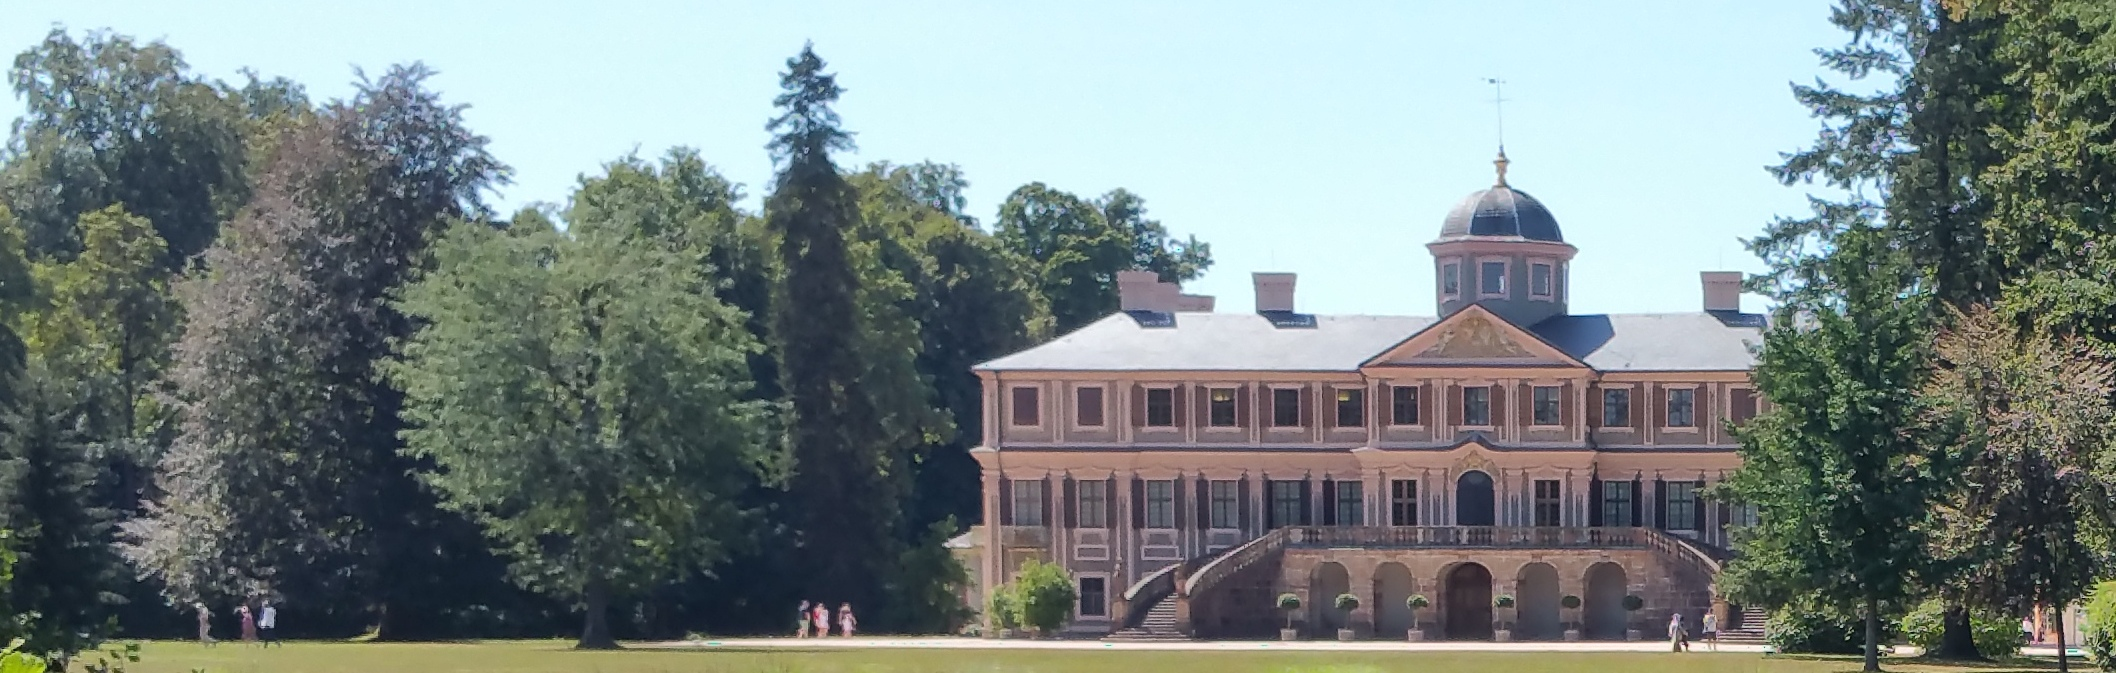
\includegraphics[width=\linewidth]{./images/examples/img-example-01.jpg}%
  \caption[Einbindung eines Bildes]{Beispiel für die Einbindung eines Binärbildes}%
  \label{fig:my-binary-image}%
\end{figure}

Mit Hilfe von Paket \pkg{subfig} \cite{Cochran2005} können Bilder auch in
\index{Abbildung|see{Bild}}\index{Bild!Unterabbildung}Unterabbildungen gesetzt
und sowohl als ganzes (vgl. \cref{fig:subfloat-example}) als auch einzeln (vgl.
\cref{fig:subfloat-example-01,fig:subfloat-example-02,fig:subfloat-example-03,fig:subfloat-example-04})
referenziert werden.

\begin{figure}[H]%
	\centering%
	\subfloat[La Savoureuse, Lepuix, Frankreich (\copyright\ Thomas Bresson)]{%
		\label{fig:subfloat-example-01}%
		\includegraphics[width=0.49\linewidth]{./images/examples/subfloat-example-01.jpg}%
	}%
	\hfill%
	\subfloat[Bangkok, Thailand (\copyright\ Prachanart Viriyaraks)]{%
		\label{fig:subfloat-example-02}%
		\includegraphics[width=0.49\linewidth]{./images/examples/subfloat-example-02.jpg}%
	}%
	\\%
	\subfloat[Wahkeena Falls, Lincoln Park, USA (\copyright\ srslyguys)]{%
		\label{fig:subfloat-example-03}%
		\includegraphics[width=0.49\linewidth]{./images/examples/subfloat-example-03.jpg}%
	}%
	\hfill%
	\subfloat[Nacionalni park Plitvička jezer, Kroatien (\copyright\ Roman Bonnefoy)]{%
		\label{fig:subfloat-example-04}%
		\includegraphics[width=0.49\linewidth]{./images/examples/subfloat-example-04.jpg}%
	}%
	\caption[Bild mit Unterabbildungen]{Wasserfälle der Welt als Beispiel für Unterabbildungen}%
	\label{fig:subfloat-example}%
\end{figure}

Der Beispielcode dafür ist in \cref{lst:subfigures} dargestellt.

\begin{lstlisting}[caption={Unterabbildungen in LaTeX},label={lst:subfigures}]
\begin{figure}[H]%
	\centering%
	\subfloat[Unterbezeichnung 1)]{%
		\label{fig:UnterAbb1}%
		\includegraphics[width=0.49\linewidth]{Bildpfad/Bild1}%
	}%
	\hfill%
	\subfloat[Unterbezeichnung 2]{%
		\label{fig:UnterAbb2}%
		\includegraphics[width=0.49\linewidth]{Bildpfad/Bild2}%
	}%
	\\%
	\subfloat[Unterbezeichnung 3)]{%
		\label{fig:UnterAbb3}%
		\includegraphics[width=0.49\linewidth]{Bildpfad/Bild3}%
	}%
	\hfill%
	\subfloat[Unterbezeichnung 4]{%
		\label{UnterAbb4}%
		\includegraphics[width=0.49\linewidth]{Bildpfad/Bild4}%
	}%
\caption[Kurzversion]{Langversion der Bildunterschrift}%
\label{fig:MeinGanzesBild}%
\end{figure}
\end{lstlisting}


%%%%%%%%%%%%%%%%%%%%%%%%%%%%%%%%%%%%%%%%%%%%%%%%%%%%%%%%%%%%
\subsection[TikZ-Grafiken]{\index{TikZ}\index{Bild!TikZ}\gls{gls:tikz}-Grafiken}%
\label{sec:TikZ}
%%%%%%%%%%%%%%%%%%%%%%%%%%%%%%%%%%%%%%%%%%%%%%%%%%%%%%%%%%%%
%
\Gls{gls:tikz} eignet sich hervorragend, um wissenschaftliche Zeichnungen,
Vektorgrafiken und \index{Diagramm}Diagramme direkt mithilfe von LaTeX
zu setzen, sodass die Schrift direkt zum restlichen Dokument passt.
Zu dem \pkg{tikz}-\gls{gls:pkg} und dem darauf aufsetzenden \pkg{PGFplots}-\gls{gls:pkg} gibt
es hervorragende Dokumentationen \parencites{Tantau2013}{Feuersaenger2014}.
Mit \gls{gls:tikz} und \gls{gls:pgfplots} lassen sich viele gute Sachen machen.


Der Code für die Einbindung einer \gls{gls:tikz}-Grafik steht in \cref{lst:tikz-figure}.
\begin{lstlisting}[caption={Einbindung einer TikZ-Zeichnung in LaTeX},label={lst:tikz-figure}]
\begin{figure}[H]%
  \centering%
  \tikzsetnextfilename{TikZ-Bild}%
  \resizebox{\textwidth}{!}{%   <--- optionale Skalierung
    \input{./figures-src/TikZ-Bild.tex}%
  }%                            <--- optionale Skalierung
  \caption[Kurzversion für das Abbildungsverzeichnis]{%
           Eine tolle sehr lange Abbildungsunterschrift}%
  \label{fig:my-tikz-figure}%
\end{figure}
\end{lstlisting}

Eine Skalierung auf die volle Seitenbreite oder ein vielfaches davon im Falle von Unterabbildungen kann bei Bedarf mit Hilfe der Anweisung
\lstinline|\resizebox{\textwidth}{!}{...}|
durchgeführt werden.

Das Kommando \lstinline|\tikzsetnextfilename{...}| ist nicht unbedingt notwendig,
 aber sehr zu empfehlen, da dies als Name für das temporäre Kompilat im Ordner
\printfilepathquoted{./figures-compiled/} genommen wird.
Dieser sollte gleich dem Namen der Quelldatei (ohne Endung) gewählt werden.
Ansonsten nimmt \texttt{pdflatex} eine hochlaufende Nummer als Dateiname,
was die Fehlersuche sehr erschwert.

Nachfolgend finden sich einige Beispiele für TikZ-Zeichnungen, nämlich
eine Übersicht über die KIT-Corporate-Identity-Farben (\cref{fig:kit-colors}),
ein kommutatives Diagramm (\cref{fig:kpca}),
ein Netzwerkkommunikationsgraph (\cref{fig:net-comm}),
einfache \index{Diagramm!Punkt-}Punktdiagramme (\cref{fig:ica})
und etwas aufwendigere Diagramme mit mehreren
\index{Achsensystem|see{Diagramm}}Achsensystemen (\cref{fig:pca}).

Vorzugsweise sollten für die Grafiken die KIT-Corporate-Identity-Farben verwendet werden,
die sowohl eine RGB"=Definition für die Darstellung online,
als auch eine CMYK"=Definition für den Offset-Druck haben.%
\footnote{Bei Erstellung der Manuskriptversionen
für die Online-Veröffentlichung bzw. für den Offset-Druck
ist auf die korrekte Einstellung der Option \printkeyword{useCMYKcolors}
in der Datei \printfilepathquoted{preambel/AlleSchalter.tex} zu achten
(\printkeyword{false} für die Online-Veröffentlichung und \printkeyword{true} für den Druck!}

\begin{figure}[H]%
	\centering%
  \tikzsetnextfilename{kit-colors}%
	%\resizebox{\textwidth}{!}{%
		\begin{tikzpicture}[
box/.append style={rectangle,inner sep=0pt,outer sep=0pt,minimum size=1.5em,draw=none,fill=#1},
label/.style={font={\ttfamily\footnotesize},anchor=east,inner sep=2pt},
caption/.style={font={\ttfamily\footnotesize},rotate=90,anchor=west,inner sep=0pt},
inner sep=0pt
]
\matrix[row sep=.2em,column sep=.2em] {
  &
\node[caption] {\textbackslash{}KITgreen...};    &
\node[caption] {\textbackslash{}KITblue...};     &
\node[caption] {\textbackslash{}KITblack...};    &
\node[caption] {\textbackslash{}KITpalegreen...};&
\node[caption] {\textbackslash{}KITyellow...};   &
\node[caption] {\textbackslash{}KITorange...};   &
\node[caption] {\textbackslash{}KITbrown...};    &
\node[caption] {\textbackslash{}KITred...};      &
\node[caption] {\textbackslash{}KITlilac...};    &
\node[caption] {\textbackslash{}KITcyanblue...};\\
\node[label] {};               &
\node[box=KITgreen      ] {};  &
\node[box=KITblue       ] {};  &
\node[box=KITblack      ] {};  &
\node[box=KITpalegreen  ] {};  &
\node[box=KITyellow     ] {};  &
\node[box=KITorange     ] {};  &
\node[box=KITbrown      ] {};  &
\node[box=KITred        ] {};  &
\node[box=KITlilac      ] {};  &
\node[box=KITcyanblue   ] {};  \\
\node[label] {...70};      &
\node[box=KITgreen70    ] {};  &
\node[box=KITblue70     ] {};  &
\node[box=KITblack70    ] {};  &
\node[box=KITpalegreen70] {};  &
\node[box=KITyellow70   ] {};  &
\node[box=KITorange70   ] {};  &
\node[box=KITbrown70    ] {};  &
\node[box=KITred70      ] {};  &
\node[box=KITlilac70    ] {};  &
\node[box=KITcyanblue70 ] {};  \\
\node[label] {...50};      &
\node[box=KITgreen50    ] {};  &
\node[box=KITblue50     ] {};  &
\node[box=KITblack50    ] {};  &
\node[box=KITpalegreen50] {};  &
\node[box=KITyellow50   ] {};  &
\node[box=KITorange50   ] {};  &
\node[box=KITbrown50    ] {};  &
\node[box=KITred50      ] {};  &
\node[box=KITlilac50    ] {};  &
\node[box=KITcyanblue50 ] {};  \\
\node[label] {...30};      &
\node[box=KITgreen30    ] {};  &
\node[box=KITblue30     ] {};  &
\node[box=KITblack30    ] {};  &
\node[box=KITpalegreen30] {};  &
\node[box=KITyellow30   ] {};  &
\node[box=KITorange30   ] {};  &
\node[box=KITbrown30    ] {};  &
\node[box=KITred30      ] {};  &
\node[box=KITlilac30    ] {};  &
\node[box=KITcyanblue30 ] {};  \\
\node[label] {...15};      &
\node[box=KITgreen15    ] {};  &
\node[box=KITblue15     ] {};  &
\node[box=KITblack15    ] {};  &
\node[box=KITpalegreen15] {};  &
\node[box=KITyellow15   ] {};  &
\node[box=KITorange15   ] {};  &
\node[box=KITbrown15    ] {};  &
\node[box=KITred15      ] {};  &
\node[box=KITlilac15    ] {};  &
\node[box=KITcyanblue15 ] {};  \\
};

\end{tikzpicture}%
	%}%
	\caption{KIT-Corporate-Identity-Farben}%
  \label{fig:kit-colors}%
\end{figure}

\begin{figure}[H]%
	\centering%
  \tikzsetnextfilename{kpca}%
	%\resizebox{\textwidth}{!}{%
		\begin{tikzpicture}
\node (M) at (0,0) {$M$};
\node (F) [right=5em of M] {$F$};
\node (N) [right=5em of F] {$M'$};

\draw[-latex] (M)--(F) node[above,midway,font=\scriptsize] {$\varphi$};
\draw[-latex] (F)--(N) node[above,midway,font=\scriptsize] {PCA};
\draw[-latex,dotted] (M) to[bend left] node[inner sep=0pt,above=5pt,midway,font=\scriptsize] {kernelized PCA} (N);

\node[below=2ex of M,font=\scriptsize] {$\dim(M) = d$};
\node[below=2ex of F,font=\scriptsize] {$\dim(F) \gg d$};
\node[below=2ex of N,font=\scriptsize] {$\dim(M') = d' < d$};
\end{tikzpicture}%
	%}%
	\caption{Kommutative Diagramm mit TikZ}%
  \label{fig:kpca}%
\end{figure}

\begin{figure}[H]%
	\centering
  \tikzsetnextfilename{net-comm}%
	\resizebox{\textwidth}{!}{%
		\begin{tikzpicture}[
every node/.append style={font={\sffamily},inner sep=2pt},
caption/.append style={font={\sffamily\bfseries}, inner sep=0pt},
comm/.style={-latex,semithick,inner sep=2pt},
msg/.style={midway,sloped,above,font={\sffamily\small},inner sep=2pt},
inner sep=0pt
]
\matrix[row sep=3ex,column sep=25mm] {%
\node[caption] {Partner 1};  & \node[caption] {Partner 2}; & \node[caption] {Partner 3};\\
\node (A1) {Aktion 1}; & & \\
& \node (A2) {Aktion 2}; & \\
\node (A3) {Aktion 3}; & & \\
& & \node (A4) {Aktion 4};\\
& \node (A5) {Aktion 5}; & \\
\node (A6) {Aktion 6}; & & \\
};

\draw[comm] (A1)--(A2) node[msg] {Nachricht 1};
\draw[comm] (A2)--(A3) node[msg] {Nachricht 2};
\draw[comm] (A3)--(A4) node[msg] {Nachricht 3};
\draw[comm] (A4)--(A5) node[msg] {Nachricht 4};
\draw[comm] (A5)--(A6) node[msg] {Nachricht 5};

\end{tikzpicture}%
	}%
	\caption{Netzwerkkommunikationsgraph mit TikZ}%
  \label{fig:net-comm}%
\end{figure}

\begin{figure}[H]%
	\centering%
	\subfloat[Ursprünglicher Merkmalsraum]{%
		\label{fig:ica-1}%
		\tikzsetnextfilename{ica-1}%
		\resizebox{0.45\textwidth}{!}{%
			\input{./figures-src/ica-1.tex}
		}%
	}%
	\hfill%
	\subfloat[Transienter Merkmalsraum (Nach Whitening, z.\,B. durch \gls{ac:PCA} inkl. Normalisierung)]{%
		\label{fig:ica-2}%
		\tikzsetnextfilename{ica-2}%
		\resizebox{0.45\textwidth}{!}{%
			\input{./figures-src/ica-2.tex}%
		}%
	}%
	\hfill%
	\subfloat[Transformierter Merkmalsraum]{%
		\label{fig:ica-3}%
		\tikzsetnextfilename{ica-3}%
		\resizebox{0.45\textwidth}{!}{%
			\input{./figures-src/ica-3.tex}%
		}%
}%
\caption{Diagramme mit TikZ direkt in LaTeX (hier: Die Schritte der \enquote{Independent component analysis})}%
\label{fig:ica}%
\end{figure}

\begin{figure}[H]
	\centering%
	\subfloat[Ungünstige Projektion]{%
		\label{fig:pca-1}%
		\tikzsetnextfilename{pca-1}%
		\resizebox{0.48\textwidth}{!}{%
			\input{./figures-src/pca-1.tex}%
		}%
	}\hfill%
	\subfloat[Zielführende Projektion]{%
		\label{fig:pca-2}%
		\tikzsetnextfilename{pca-2}%
		\resizebox{0.48\textwidth}{!}{%
			\input{./figures-src/pca-2.tex}%
		}%
	}%
	\caption{Aufwändiges Diagramm mit TikZ (hier: Probleme der \enquote{Principal component analysis})}%
	\label{fig:pca}%
\end{figure}
%%%%%%%%%%%%%%%%%%%%%%%%%%%%%%%%%%%%%%%%%%%%%%%%%%%%%%%%%%%%
\section{Tabellen}%
\label{sec:Tabellen}
%%%%%%%%%%%%%%%%%%%%%%%%%%%%%%%%%%%%%%%%%%%%%%%%%%%%%%%%%%%%
Für eine ausführliche Erläuterung auch über gute und schlechte Tabellen
und deren Gestaltung empfiehlt sich die Lektüre des entsprechenden Artikels im \LaTeX{}"=Kompendium auf Wikibooks%
\footnote{\url{https://de.wikibooks.org/wiki/LaTeX-Kompendium:_Tabellen}}
sowie die Dokumentation des \pkg{booktabs}-Pakets \cite{Fear2005}.
\Ua stellt dieses Paket die Befehle
\begin{itemize*}
	\item \lstinline|\toprule|
	\item \lstinline|\midrule|
	\item \lstinline|\bottomrule|
\end{itemize*}
zur Verfügung.

Der Code für eine einfache Tabelle ist im \cref{lst:tabellenbeispiel} angeführt.

\begin{latex}[caption={Einfache Tabelle in \LaTeX},label={lst:tabellenbeispiel}]
\begin{table}%
	\centering%
	\begin{tabularx}{\columnwidth}{l l X}%
		\toprule%
		Datei       &  Bedeutung    &  Benutzerinteraktion \\%
		\midrule%
		Diss.tex  &  Hauptdatei   &  nein     \\%
		images/   &  Bilder       &  ja       \\%
		content/  &  Kapitel      &  ja       \\%
		\bottomrule%
	\end{tabularx}%
	\caption{Dateien der Vorlage}%
	\label{tab:tabellenbeispiel}%
\end{table}
\end{latex}

Das Ergebnis sieht man in \cref{tab:tabellenbeispiel}.

\begin{table}%
	\centering%
	\begin{tabular}{l l l}%
		\toprule%
		Datei       &  Bedeutung    &  Benutzerinteraktion \\%
		\midrule%
		Diss.tex  &  Hauptdatei   &  nein     \\%
		images/   &  Bilder       &  ja       \\%
		content/  &  Kapitel      &  ja       \\%
		\bottomrule%
	\end{tabular}%
	\caption{Dateien der Vorlage}%
	\label{tab:tabellenbeispiel}%
\end{table}

Etwas komplizierter wird es, wenn man eine Tabelle mit alternierender Farbe einfügen möchte (\cref{tab:AlternierendeZeilenfarben}).

\begin{table}%
\caption{Tabelle mit alternierender Zeilenfarbe}%
\label{tab:AlternierendeZeilenfarben}%
	\tablestyle%
	\tablealtcolored%
	\begin{tabular}{*{2}{v{0.45\textwidth}}}%
		\toprule%
		\tableheadcolor%
		\tableheadformat Tabellenkopf &	\tableheadformat Tabellenkopf
		\tabularnewline%
		\midrule%
		%% Zwischenkopf ---------------------------------------------
		\multicolumn{2}{>{\columncolor{tablesubheadcolor}}l}{\bfseries\color{KITblue} Zwischenkopf}%
		\tabularnewline%
		%%-----------------------------------------------------------
		Inhalt  & Inhalt \tabularnewline
		Inhalt  & Inhalt \tabularnewline
		Inhalt  & Inhalt \tabularnewline
		%% Zwischenkopf ---------------------------------------------
		\multicolumn{2}{>{\columncolor{tablesubheadcolor}}l}{\bfseries\color{KITgreen} Zwischenkopf}%
		\tabularnewline
		%%-----------------------------------------------------------
		Inhalt  & Inhalt \tabularnewline
		Inhalt  & Inhalt \tabularnewline
		\bottomrule%
	\end{tabular}%
\end{table}

%% ------------------------------------------------------------
Lange Tabellen, die umbrochen werden sollen, können mit
\lstinline|\LTXtable{\textwidth}{Datei}|
eingebunden werden, wobei die Tabelle in eine Datei ausgelagert werden muss.
Ein Beispiel dafür sieht man in \cref{tab:MehrseitigeTabelle}.

\IfDefined{LTXtable}{%
	%--Einstellungen für Tabellen ----------
	\colorlet{tablerowcolor}{gray!10.0}%
	\renewcommand\tableheadcolor{\rowcolor{tableheadcolor}}%
	\renewcommand\tablehead{%
			\tableheadfontsize%
			\sffamily\bfseries%
			\slshape%
			\color{black}%
	}%
	%---------------------------------------
	{
		\tablestyle%
		%\tablealtcolored
		\rowcolors{1}{tablerowcolor}{white!100}%
		 \LTXtable{\textwidth}{tables/LongTableExample.tex}%
	}%
} % End If 
%
%
%
Sollten eine Tabelle so breit sein, dass sie nicht mehr horizontal auf
eine Seite passt, so ist es natürlich möglich, diese mithilfe des Pakets
\printkeyword{rotfloat} \parencite{Sommerfeldt2004} in eine
\printkeyword{sidewaystable} statt in eine \printkeyword{table}-Umgebung zu setzen.
Also so:
\begin{latex}[caption={Gedrehte Tabelle},label={lst:rotated-table}]
\begin{sidewaystable}
  \centering%
  \begin{tabular}{...}%
    ...
  \end{tabular}%
  \caption{Bezeichnung}%
  \label{Referenzmarke}%
\end{sidewaystable}%
\end{latex}

Das Ergebnis sieht man in \cref{tab:ex-sideways}.

%% Um 90° gedrehte Tabelle
%
\begin{sidewaystable}[p]
\tablestylecommon%
\scriptsize% hier ausnahmsweise kleine Schriftgröße
\raggedleft% Rechtsbündig, damit die Tabelle oben ausgerichtet wird (Forderung KSP)
\begin{tabular}{l M M M M M}%
\toprule%
\addlinespace[0pt]%
 & \multicolumn{5}{c}{\bfseries Level} \tabularnewline
 & \multicolumn{2}{c}{\bfseries Qualitative} & \multicolumn{3}{c}{\bfseries Quantitative} \tabularnewline
 & \bfseries\centering Nominal & \bfseries\centering Ordinal & \bfseries\centering Interval & \bfseries\centering Ratio & \bfseries\centering Absolute \tabularnewline \addlinespace[0pt]\midrule\addlinespace[0pt]
Empirical relation &
\begin{tabitemize}\item[$\sim$] Equivalence\end{tabitemize} &
\begin{tabitemize}\item[$\sim$] Equivalence\item[$\prec$] Ordering\end{tabitemize} &
\begin{tabitemize}\item[$\sim$] Equivalence\item[$\prec$] Ordering\end{tabitemize} &
\begin{tabitemize}\item[$\sim$] Equivalence\item[$\prec$] Ordering\strut\end{tabitemize} &
\begin{tabitemize}\item[$\sim$] Equivalence\item[$\prec$] Ordering\strut\end{tabitemize} \tabularnewline \midrule
Empirical operation &
 &
 &
\begin{tabitemize}\item[$\oplus$] Addition\end{tabitemize} &
\begin{tabitemize}\item[$\oplus$] Addition\item[$\otimes$] Multiplication\strut\end{tabitemize} &
\begin{tabitemize}\item[$\oplus$] Addition\item[$\otimes$] Multiplication\strut\end{tabitemize} \tabularnewline \midrule
Feasable transformation &
$m' = f( m )$ for $f$ bij.\strut &
$m' = f( m )$ for $f$ mon.\strut &
$m' = am + b$ for $a>0$\strut &
$m' = am$ for $a>0$\strut &
$m' = m$\strut \tabularnewline \midrule
Examples of features &
\begin{tabitemize}\item Telephone numbers\item Postal codes\item Gender\strut\end{tabitemize} &
\begin{tabitemize}\item Grades\item Degree of hardness\item Wind intensity\strut\end{tabitemize} &
\begin{tabitemize}\item Temperatur in F\textdegree\item Calendric time\item Geographic altitude\strut\end{tabitemize} &
\begin{tabitemize}\item Temperatur in K\item Mass\item Length\item Electric current\strut\end{tabitemize} &
\begin{tabitemize}\item Quantum numbers\item Error number\strut\end{tabitemize} \tabularnewline \midrule
Range of features &
\begin{tabitemize}\item Numbers\item Names\item Symbols\strut\end{tabitemize} &
Natural numbers &
Real numbers &
Real, positive numbers &
Natural numbers \tabularnewline \midrule
Expressiveness & low & \dots & \dots & \dots & high\strut \tabularnewline \addlinespace[0pt]
\bottomrule%
\end{tabular}%
\caption{Beispiel für eine breite, gedrehte Tabelle (hier: Taxonomie der Maßskalen)}%
\label{tab:ex-sideways}%
\end{sidewaystable}
%%%%%%%%%%%%%%%%%%%%%%%%%%%%%%%%%%%%%%%%%%%%%%%%%%%%%%%%%%%%
\section{Mathematische Sätze, Lemmas, Definitionen etc.}%
\label{sec:Theoreme}
%%%%%%%%%%%%%%%%%%%%%%%%%%%%%%%%%%%%%%%%%%%%%%%%%%%%%%%%%%%%
%
Für eine mathematische Ausarbeitung gibt es LaTeX-\glspl{gls:umgebung}, um
\index{Satz|see{Theorem}}\index{Theorem}Sätze (Theoreme), \index{Lemma|see{Theorem}}Lemma,
\index{Beispiel|see{Theorem}}Beispiele \etc im üblichen Stil von
Mathematik-Büchern zu setzen und zu referenzieren. Vordefiniert sind die
\glspl{gls:umgebung}
\begin{itemize*}
  \item \texttt{theorem} für Sätze
  \item \texttt{definition} für Definitionen
  \item \texttt{lemma} für Lemma
  \item \texttt{corollary} für Korollare
  \item \texttt{proposition} für Propositionen
\end{itemize*}
Die übliche Verwendung ist
\begin{latex}[caption={Beispiel für Theorem-Umgebungen},label={lst:ntheorem}]
\begin{theorem}[Optionaler Name]\label{thm:my-theorem}
...
\end{theorem}
\end{latex}
Weitere Informationen findet man in der Dokumentation zum \texttt{ntheorem}-Paket
\parencite{May2011}. Das Ganze sieht dann beispielsweise wie folgt aus.

\begin{theorem}[Theorem von Arthur Dent]
\label{thm:arthur-dent} Die Antwort auf die Frage nach dem Leben, dem Universum und den ganzen Rest ist 42.
\end{theorem}

\begin{definition}
\LaTeX{} ist eine von Leslie Lamport 1980 entwickelter Satz von Makros zur Erweiterung von \TeX.
\end{definition}

\begin{proposition}[Zweifelhafte Folgerung]
LaTeX ist schön. Beweis folgt unmittelbar aus \cref{thm:arthur-dent}.
\end{proposition}

%%%%%%%%%%%%%%%%%%%%%%%%%%%%%%%%%%%%%%%%%%%%%%%%%%%%%%%%%%%%
\section{Quellcode-Listings}%
\index{Listing!Gestaltungsstil}%
\label{sec:Listings}
%%%%%%%%%%%%%%%%%%%%%%%%%%%%%%%%%%%%%%%%%%%%%%%%%%%%%%%%%%%%
%
Zum Einbinden und Formatieren von \index{Code|see{Listing}}Quellcode"=Beispielen
-- sog. \index{Listing}Listings -- wird das Paket \pkg{listings}
\parencite{Hoffmann2014} verwendet.
Das Hervorheben von \index{Schlusselwort@Schlüsselwort}Schlüsselwörtern
wird von LaTeX automatisch erledigt,
wenn die korrekte Sprache des Listings angegeben ist.
Dies geschieht mit Hilfe der Option \printkeyword{language}
oder durch die Angabe eines entsprechend definierten Gestaltungsstils.

Im Befehl \lstinline|\lstset{...}|,
welcher in der Datei \printfilepath{preambel/preambel.tex} zu finden ist,
kann man einen globalen Stil für alle Listings vorgeben
(welcher jedoch bei Bedarf im Einzelfall überrufen werden kann).
Aktuell ist der etwas weiter oben im Code mit dem Befehl
\lstinline|\lstdefinestyle{...}| vordefinierte Stil
\printkeyword{latex} als Standardgestaltungsstil ausgewählt.

Neben \printkeyword{latex} sind in der Datei \printfilepath{preambel/preambel.tex}
auch noch \printkeyword{java} und \printkeyword{C++} als Gestaltungsstile vordefiniert.
Bei Bedarf lassen sich dort weitere Stile definieren und auswählen.

Zur Vereinfachung der Einbindung wurden zusätzlich Umgebungen
\printkeyword{latex}, \printkeyword{java} und \printkeyword{C++}
vordefiniert, die im Code mit \lstinline|\begin{<name>}...\end{<name>}|
direkt verwendet werden können (s. \cref{lst:java-listing}).
%
\begin{latex}[caption={Beispiel eines Listings in Java},label={lst:java-listing}]
\begin{java}[caption={Ein Hello-World Beispiel in Java},%
             label={lst:hello-world}]
public class HelloWorld {
  public static void main( String[] args ) {
    System.out.println( "HelloWorld" );
  }
}
\end{java}
\end{latex}
%
Dieses Listing bewirkt das folgende Ergebnis:
%
\begin{java}[caption={Ein Hello-World Beispiel in Java},label={lst:hello-world}]
public class HelloWorld {
  public static void main( String[] args ) {
    System.out.println( "HelloWorld" );
  }
}
\end{java}

Man beachte, dass anders als bei Abbildungen und Tabellen
die Bezeichnung (\texttt{caption}) und die Referenzmarke (\texttt{label})
nicht als gesonderte Befehle, sondern als optionale Argumente übergeben werden.
Dies liegt daran, dass ein Listing in der Regel keine Fließumgebung ist,
sondern an der Stelle im Text erscheint, an der sie im Code auch steht.
Ferner folgt ein Listing den ganz normalen Seitenumbruchsregeln.
Das heißt, ein überlanger Code wird einfach umgebrochen. 
Um ein Listing zu einem Fließobjekt zu machen, muss das optionale Argument
\texttt{float=<tbp>} angegeben werden.
Die \index{Platzierung}Plazierungsangabe \enquote{\texttt{h}} für \enquote{hier}
ist nicht erlaubt. Denn dies ist das Standardverhalten ohne \texttt{float}.
%%%%%%%%%%%%%%%%%%%%%%%%%%%%%%%%%%%%%%%%%%%%%%%%%%%%%%%%%%%%
\section{Mathematik}%
\label{sec:Mathe}
%%%%%%%%%%%%%%%%%%%%%%%%%%%%%%%%%%%%%%%%%%%%%%%%%%%%%%%%%%%%
%
Grundsätzlich gilt, was in \parencites{ams1999a}{ams1999b} steht. In der Datei
\printfilepath{preambel/Math.tex} sind eine Menge Kurzkommandos definiert,
um eine einheitliche Typografie von
\index{Skalare}Skalaren, \index{Vektoren}Vektoren, \index{Matrizen}Matrizen,
\index{Zufallsvariablen}Zufallsvariablen etc. zur vereinfachen.
In diese Dateien einfach mal reinschauen, welche Kurzkommandos es gibt.

Grundsätzlich empfiehlt es sich, eigene Mathe-Makros zu definieren und durchgehend zu verwenden.
Damit kann man bei Bedarf die Formatierung der Variablen an einer einzigen Stelle anpassen,
ohne den gesamten Code des Arbeit durchgehen zu müssen.

Die Einbettung der Formeln geschieht mit der \printkeyword{equation}"=Umgebung.
Da die Formeln normalerweise keine eigenständigen Absätze darstellen,
sollen zwischen dem Fließtext und der Formeldefinition keine leeren Zeilen stehen,
da \LaTeX{} diese als Absätze behandelt und unnötigerweise zusätzliche vertikale Abstände hinzufügt.

Auch sollte man darauf achten, dass zwischen einer Zahl und der physikalischen Einheit ein umbruchgeschütztes Leerzeichen verwendet wird.
Allerdings sollte statt dem üblichen (dehnbaren) umbruchgeschützen Wortzwischenraum, 
welches mit einer Tilde erzeugt wird, ein schmälerer Abstand verwendet werden.
Dieser wird mit \verb+\,+  erzeugt und beträgt standardmäßig 0,1667\,em. Dies geht so:
%
\begin{inlinelatex}
Der eingefügte Abstand beträgt 0,1667\,em.
\end{inlinelatex}

Auf zwei besondere Kommandos wird näher eingegangen,
weil dies in \LaTeX{} häufig falsch gemacht wird.
\begin{itemize}
  \item Für die Matrixtransponierte gibt es das Kommando \verb#\Tr#, also
	\verb#$A^{\Tr}$# liefert $A^{\Tr}$	
	\item Bei \index{Integral}Integralen muss das \enquote{Differential-d} gemäß
	ISO in aufrechter Schrift als Operator gesetzt sein mit einem kleinen Abstand
	zum Integranden. Hierfür gibt es das spezielle Kommando \verb#\diff#.
	\Dhe, die Schreibweise \verb#\int^1_0 x^2 d x = \frac{1}{3}# (\cref{eq:Diff-wrong}) ist falsch,
	während \verb#\int^1_0 x^2 \diff x = \frac{1}{3}# (\cref{eq:Diff-correct}) das Richtige liefert:
\end{itemize}
\begin{equation}
	\int^1_0 x^2 d x = \frac{1}{3} \qquad \text{(falsche Typografie!)}
	\label{eq:Diff-wrong}
\end{equation}
\begin{equation}
	\int^1_0 x^2 \diff x = \frac{1}{3} \qquad \text{(richtige Typografie!)}
	\label{eq:Diff-correct}
\end{equation}


\input{content/0X-ExampleContents/Querverweise.tex}
%%%%%%%%%%%%%%%%%%%%%%%%%%%%%%%%%%%%%%%%%%%%%%%%%%%%%%%%%%%%
\section{Literaturverzeichnisse}%
\label{sec:Literaturverzeichnisse}%
\index{Bibliografie}\index{Literaturverzeichnis}
%%%%%%%%%%%%%%%%%%%%%%%%%%%%%%%%%%%%%%%%%%%%%%%%%%%%%%%%%%%%
%
Defaultmäßig befinden sich alle Literaturangaben in der Datei
\printfilepathquoted{bib/Diss.bib}.
Falls ein davon abweichender Pfad oder weitere Literaturdatenbanken
verwendet werden sollen, können entsprechende Pfade in der Datei
\printfilepathquoted{preambel/AllePfade.tex} mit
\lstinline|\addbibresource{...}|
festgelegt werden.
Bitte beachten, dass bei den Literaturdatenbanken kein \gls{gls:bibtex}-,
sondern \gls{gls:biblatex}-Format verwendet werden soll,
also Umlaute direkt eingegeben werden können.

Die Vorlage ermöglicht es, neben dem Haupt"=Literaturverzeichnis
jeweils separat durchnummerierte Listen der eigenen Publikationen und Patente
sowie der betreuten studentischen Arbeiten zu erstellen.
Standardmäßig werden alle Literaturangaben aus der Hauptliteraturdatenbank
\printfilepathquoted{bib/Diss.bib} extrahiert.
Durch Änderung der Definitionen der Pfade
\printkeyword{bibpathOwnPatents},
\printkeyword{bibpathOwnPublications} und
\printkeyword{bibpathStudentTheses}
in der Datei
\printfilepathquoted{preambel/AllePfade.tex}
können jedoch für die einzelnen Auflistungen 
jeweils eigene, speziell dafür angelegte Datenbanken verwendet werden.

Die Einbindung der Literaturverzeichnisse in das Manuskript erfolgt in der Datei
\printfilepathquoted{content/Inhalt-BackMatter.tex}.
Die Zusatz"=Literaturverzeichnisse werden separat erstellt und sind vom Haupt"=Literaturverzeichnis unabhängig.
Dazu werden in den entsprechenden Abschnitten der Datei,
welche jeweils mit Hilfe der \printkeyword{refsection}"=Umgebung abgegrenzt sind,
die kompletten Inhalte der jeweiligen Literaturdatenbank unsichtbar referenziert.
Dies geschieht mit dem \lstinline|\nocite{*}|"=Befehl.
Alternativ dazu können die einzelnen Werke mit
\lstinline|\nocite{Quelle1,Quelle2,...,QuelleN}|
explizit referenziert werden.

Sofern man eine einzige Datenbank für sämtliche Literaturverzeichnisse verwendet
und die unsichtbare Referenzierung jeweils mit dem \lstinline|\nocite{*}|"=Befehl erfolgt,
müssen die relevanten Referenzen für das jeweilige Zusatz"=Literaturverzeichnis
gefiltert werden.
Die Filterung der eigenen Publikationen, Patente und betreuten Arbeiten
für die einzelnen Verzeichnisse geschieht jeweils mit der Angabe
\lstinline|keyword=ownpubl|,
\lstinline|keyword=ownpatent|
oder
\lstinline|keyword=supervised|
in der Optionenliste des jeweiligen
\lstinline|printbibliography|"=Befehls.
Dazu müssen die Literatureinträge in der Literaturdatenbank freilich
entsprechend jeweils mit der Angabe
\lstinline|keywords = {ownpubl}|,
\lstinline|keywords = {ownpatent}|
oder
\lstinline|keywords = {supervised}|
versehen werden.

Bei Verwendung separater Literaturdatenbanken für die einzelnen Zusatzverzeichnisse
oder bei einer expliziten Aufzählung der einzelnen Veröffentlichungen mit dem
\lstinline|\nocite{Quelle1,Quelle2,...,QuelleN}|"=Befehl,
ist eine Filterung der Literaturdatenbank nach einem Keyword nicht notwendig.
Damit könnte die Notwendigkeit von Zusatzangaben in der Literaturdatenbank entfallen.
Allerdings muss dann auch die standardmäßig gesetzte Filter-Option in den jeweiligen
\lstinline|printbibliography|"=Befehlen
in der Datei  \printfilepathquoted{content/Inhalt-BackMatter.tex}
deaktiviert (sprich auskommentiert) werden.

Die Zusatzauflistungen sind von den Zitierungen im Text unabhängig.
Damit ergibt sich für eigene Veröffentlichungen,
die im Text explizit zitiert werden, eine doppelte Listung --
einmal in der Hauptliteraturliste (mit einer alphanumerischen Referenz)
und einmal in der durchnummerierten Liste eigener Publikationen.
Dies ist kein Bug, sondern ein Feature der Vorlage.

Bei der Auflistung eigener Veröffentlichungen und Patente ist 
in der Vorlage jeweils ein kleines Vorwort vorgesehen.
Darin können beispielsweise Zusatzhinweise zur Abgrenzung der Publikationen bzw.
der Patente, die während der Promotionszeit entstanden sind,
oder Hinweise zur Eingruppierung der Veröffentlichungen platziert werden.
Diese einleitenden Texte sind ebenfalls in der Datei
\printfilepathquoted{content/Inhalt-BackMatter.tex}
definiert und können dort editiert werden.

Bei der Erwähnung der einzelnen eigenen Veröffentlichungen und Patente in den Vorworten 
zu den jeweiligen Listen
muss die Einbindung mit Hilfe des Makros
\lstinline|\citefield{...}[labelnumberwidth]{labelnumber}|
statt der üblichen Einbindung mit dem Makro
\lstinline|\cite{...}|
erfolgen, damit die zu den Listen passende (nummerische) Formatierung verwendet wird.

Sind keine Vorworte vor den Listen eigener Veröffentlichungen und Patente erwünscht,
lassen sich diese durch die Auskommentierung der Optionen
\lstinline|prenote=OwnPublPrenote|
\bzw
\lstinline|prenote=OwnPatentPrenote|
in den jeweiligen 
\lstinline|printbibliography|"=Befehlen komplett ausblenden.
%%%%%%%%%%%%%%%%%%%%%%%%%%%%%%%%%%%%%%%%%%%%%%%%%%%%%%%%%%%%
\section{Abkürzungsverzeichnis, Stichwortverzeichnis (Index), Symbolverzeichnis und Glossar}%
\index{Abkürzungsverzeichnis}%
\index{Glossar}%
\index{Symbolverzeichnis}%
\index{Stichwortverzeichnis}%
%\index{Index|see{Stichwortverzeichnis}}
\label{sec:Glossare}
%%%%%%%%%%%%%%%%%%%%%%%%%%%%%%%%%%%%%%%%%%%%%%%%%%%%%%%%%%%%
%
Die Vorlage unterstützt auch ein Abkürzungsverzeichnis, ein Stichwortverzeichnis,
ein Symbolverzeichnis sowie ein allgemeines \index{Glossar}\gls{gls:Glossar},
das Definitionen von \index{Fachbegriff!Definition}Fachtermini oder
\index{Uebersetzung@Übersetzung}Übersetzungen von fremdsprachlichen Begriffen
(d.h. eine Art Lexikons) enthalten kann.


%%%%%%%%%%%%%%%%%%%%%%%%%%%%%%%%%%%%%%%%%%%%%%%%%%%%%%%%%%%%
\subsection*{Abkürzungen und Abkürzungsverzeichnis}%
\index{Abkürzungen}%
\index{Akronyme}%
\label{sec:Akronyme}
%%%%%%%%%%%%%%%%%%%%%%%%%%%%%%%%%%%%%%%%%%%%%%%%%%%%%%%%%%%%
Zur Erzeugung des Abkürzungsverzeichnises und des Glossars wird intern das
\pkg{glossaries}-\gls{gls:pkg} verwendet \cite{talbot2014}.
Zudem wurden einige Makros definiert, welche die Erfassung der Begriffe erleichtern sollen.
%
Um ein Abkürzungsverzeichnis zu erzeugen, muss zuerst eine Liste der Abkürzungen angelegt werden.
Dies geschieht in der Datei \printfilepathquoted{./preambel/Acronyms.tex}.
Hierfür wird das Makro \lstinline|\newacronym| verwendet.
Dieses Makro hat drei obligatorische Argumente, nämlich
\begin{itemize*}
\item die Marke,
\item das Akronym und
\item die Langform.
\end{itemize*}

Als Konvention wird der Marke eines Akronyms \printkeyword{ac:} als Präfix vorangestellt.

\begin{latex}[caption={Definition einer Abkürzung},label={lst:SimpleAcronymEntry}]
\newacronym{ac:MSA}{MSA}{mein schönes Akronym}
\end{latex}

Optional können Pluralformen, sowie Genitiv-, Dativ- und Akkusativ-Formen 
der Abkürzung und des eigentlichen Begriffs angegeben werden,
sofern sie im Quelltext verwendet werden und sich von der Grundform unterscheiden.
Außerdem kann mit dem Schlüsselwort \printkeyword{description}
eine abweichende Version der Langform für die Verwendung im Abkürzungsverzeichnis definiert werden:

\begin{latex}[caption={Definition einer Abkürzung mit Zusatzangaben},label={lst:AdvancedAcronymEntry}]
\newacronym[shortgenitive={MSAs},%
            genitive={meines schönen Akronyms},%
            %shortdative={MSA},% <- entspriht der Hauptform 
            %            % ==> keine Zusatzdefinition nötig!
            dative={meinem schönen Akronym},%
            %shortaccusative={MSA},%
            %accusative={mein schönes Akronym},%
            shortplural={MSAs},
            longplural={meine schönen Akronyme},%
            %shortpluralgenitive={MSAs},%
            pluralgenitive={meiner schönen Akronyme},%
            %shortpluraldative={MSAs},%
            pluraldative={meinen schönen Akronymen},%
            %shortpluralaccusative={MSAs},%
            pluralaccusative={meine schönen Akronyme},%
            description={mein schönes Akronym, % <- optional!
                         ein Beispiel für eine Abkürzung}%
           ]{ac:MSA}{MSA}{mein schönes Akronym}
\end{latex}

Im Text des Dokumentes werden die Einträge durch den Befehl \lstinline|\ac{<Marke>}| verwendet.
Bei der erstmaliger Verwendung wird die Langform gedruckt, gefolgt von der Abkürzung, welche in Klammern gesetzt wird.
Beim zweiten Vorkommen wird nur noch die Abkürzung gedruckt.
Zusätzlich definiert die Vorlage die Befehle
\lstinline|\acgen{...}|, \lstinline|\acdat{...}| und \lstinline|\acacc{...}|, sowie
\lstinline|\acplgen{...}|, \lstinline|\acpldat{...}| und \lstinline|\acplacc{...}|,
die jeweils die Genitiv-, Dativ- und Akkusativ-Form (Singular und Plural) drucken.

Im \gls{gls:pkg} \pkg{glossaries} stellt der Befehl \lstinline|\ac{...}| ein Shortcut für den Befehl \lstinline|\gls{...}| dar.
Mit diesem kann ein allgemeiner Glossar-Eintrag im Text referenziert werden.

Mit den Befehlen
\lstinline|\acrshort{...}|, \lstinline|\acrlong{...}|, \lstinline|\acrfull{...}|
und ihren Abwandlungen sowie den Shortcuts
\lstinline|\acs{...}|, \lstinline|\acl{...}|, \lstinline|\acf{...}|,
kann jeweils nur die Abkürzung, nur die Langform oder beides explizit angefordert werden.
Allerdings wird eine solche Verwendung ggf. nicht als \enquote{erstmalige Verwendung} zählen.

Damit resultiert der folgende Quellcode
\begin{latex}[caption={Verwendung von Abkürzungen},label={lst:AcronymUsage}]
    \Acf{ac:MSA} ist ein Beispiel für die Verwendung
    einer Abkürzung am Anfang des Satzes. Man beachte,
    dass der Aufruf der Marke mit dem Makro
    \lstinline|\acf{...}| bzw. \lstinline|\Acf{...}|
    nicht als die erste Erwähnung im Text zählt.
    Bei der ersten Nennung \acgen{ac:MSA} unter
    Verwendung der Makros \lc{ac}, \lc{acgen} \oae
    erscheint die Langform, gefolgt von der Kurzform.
    Bei der zweiten Nennung \acgen{ac:MSA}
    erscheint nur noch die Kurzform \ac{ac:MSA}.
\end{latex}
%
in der folgenden Ausgabe:
%
\begin{quote}
    \Acf{ac:MSA} ist ein Beispiel für die Verwendung
    einer Abkürzung am Anfang des Satzes. Man beachte,
    dass der Aufruf der Marke mit dem Makro
    \lstinline|\acf{...}| bzw. \lstinline|\Acf{...}|
    nicht als die erste Erwähnung im Text zählt.
    Bei der ersten Nennung \acgen{ac:MSA} unter
    Verwendung der Makros \lc{ac}, \lc{acgen} \oae
    erscheint die Langform, gefolgt von der Kurzform.
    Bei der zweiten Nennung \acgen{ac:MSA}
    erscheint nur noch die Kurzform \ac{ac:MSA}.
\end{quote}


%%%%%%%%%%%%%%%%%%%%%%%%%%%%%%%%%%%%%%%%%%%%%%%%%%%%%%%%%%%%
\subsection*{Glossar}%
\index{Glossar}%
\label{sec:Glossar}
%%%%%%%%%%%%%%%%%%%%%%%%%%%%%%%%%%%%%%%%%%%%%%%%%%%%%%%%%%%%

Neben einem Abkürzungsverzeichnis kann man auch ein
\gls{gls:Glossar} erstellen lassen.
In diesem können Definitionen von \index{Fachbegriff!Definition}Fachtermini oder
\index{Uebersetzung@Übersetzung}Übersetzungen von fremdsprachlichen Begriffen stehen.

Der wesentliche Unterschied zwischen einer Abkürzung und einem allgemeinen Glossar-Eintrag ist,
dass bei Abkürzungen bei erstmaliger Verwendung die Abkürzung gedruckt und die Langform in Klammer dahinter gesetzt wird.
Bei allgemeinen Glossar-Einträgen wird normalerweise nur der Name gesetzt.
Durch eine Option des \pkg{glossaries}-\glsgen{gls:pkg} kann man sicher stellen,
dass alle Glossar-Einträge auf das Glossar am Ende des Manuskripts verlinkt werden.
Standardmäßig ist diese Option jedoch deaktiviert.

Die Glossar-Einträge werden in der Datei  \printfilepathquoted{./preambel/Glossary.tex} definiert.

Die Definition der Glossar-Einträge geschieht mit dem Makro \lc{myglossaryentry},
welches drei obligatorische Argumente hat, nämlich
\begin{itemize*}
\item die Marke,
\item den Begriff und
\item die Erklärung / Definition / Übersetzung.
\end{itemize*}
Als Konvention wird der Marke eines Glossar-Eintrages ein \enquote{gls:} als Präfix vorangestellt.
Optional kann die Plural-, sowie Genitiv-, Dativ- und Akkusativ"=Form des Begriffs angegeben werden,
sofern sie im Quelltext verwendet werden und sich von der Grundform unterscheiden.

Ein Glossar-Eintrag kann beispielsweise folgendermaßen definiert werden:
\begin{latex}[caption={Definition eines Glossar-Eintrages},label={lst:GlossEntry}]
\myglossaryentry[plural={Glossare},%
                 genitive={Glossars}]%
                {gls:Glossare}{Glossar}{alphabetisch sortierte Liste von Begriffen mit Erklärung}
\end{latex}

Normalerweise werden im Glossar nur diejenigen Begriffe angezeigt,
die im Text des Dokumentes erwähnt und entsprechend referenziert worden sind.
Eine Referenzierung der Glossar-Einträge im Text geschieht normalerweise mit dem
\lstinline|\gls{<Marke>}|-Befehl,
welcher den Begriff im Text druckt und für seine Aufnahme ins Glossar sorgt.
Weitere mögliche Befehle sind \lstinline|\Gls{...}| und \lstinline|\GLS{...}|,
die den ersten bzw. alle Buchstaben in Großbuchstaben umwandeln,
\lstinline|\glspl{...}|, \lstinline|\Glspl{...}|, \lstinline|\GLSpl{...}|
für die Pluralform usw.
Zusätzlich definiert die Vorlage die Befehle
\lstinline|\glsgen{...}|, \lstinline|\glsdat{...}| und \lstinline|\glsacc{...}|,
sowie
\lstinline|\glsplgen{...}|, \lstinline|\glspldat{...}| und \lstinline|\glsplacc{...}|,
die jeweils die Genitiv- Dativ- und Akkusativ-Form drucken.

Außerdem gibt es mit dem Befehl \lstinline|\glsadd{...}| die Möglichkeit,
eine Stelle im Text mit einem Glossar-Begriff zu verlinken, ohne diesen explizit zu drucken.
Mit \lstinline|\glsaddall| kann man alle definierte Glossar-Einträge ins Glossar aufnehmen,
ohne sie im Text des Dokumentes referenziert zu haben.

Die Verwendung des oben definierten Eintrages im Text mit dem Befehl
\lstinline|\glsgen{gls:Glossar}| mündet im Text in einer Erwähnung des \glsgen{gls:Glossar}.


%%%%%%%%%%%%%%%%%%%%%%%%%%%%%%%%%%%%%%%%%%%%%%%%%%%%%%%%%%%%
\subsection*{Symbolverzeichnis}%
\index{Symbolverzeichnis}%
\index{Symbole}%
\index{Notation}%
\label{sec:Symbolverz}
%%%%%%%%%%%%%%%%%%%%%%%%%%%%%%%%%%%%%%%%%%%%%%%%%%%%%%%%%%%%
%
Ein Symbolverzeichnis kann auf zwei Arten angelegt werden.
Normalerweise reicht eine manuell erstellte Übersicht über die Notation,
so wie sie in der Datei \printfilepathquoted{./00-Front-Matter/Notation.tex}
mit Hilfe von Befehlen
\lstinline|\myNotationTableEntryMath{<Mathe-Ausdruck>}{<Beschreibung>}|
und
\lstinline|\myNotationTableEntryText{<Text-Ausdruck>}{<Beschreibung>}|
definiert wird.
Diese ist recht einfach und lässt sich bei Bedarf beliebig ergänzen.

Allerdings gibt es auch die Möglichkeit zur automatischen Erzeugung eines
Symbolverzeichnisses mit Hilfe des \pkg{glossaries}-\glsgen{gls:pkg}.
Um dieses automatisch generierte Symbolverzeichnis zu erzeugen,
müssen Symbole in Form von Glossar-Einträgen angelegt und im Text des Dokumentes
zumindest einmal entsprechend mit dem Befehl \lstinline|\gls{<Marke>}| referenziert werden.
Dafür müsste ein Symboleintrag folgendermaßen angelegt werden:
\begin{latex}[caption={Definition eines Symboleintrages},label={lst:SymbEntry}]
\newglossaryentry{symb:pi}{%
                  name={\ensuremath{\pi}},%
                  sort={pi},%
                  type=symbols,%
                  description={Kreiszahl, Verhältnis des Umfangs eines Kreises zu seinem Durchmesser}%
                 }
\end{latex}
Die Referenzierung des Symbols \gls{symb:pi} im Text geschieht dann mit 
\lstinline|\gls{symb:pi}|.

In der Vorlage sind beide Arten von Symbolverzeichnissen vorgesehen.
Sie werden am Anfang des Manuskriptes vor dem Inhaltsverzeichnis eingebunden.
Es passiert in der Datei \printfilepathquoted{./content/Inhalt-FrontMatter.tex}.
Bei Bedarf lässt sich diese Einbindung auch an eine geeignete Stelle in den Backmatter verschieben.

Zum einfachen Ein- bzw. Ausblenden der beiden Symbolverzeichnisse
gibt es in der Datei \printfilepathquoted{preambel/AlleSchalter.tex}
die beiden Schalter
\begin{itemize*}
\item \printkeyword{showNotation} für den manuell erstelle Notationübersicht
\item \printkeyword{showListOfSymbols} für das automatisch erstelltes Symbolverzeichnis.
\end{itemize*}



%%%%%%%%%%%%%%%%%%%%%%%%%%%%%%%%%%%%%%%%%%%%%%%%%%%%%%%%%%%%
\subsection*{Stichwortverzeichnis (Index)}%
\index{Stichwortverzeichnis}%
\index{Index|see{Stichwortverzeichnis}}%
\label{sec:Index}
%%%%%%%%%%%%%%%%%%%%%%%%%%%%%%%%%%%%%%%%%%%%%%%%%%%%%%%%%%%%
%
Ein \index{Stichwortverzeichnis}Stichwortverzeichnis (oder Index)
ist einfach nur eine alphabetisch sortierte Liste von Begriffen mit einer Auflistung der Fundstellen im Dokument.
Diese ist nützlich, wenn sich der Leser zu einem Begriff alle Vorkommnisse anschauen möchte.
Der Index wird erzeugt, indem im Quellcode der Befehl \lstinline+\index{Begriff}+
eingefügt wird. Der Begriff selbst wird dadurch nicht gedruckt und muss daher
noch einmal wiederholt werden, um auch im Text gedruckt zu werden. Dieses Verhalten
ist beabsichtigt, sodass im Index immer nur die Grundform des Wortes verwendet
wird, aber im Text natürlich die richtige Deklination.

%%%%%%%%%%%%%%%%%%%%%%%%%%%%%%%%%%%%%%%%%%%%%%%%%%%%%%%%%%%%
\section{Randnotizen und TODO-Notizen}%
\index{Randnotizen}%
\index{TODO-Notizen}%
\label{sec:Randnotizen}
%%%%%%%%%%%%%%%%%%%%%%%%%%%%%%%%%%%%%%%%%%%%%%%%%%%%%%%%%%%%
%
Randnotizen 
\floatmarginnote{Ich bin eine überflüssige Randnotiz}%
werden mit dem Kommando \lc{floatmarginnote} gesetzt.
Sie eignen sich zum Beispiel, um wichtige Begriffe oder Aussagen zu verdeutlichen
oder durch eine Kurzzusammenfassung jedes einzelnen Textabschnitts
den roten Faden zu verdeutlichen.
Aufgrund des sehr kleinen Randbereichs im Seitenlayout
können in der endgültigen Fassung des Manuskriptes keine Randnotizen platziert werden.
Um \ggf vorhandene Randnotizen auszublenden,
muss man in der Datei \printfilepathquoted{preambel/AlleSchalter.tex} den Wert des Schalters
\printkeyword{showMarginNotes} auf \printkeyword{false} setzen.

TODOs im Text lassen sich mit Hilfe des Befehls \lc{todo\{<Hinweistext>\}} aus dem Paket \pkg{todonotes} setzen.
\todo{Hier weitere Beispiele hinzufügen!}

Mit dem Befehl \lc{missingfigure\{<Hinweistext>\}} lässt sich auf eine fehlende Grafik hinweisen.
\missingfigure{Hier fehlt eine Grafik!}

Die TODOs lassen sich ausblenden, indem man in der Datei \printfilepathquoted{preambel/AlleSchalter.tex} den Wert des Schalters
\printkeyword{showTODOs} auf \printkeyword{false} setzt.

Sofern TODOs vorhanden und eingeblendet sind, wird am Ende des Manuskriptes automatisch eine \hyperlink{TODO-List}{Übersicht der TODOs} engefügt.
%%%%%%%%%%%%%%%%%%%%%%%%%%%%%%%%%%%%%%%%%%%%%%%%%%%%%%%%%%%%
\section[Anpassungen für den Druck]{Anpassungen für den Druck}%
\index{Druck}%
\label{sec:Druckanpassungen}
%%%%%%%%%%%%%%%%%%%%%%%%%%%%%%%%%%%%%%%%%%%%%%%%%%%%%%%%%%%%
%
Vor der Abgabe einer Druckversion an den KSP Verlag sollte die korrekte Schaltersetzung 
in der Datei \printfilepath{./preambel/AlleSchalter.tex} nochmals geprüft werden.
Insbesondere sollten mit der Einstellung
\lstinline|\setUserDefinedBoolean{showFrame}{true}|
die Satzspiegel"=Ränder testweise angezeigt werden und so kontrolliert werden,
ob nichts hinausragt und ob Tabellen und Bilder die komplett verfügbare Breite ausfüllen.
Besonders sollte man dabei auch auf die Overfullbox- und Underfullbox"=Warnungen achten und diese beheben.
Eine Overfullbox"=Warnung tritt dann auf, wenn ein Objekt (Text, Bild, Tabelle)
über den dafür vorgesehenen Bereich (normalerweise über den Satzspiegelrand) hinausragt.
Eine Underfullbox"=Warnung tritt auf, wenn durch fehlende Möglichkeit der Zeilenumbrüche der Text zu stark gedehnt werden müsste und die Wortzwischenräume zu groß sind.
Hierzu sollte man insbesondere auch Hinweise zur Silbentrennung aus
\cref{sec:Hyphenation,sec:Titles} beachten.
Danach sollte der Schalter \printkeyword{showFrame} wieder auf \printkeyword{false} umgestellt werden.

Bei Abbildungen, die am Anfang einer Seite stehen, ist darauf zu achten,
dass es keinen leeren Zwischenraum zwischen dem oberen Rand des Satzspiegels und der Abbildung gibt.
Normalerweise passiert dies durch die Einstellungen der Vorlage automatisch.
Falls doch noch ein leerer Raum entsteht, liegt dies zumeist daran, dass die Abbildung selbst weiße Ränder hat.
Bei Binärbildern können diese durch Setzen der Optionen
\printkeyword{clip=true} und \printkeyword{trim=<left> <lower> <right> <upper>}
im \printkeyword{includegraphics}-Befehl beschnitten werden, z.B. so:
\lstinline|\includegraphics[clip=true, trim={0cm 1cm 0cm 1cm}]{Bildpfad\Dateiname}|.

Mit den Einstellungen 
\lstinline|\setUserDefinedBoolean{coloredlistings}{false}| und 
\lstinline|\setUserDefinedBoolean{coloredlinks}{false}|
sollte dafür gesorgt werden, dass alle Quellcode-Listings sowie Querverweise und URL-Adressen,
die normalerweise farbig sind, für die Druckversion nicht farbig gesetzt werden
und so die Anzahl der farbig zu druckenden Seiten reduziert wird.

Mit der Einstellung
\lstinline|\setUserDefinedBoolean{useCMYKcolors}{true}|
eine Farbkonvertierung aller Farben in den CMYK-Farbraum für den Offset-Druck vorgenommen werden.
So kann man die Farbgebung der Druckversion begutachten und sicherstellen, dass alle Farben beim Druck gut aussehen.%
\footnote{Da manche RGB-Farben bei der Konvertierung in den CMYK-Farbraum blass aussehen,
ist es sinnvoll, eine Alternativversion der betroffenen Farben im CYMK-Farbraum zu definieren,
die gut aussieht.
Beispiele dafür gibt es in der Datei \printfilepath{./preambel/ColorSettings.tex}.
Vorzugsweise sollten aber die KIT-Corporate-Identity-Farben verwendet werden,
welche in der Datei \printfilepath{KAcolors.sty} definiert sind.
Für diese Farben wurde sowohl eine RGB- als auch eine CMYK-Definition erstellt.}


Auch gibt es zwei Sachen, die in der Datei 
\printfilepath{./preambel/AlleAngaben.tex}
geändert werden müssen.
Zum einem ist der Status der Dissertation von \enquote{vorgelegt} auf \enquote{gemehmigt} zu ändern
(dies geschieht durch die Umstellung des Schalters
\printkeyword{statusApproved}
von \printkeyword{false} auf \printkeyword{true}).
Sofern erst nach der Prüfung entschieden wird, ob man beispielsweise Dr.-Ing. oder Dr. rer. nat. wird, 
ist die \printkeyword{DocDegree}-Angabe entsprechend anzupassen.

\todo[inline,caption={Vor der Abgabe alle TODOs und die Übersichtsliste ausblenden!}]{%
Vor der Abgabe des Manuskriptes sollte man sich vergewissern,
dass alle TODOs erledigt sind und die Liste der noch zu erledigenden Punkte
am Ende des Manuskriptes nicht mehr erscheint.
Die TODOs sowie ggf. eine Auflistung dieser am Ende des Manuskriptes lassen sich ausblenden,
indem man in der Datei \printfilepath{./preambel/AlleSchalter.tex} den Wert des Schalters
\printkeyword{showTODOs} auf \printkeyword{false} setzt.
}
%
\end{showExamples}%
%
%%%%%%%%%%%%%%%%%%%%%%%%%%%%%%%%%%%%%%%%%%%%%%
%%  Add own contents with either            %%
%%  \include{content\ChapterX}              %%
%%  or                                      %%
%%  \input{content\ChapterX}                %%
%%  as shown below.                         %%
%%  The files listed below could be used    %%
%%  as templates.                           %%
%%  In order to make their contents visible %%
%%  open the file                           %%
%%  "./preambel/AlleSchalter.tex" and set   %%
%%  the variables "showIntro",              %%
%%  "showRelatedWork", "showConcept", etc.  %%
%%  to "true".                              %%
%%%%%%%%%%%%%%%%%%%%%%%%%%%%%%%%%%%%%%%%%%%%%%
\input{content/Inhalt-Intro.tex}
\input{content/Inhalt-Basics.tex}
\input{content/Inhalt-Concept.tex}
\input{content/Inhalt-System.tex}
\begin{showEvaluation}%
%\part{Evaluation}
%\label{part:Evaluation}
%%%%%%%%%%%%%%%%%%%%%%%%%%%%%%%%%%%%%%%%
\chapter[Evaluation -- Kurztitel für Inhaltsverzeichnis und Kolumnentitel]{Evaluation -- Langtitel}%
\label{chap:Evaluation}
%%%%%%%%%%%%%%%%%%%%%%%%%%%%%%%%%%%%%%%%
%
Hier kommen die Inhalte zur Evaluation rein.
%\input{content/5-Evaluation/Evaluation.tex}
%
\end{showEvaluation}%
\input{content/Inhalt-Conclusion.tex}
%
%%%%%%%%%%%%%%%%%%%%%%%%%%%%%%%%%%%%%%%%%%%%%%
% Back matter:                              %%
% - Bibliography,                           %%
% - Own publications,                       %%
% - Patents,                                %%
% - Supervised student theses,              %%
% - List of figures,                        %%
% - List of tables,                         %%
% - List of listings,                       %%
% - List of acronyms,                       %%
% - Glossary,                               %%
% - Appendix                                %%
% - Index                                   %%
% - List of TODOs                           %%
%%%%%%%%%%%%%%%%%%%%%%%%%%%%%%%%%%%%%%%%%%%%%%
\begin{showBackmatter}%
%%%%%%%%%%%%%%%%%%%%%%%%%%%%%%%%%%%%%%%%
%%%%             Anhang             %%%%
%%%%%%%%%%%%%%%%%%%%%%%%%%%%%%%%%%%%%%%%
%\backmatter%
%
%
%%%%%%%%%%%%%%%%%%%%%%%%%%%%%%%%%%%%%%%%
%%%%          Bibliographie         %%%%
%%% (Achtung! Bibliographie darf im  %%%
%%%  deutschen nicht in den Anhang!) %%%
%%%%%%%%%%%%%%%%%%%%%%%%%%%%%%%%%%%%%%%%
\begin{showBibliography}%
%% mit BibLaTeX:
\appto{\bibsetup}{\RaggedRight} %Flattersatz, Silbentrennung zulassen
%\appto{\bibsetup}{\raggedright} %Flattersatz, keine Silbentrennung zulassen
\printbibliography[heading=bibintoc]
\end{showBibliography}%
%
%
%%%%%%%%%%%%%%%%%%%%%%%%%%%%%%%%%%%%%%%%
%%        Eigene Publikationen        %%
%%%%%%%%%%%%%%%%%%%%%%%%%%%%%%%%%%%%%%%%
\begin{showOwnPublications}%
%
%% Hier eigene Publikationen auflisten (aus der bib-Datei, die in Der Datei
%% .preambel/AllePfade.tex in \bibpathOwnPublications definiert wird).
\begin{refsection}[\bibpathOwnPublications]
\newrefcontext[sorting=ynt]
%
%% Beim Erwähnen der Einträge in einer einleitenden Notiz:
%% keine Backreferenzen in der Liste erzeugen:
\backtrackerfalse
%
%% Aufruf der Quellen ohne Verweis im Text geschieht mit \nocite{...}:
%%
%%  -  entweder nur die benötigten Quellen einzeln mit \nocite{X,Y,Z} aufrufen, z.B.
%\nocite{GrinbergOhrBeyerer-ITSC2009,TeutschGrinberg-RobustDetectionInWAMI-2016}
%%
%%  -  oder alle Quellen auf einmal mit \nocite{*} aufrufen und (sofern keine
%%     eigenständige, sondern eine gemeinsame Literaturdatenbank verwendet wird)
%%     ein Keyword (z.B. "ownpubl") als Filter verwenden
\nocite{*}
%
%% Es lässt sich bei Bedarf eine besondere Notiz hinzufügen:
%% Aktivierung erfolgt als Option von \printbibliography weiter unten
\defbibnote{OwnPublPrenote}{%
Dieser Abschnitt enthält ein vollständiges Verzeichnis der eigenen Veröffentlichungen.
%welche während der Promotionszeit entstanden sind.
Die Publikationen
%% Bei Referenzierung von Publikationen in diesem Abschnitt bitte 
%% statt dem üblichen \cite{...}-Makro das Makro
%% \citefield{...}[labelnumberwidth]{labelnumber} mit den beiden 
%% Optionen "labelnumberwidth" und "labelnumber" verwenden, damit
%% die Nummern und nicht die alphanumerischen Bezeichnungen zitiert werden:
\citefield{GrinbergOhrBeyerer-ITSC2009,TeutschGrinberg-RobustDetectionInWAMI-2016}[labelnumberwidth]{labelnumber}
adressieren das Thema XXX, während die Publikationen YYY sich mit dem Thema ZZZ beschäftigen. 
Die letzteren können nur im weiteren Sinne als relevant für die vorliegende Arbeit angesehen werden.
}
%
\appto{\bibsetup}{\RaggedRight} %Flattersatz, Silbentrennung zulassen
%\appto{\bibsetup}{\raggedright} %Flattersatz, keine Silbentrennung zulassen
\printbibliography[env=bibliographyNUM,%
				   keyword=ownpubl,%
				   heading=bibintoc,%
				   %heading=subbibliography,%
				   %nottype=patent,%
				   prenote={OwnPublPrenote}, % Falls besondere Notiz (s.o.) erwünscht
				   title={\TransOwnPublications}]
\end{refsection}
\end{showOwnPublications}%
%
%
%%%%%%%%%%%%%%%%%%%%%%%%%%%%%%%%%%%%%%%%
%%           Eigene Patente           %%
%%%%%%%%%%%%%%%%%%%%%%%%%%%%%%%%%%%%%%%%
\begin{showOwnPatents}%
%
%% Hier eigene Patente auflisten (aus der bib-Datei, die in Der Datei
%% .preambel/AllePfade.tex in \bibpathOwnPatents definiert wird).
\begin{refsection}[\bibpathOwnPatents]
\newrefcontext[sorting=ynt]
%
%% Beim Erwähnen der Einträge in einer einleitenden Notiz:
%% keine Backreferenzen in der Liste erzeugen:
\backtrackerfalse
%
%% Aufruf der Quellen ohne Verweis im Text geschieht mit \nocite{...}:
%%
%%  -  entweder nur die benötigten Quellen einzeln mit \nocite{X,Y,Z} aufrufen, z.B.
%\nocite{PatentValeoUltraschall2016DE,PatentValeoUltraschall2016WO}
%%
%%  -  oder alle Quellen auf einmal mit \nocite{*} aufrufen und (sofern keine
%%     eigenständige, sondern eine gemeinsame Literaturdatenbank verwendet wird)
%%     ein Keyword (z.B. "ownpatent") als Filter verwenden
\nocite{*}
%
%% Es lässt sich bei Bedarf eine besondere Notiz hinzufügen:
%% Aktivierung erfolgt als Option von \printbibliography weiter unten
\defbibnote{OwnPatentPrenote}{%
Dieser Abschnitt enthält Patente, welche während meiner Promotionszeit entstanden sind.
Die Patente
%% Bei Referenzierung von Publikationen in diesem Abschnitt bitte 
%% statt dem üblichen \cite{...}-Makro das Makro
%% \citefield{...}[labelnumberwidth]{labelnumber} mit den beiden 
%% Optionen "labelnumberwidth" und "labelnumber" verwenden, damit
%% die Nummern und nicht die alphanumerischen Bezeichnungen zitiert werden:
\citefield{PatentValeoUltraschall2016DE,PatentValeoUltraschall2016WO}[labelnumberwidth]{labelnumber}
entstanden in Zusammenarbeit mit...
}
%
\appto{\bibsetup}{\RaggedRight} %Flattersatz, Silbentrennung zulassen
%\appto{\bibsetup}{\raggedright} %Flattersatz, keine Silbentrennung zulassen
\printbibliography[env=bibliographyNUM,%
									 keyword=ownpatent,%
									 %heading=subbibliography,%
									 heading=bibintoc,%
									 type=patent,%
									 prenote=OwnPatentPrenote, % Falls besondere Notiz (s.o.) erwünscht
									 title={\TransOwnPatents}]
\end{refsection}
\end{showOwnPatents}%
%
%
%%%%%%%%%%%%%%%%%%%%%%%%%%%%%%%%%%%%%%%%
%%   Betreute studentische Arbeiten   %%
%%%%%%%%%%%%%%%%%%%%%%%%%%%%%%%%%%%%%%%%
\begin{showSupervisedTheses}%
%%
\begin{refsection}[\bibpathStudentTheses]
\newrefcontext[sorting=ynt]
%
%% Aufruf der Quellen ohne Verweis im Text:
%
%% entweder nur die benötigten Quellen einzeln mit \nocite{X,Y,Z} aufrufen
%\nocite{%
%Mustermann-2016,
%Mustermann-2017}
%
%% oder alle Quellen auf einmal mit \nocite{*} aufrufen
%% und ein Keyword (z.B. "supervised") als Filter verwenden
\nocite{*}
%%
\defbibnote{SupervThesisPrenote}{%
%% Bei Referenzierung von Publikationen in diesem Abschnitt bitte 
%% statt dem üblichen \cite{...}-Makro das Makro
%% \citefield{...}[labelnumberwidth]{labelnumber} verwenden, damit
%% die Nummern und nicht die alphanumerischen Bezeichnungen zitiert werden.
Dieser Abschnitt enthält die während der Promotionszeit betreuten studentischen Arbeiten.
}
%%
\appto{\bibsetup}{\RaggedRight} %Flattersatz, Silbentrennung zulassen
%\appto{\bibsetup}{\raggedright} %Flattersatz, keine Silbentrennung zulassen
\printbibliography[env=bibliographyNUM,%
									 keyword=supervised,%
									 %heading=subbibliography,%
									 %type=thesis,%
									 heading=bibintoc,%
									 %prenote=SupervThesisPrenote, % Falls besondere Notiz (s.o.) erwünscht							
									 title={\TransSupervisedTheses}]
\end{refsection}
\end{showSupervisedTheses}%
%
%
%%%%%%%%%%%%%%%%%%%%%%%%%%%%%%%%%%%%%%%%
% Abbildungs- und Tabellenverzeichnis  %
%%%%%%%%%%%%%%%%%%%%%%%%%%%%%%%%%%%%%%%%
\begin{showListOfFigures}
\listoffigures
\cleardoublepage
\end{showListOfFigures}%
\begin{showListOfTables}
\listoftables
\cleardoublepage
\end{showListOfTables}%
\begin{showListOfListings}
\lstlistoflistings
\cleardoublepage
\end{showListOfListings}%
%
%
%%%%%%%%%%%%%%%%%%%%%%%%%%%%%%%%%%%%%%%%
%%%%  Alle Glossare etc. ausgeben:  %%%%
%%%%%%%%%%%%%%%%%%%%%%%%%%%%%%%%%%%%%%%%
%\begin{showGlossaries}%
%\IfDefined{printglossaries}{%
%	\printglossaries[style=mylongglossstyle]
%}
%\end{showGlossaries}%
%%%%%%%%%%%%%%%%%%%%%%%%%%%%%%%%%%%%%%%%
%
%
%
% Oder einzelne Glossartypen ausgeben:
%
%%%%%%%%%%%%%%%%%%%%%%%%%%%%%%%%%%%%%%%%
%%%%          Abkürzungen           %%%%
%%%%%%%%%%%%%%%%%%%%%%%%%%%%%%%%%%%%%%%%
\begin{showListOfAcronyms}%
\IfDefined{printglossary}{%
	\setlength{\LTleft}{0pt}% Einzug entfernen (Forderung des KSP-Verlages)
	%\setlength{\LTleft}{-5pt}% Bei Verwendung von style=long-booktabs
	%\printacronyms
	%\printacronyms[sytle=mylongglossstyle]
	\printglossary[type=\acronymtype,style=mylongglossstyle]
	%\printglossary[type=\acronymtype,style=mylongglossstyle]
}%
\cleardoublepage
\end{showListOfAcronyms}%
%
%%%%%%%%%%%%%%%%%%%%%%%%%%%%%%%%%%%%%%%%
%%%%      Begriffsverzeichnis       %%%%
%%%%%%%%%%%%%%%%%%%%%%%%%%%%%%%%%%%%%%%%
\begin{showNomenclature}%
\IfDefined{printnomenclature}{%
	\setlength{\LTleft}{0pt}% Einzug entfernen (Forderung des KSP-Verlages)
	%\setlength{\LTleft}{-5pt}% Bei Verwendung von style=long-booktabs
	\printnomenclature
}%
\cleardoublepage
\end{showNomenclature}%
%
%%%%%%%%%%%%%%%%%%%%%%%%%%%%%%%%%%%%%%%%
%%%%            Glossar             %%%%
%%%%%%%%%%%%%%%%%%%%%%%%%%%%%%%%%%%%%%%%
\begin{showGlossary}%
\IfDefined{printglossary}{%
	\setlength{\LTleft}{0pt}% Einzug entfernen (Forderung des KSP-Verlages)
	%\setlength{\LTleft}{-5pt}% Bei Verwendung von style=long-booktabs
	%\printglossary
	%\printglossary[style=super]
	%\printglossary[style=longheader]
	%\printglossary[style=long]
	\printglossary[style=mylongglossstyle]
}%
\cleardoublepage
\end{showGlossary}%
%
%
%
%
%
%%%%%%%%%%%%%%%%%%%%%%%%%%%%%%%%%%%%%%%%
%%%%             Anhang             %%%%
%%%%%%%%%%%%%%%%%%%%%%%%%%%%%%%%%%%%%%%%
\begin{showAppendix}
\appendix
% Platziere einen Verweis auf 'Anhang'
% ins Inhaltsverzeichnis
\phantomsection
\addcontentsline{toc}{part}{\AppendixName}
%
\input{content/Z0-Appendix/Derivations.tex}
%
% Reset the PDF bookmark level
\bookmarksetup{startatroot}
\cleardoublepage
\end{showAppendix}%
%
%
%
%%%%%%%%%%%%%%%%%%%%%%%%%%%%%%%%%%%%%%%%
%%%%     Stichwortverzeichnis       %%%%
%%%%%%%%%%%%%%%%%%%%%%%%%%%%%%%%%%%%%%%%
\begin{showIndex}%
% Platziere einen Verweis auf das Stichwortverzeichnis
% ins Inhaltsverzeichnis
\phantomsection
\IfDefined{printindex}{%
	\addcontentsline{toc}{chapter}{\indexname}%
	\setlength{\LTleft}{-5pt}% Einzug entfernen (Forderung des KSP-Verlages)
	%\renewcommand{\indexname}{\TransIndexName}%
	\printindex
	\cleardoublepage
}%
\end{showIndex}%
%
%
%
%%%%%%%%%%%%%%%%%%%%%%%%%%%%%%%%%%%%%%%%
%%%%         Liste der TODOs        %%%%
%%%%%%%%%%%%%%%%%%%%%%%%%%%%%%%%%%%%%%%%
\begin{showTODOs}
\phantomsection
% Zum Inhaltsverzeichnis hinzufügen
\todototoc
\listoftodos%
\hypertarget{TODO-List}{}%
\end{showTODOs}%
%
\end{showBackmatter}%
%
%%%%%%%%%%%%%%%%%%%%%%%%%%%%%%%%%%%%%%%%%
%%%%   END of the document content   %%%%
%%%%%%%%%%%%%%%%%%%%%%%%%%%%%%%%%%%%%%%%%
\end{document}
